In Chapter \ref{chap:hybrid}, I laid out the mathematical background and numerical implementation
of the hybrid $S_N$-diffusion method for improving neutronic accuracy in reactor systems containing
highly neutron-absorbing regions. I developed and implemented the diffusion and drift correction
schemes for the hybrid method on Python and Moltres, respectively. This chapter demonstrates
the hybrid method through 1-D, 2-D, and 3-D $k$-eigenvalue simulations of the \gls{MSRE}.
I employed the OpenMC Monte Carlo neutral particle transport software \cite{romano_openmc:_2015} to
generate group constants for the hybrid method and reference solutions for method verification.
The 1-D models serve to verify the newly-implemented $S_N$ and hybrid methods
against OpenMC as well as to analyze the impact of key input parameters on the hybrid method. The
2-D models test the hybrid method performance through increased spatial dimensionality and reduced
geometric asymmetry relative to the 1-D models. Lastly, the 3-D models serve as neutronics model
validation against the \gls{MSRE} benchmark model by Fratoni et al.\ \cite{fratoni_molten_2020}, a
testbed for \gls{HPC} scaling tests, and preparation for the time-dependent multiphysics
simulations in Chapter 6.

Section \ref{sec:msre-gc} details the OpenMC model setup for group constant generation. Section
\ref{sec:nts-methods} describes and labels the different neutronics methods employed for the
$k$-eigenvalue simulations. Section \ref{sec:test-metrics} details basic test metrics relevant to
neutronics verification and validation. Sections \ref{sec:1d-results}, \ref{sec:2d-results}, and
\ref{sec:3d-results} discuss the model setup, results, and discussions for the 1-D, 2-D, and 3-D
\gls{MSRE} models, respectively.

\section{Group Constant Data Generation on OpenMC} \label{sec:msre-gc}

Group constants relevant to the neutron diffusion, $S_N$ neutron transport, or both
methods are:
%
\begin{itemize}
  \item $\Sigma_{t,g}$: Macroscopic total cross section in group $g$,
  \item $\Sigma_{r,g}$: Macroscopic removal cross section in group $g$,
  \item $\Sigma_s^{g'\rightarrow g}$: Macroscopic group-to-group scattering cross section matrix,
  \item $\Sigma_{s,l}^{g'\rightarrow g}$: $l$-th Legendre moment of the macroscopic
    group-to-group scattering cross section matrix,
  \item $\Sigma_{sp,l}^{g'\rightarrow g}$: $l$-th Legendre moment of the macroscopic
    group-to-group scattering production cross section matrix,
  \item $D_g$: $P_1$-based diffusion coefficient in group $g$,
  \item $\nu\Sigma_{f,g}$: Product of the average number of neutrons produced per fission and the
    macroscopic fission cross section in group $g$,
  \item $\chi_g$: Neutron fission spectrum in group $g$.
\end{itemize}
%
I generated the group constants using OpenMC's multigroup cross section generation capability
\cite{boyd_multigroup_2019}. A group constant postprocessing script for Moltres
(\texttt{moltres\_xs.py}) parses OpenMC simulation output files and rewrites the group constant
data into a JSON format file suitable for Moltres simulations. While OpenMC provides most of the
group constants directly, the postprocessing script calculates $\Sigma_{r,g}$ as
%
\begin{align}
  \Sigma_{r,g} =& \sum^G_{g'\neq g}\Sigma_s^{g\rightarrow g'}+\Sigma_{a,g}-\left(\Sigma_{sp}^{g
    \rightarrow g} - \Sigma_s^{g\rightarrow g}\right)
  \shortintertext{where}
      \Sigma_{a,g} =& \mbox{ macroscopic absorption cross section in group $g$,} \nonumber \\
      \Sigma_{sp}^{g\rightarrow g} =& \mbox{ macroscopic scattering production cross section from
      group $g$ to $g$.} \nonumber
\end{align}
%
$\Sigma_{r,g}$ primarily represents the loss of neutrons from group $g$ through outscattering and
absorption. $\Sigma_{sp}^{g\rightarrow g}$ incorporates neutron multiplication effects from neutron
knockout reactions into the scattering cross section. Neutronics codes commonly identify neutron
knockout reactions as scattering reactions, but $\Sigma_{r,g}$ is a convenient parameter in which
to incorporate neutron knockout effects in the neutron diffusion method. I ran all test cases
for $S_N$ and hybrid method calculations with scattering cross sections approximated by up to 2nd
Legendre moments ($L=2$).

OpenMC uses the $P_1$ flux-limited formulation \cite{pomraning_flux-limited_1984} by default for
calculating $D_g$ as follows
%
\begin{align}
  D_g =& \frac{1}{3\Sigma_{tr,g}},
  \shortintertext{where}
  \Sigma_{tr,g} =& \frac{\langle\Sigma_{t,g}\phi_g\rangle-\langle\Sigma_{s1,g}\phi_g\rangle}
  {\langle\phi_g\rangle}, \nonumber \\
  \langle\Sigma_{t,g}\phi_g\rangle =& \int_{r\in V}dr \int_{4\pi}d\Omega\int^{E_{g-1}}_{E_g}dE\
  \Sigma_{t,g}(r,E)\Psi(r,E,\Omega), \nonumber \\
  \langle\Sigma_{s1,g}\phi_g\rangle =& \int_{r\in V}dr \int_{4\pi}d\Omega\int^{E_{g-1}}_{E_g}dE
  \int_{4\pi}d\Omega'\int^{\infty}_0dE'\int^1_{-1}d\mu\ \mu\Sigma_s(r,E'\rightarrow E,\Omega'\cdot
  \Omega)\phi(r,E',\Omega'), \nonumber \\
  \langle \phi \rangle =& \int_{r\in V}dr\int_{4\pi}d\Omega\int^{E_{g-1}}_{E_g}dE\ \Psi(r,E,\Omega)
  .\nonumber
\end{align}

I ran all \gls{MSRE} neutronics simulations with the eight neutron energy group structure proposed
by Jaradat for \gls{MSRE} analysis \cite{jaradat_development_2021-1}.
Table \ref{table:energy-group} shows the upper neutron energy bounds of the eight-group structure.
I selected this energy group structure as a compromise between accuracy and computational expense
among the various group structures investigated by Jaradat ranging from four to sixteen groups.

\begin{table}[htb]
  \centering
  \caption{Neutron energy group structure in this work. Originally devised by Jaradat
  \cite{jaradat_development_2021-1}.}
  \begin{tabular}{r S}
    \toprule
    Group & {Upper energy bound [eV]} \\
    \midrule
    1 & 2.000$\times 10^7$ \\
    2 & 1.353$\times 10^6$ \\
    3 & 6.734$\times 10^4$ \\
    4 & 9.118$\times 10^3$ \\
    5 & 1.487$\times 10^2$ \\
    6 & 4.000$\times 10^0$ \\
    7 & 6.250$\times 10^{-1}$ \\
    8 & 8.000$\times 10^{-2}$ \\
    \bottomrule
  \end{tabular}
  \label{table:energy-group}
\end{table}

I set the material compositions and densities of every component in the \gls{MSRE} models using
reference data from \gls{MSRE} benchmark specifications collated by Fratoni et al.
\cite{fratoni_molten_2020}. All OpenMC models utilize the ENDF/B-VII.1 nuclear data library
\cite{chadwick_endf/b-vii.1_2011} and include thermal scattering cross section data for beryllium
and carbon target nuclei in the fuel salt and graphite moderator. All models have a uniform
temperature of 900 K unless otherwise stated. Detailed information pertaining specifically to the
1-D, 2-D, and 3-D OpenMC models may be found in the respective subsections below.

\section{Neutronics Methods} \label{sec:nts-methods}

I ran all cases on OpenMC to generate the required group constants and reference $k_\text{eff}$
values to assess the accuracy of the deterministic methods ($S_N$, neutron diffusion, hybrid 
methods) against OpenMC in continuous-energy (OpenMC-CE) and multigroup (OpenMC-MG) modes. Table
\ref{table:var} details how OpenMC and the deterministic methods represent the position, direction
of travel, neutron energy, and angle-dependence in $\Sigma_s$. The hybrid $S_N$-diffusion method
features representations from either $S_N$ or neutron diffusion depending on the subregion under
consideration. Comparing OpenMC-MG results with OpenMC-CE results allows us
to quantify errors arising from neutron energy group discretization and the scattering cross
section approximations.

\begin{table}[htb!]
  \centering
  \footnotesize
  \caption{Variable representations in OpenMC under continuous-energy (OpenMC-CE) and multigroup
  (OpenMC-MG) modes, and in the $S_N$ neutron transport and neutron diffusion.}
  \begin{tabular}{l l l l l}
    \toprule
    Variable & OpenMC-CE & OpenMC-MG & $S_N$ Transport & Diffusion \\
    \midrule
    Position, $\bm{r}$ & Continuous & Continuous & Discrete & Discrete \\
    Direction of travel, $\bm{\hat{\Omega}}$ & Continuous & Continuous & Discrete & N/A \\
    Energy, $E$ & Continuous & Discrete & Discrete & Discrete \\
    Angle-dependence in $\Sigma_s$ & Continuous & $L=2$ & $L=2$ & N/A \\
    \bottomrule
  \end{tabular}
  \label{table:var}
\end{table}

The rest of this section pertains to the deterministic neutronics methods used in this work for
modeling the \gls{MSRE}.
For the 1-D models, I performed neutronics calculations with the $S_N$, neutron diffusion, and
hybrid method implementations on Moltres and Python. Table \ref{table:nts-methods} highlights the
differences between the two implementations. The $S_N$ neutron transport method implementation on
Moltres follows the methodology for solving the \gls{SAAF} formulation of the $S_N$ equations as
described in Section \ref{sec:saaf} while the implementation on Python follows the methodology
for solving the original first-order formulation as described in Section \ref{sec:python-sn}.

The implementations on Moltres discretize the problem domain in space using the finite element
method while the implementations on Python use finite difference or diamond difference schemes. The
most crucial difference lies in the transport correction formulations for the hybrid method. The
Moltres implementation uses the drift correction scheme described in Section
\ref{sec:drift-correction} while the Python implementation uses the diffusion correction
scheme described in Section \ref{sec:diffusion-correction}.

In this chapter, I refer to the methods and results from the Moltres and Python implementations
with the Moltres- or Python- prefix, i.e., Moltres-$S_N$, Moltres-diffusion, Moltres-hybrid,
Python-$S_N$, Python-diffusion, and Python-hybrid.

For 2- and 3-D models, I abandoned the diffusion correction formulation in favor of the drift
correction formulation due to superior numerical performance in the latter. Readers may find the
analysis supporting this decision in the analysis of 1-D results in Section \ref{sec:1d-results}.

\begin{table}[htb!]
  \centering
  \footnotesize
  \caption{Implementation differences of neutronics methods on Moltres and Python.}
  \begin{tabular}{p{0.14\linewidth} p{0.25\linewidth} p{0.15\linewidth} p{0.15\linewidth} p{0.17\linewidth}}
    \toprule
    Implementations & Spatial discretization & $S_N$ formulation & $S_N$ acceleration &
    Hybrid transport\newline correction \\
    \midrule
    Moltres & Finite element method & SAAF & Nonlinear diffusion acceleration & Drift correction \\
    Python & Finite difference (Diffusion)\newline Diamond difference ($S_N$) & First-order & None & Diffusion correction \\
    \bottomrule
  \end{tabular}
  \label{table:nts-methods}
\end{table}

\section{Basic Test Metrics} \label{sec:test-metrics}

In this section, I define several metrics for comparing simulation results among the various
neutronics methods.

For steady-state eigenvalue calculations, all solvers directly provide the effective neutron
multiplication factor ($k_\text{eff}$), the rate of neutron population increase between successive
neutron generations. Reactivity is defined as
%
\begin{gather}
  \rho \equiv \frac{k_\text{eff}-1}{k_\text{eff}}.
\end{gather}
%
Differences in reactivity, for either comparisons between neutronics methods or control rod worth
calculations, can be calculated as
%
\begin{gather}
  \Delta\rho_{1,2} = \rho_1 - \rho_2 =
  \frac{k_{\text{eff},1}-k_{\text{eff},2}}{k_{\text{eff},1}k_{\text{eff},2}}.
\end{gather}

Spatially dependent variables (e.g., neutron group flux, neutron drift) are sampled at fixed 0.1 cm
intervals along the specified lines (e.g., horizontal, diagonal, etc.) regardless of the actual
mesh resolution.

\section{1-D Neutronics Models \& Results} \label{sec:1d-results}

\subsection{1-D Neutronics Model Setup \& Geometries}

I designed six 1-D test cases with increasing complexity to verify the $S_N$ and hybrid
$S_N$-diffusion implementations and to test the performance of the hybrid
method in response to various geometrical features. The last two cases resemble the
reference \gls{MSRE} design \cite{robertson_msre_1965}, which has centrally located control rods
and air-filled rod guide tubes. Figure \ref{fig:case-geom} shows the geometries of Cases 1a to
3b. All geometries have reflective boundary conditions at $x=0$ cm, thereby
forming half-core or repeating unit cell models. Cases 1a and 1b are repeating unit
cell models with reflecting boundaries on the right-side boundaries. Cases 2a, 2b, 3a, and 3b
are 1-D half-core models with vacuum boundaries on the right-side boundaries.

\begin{figure}[htb!]
  \centering
  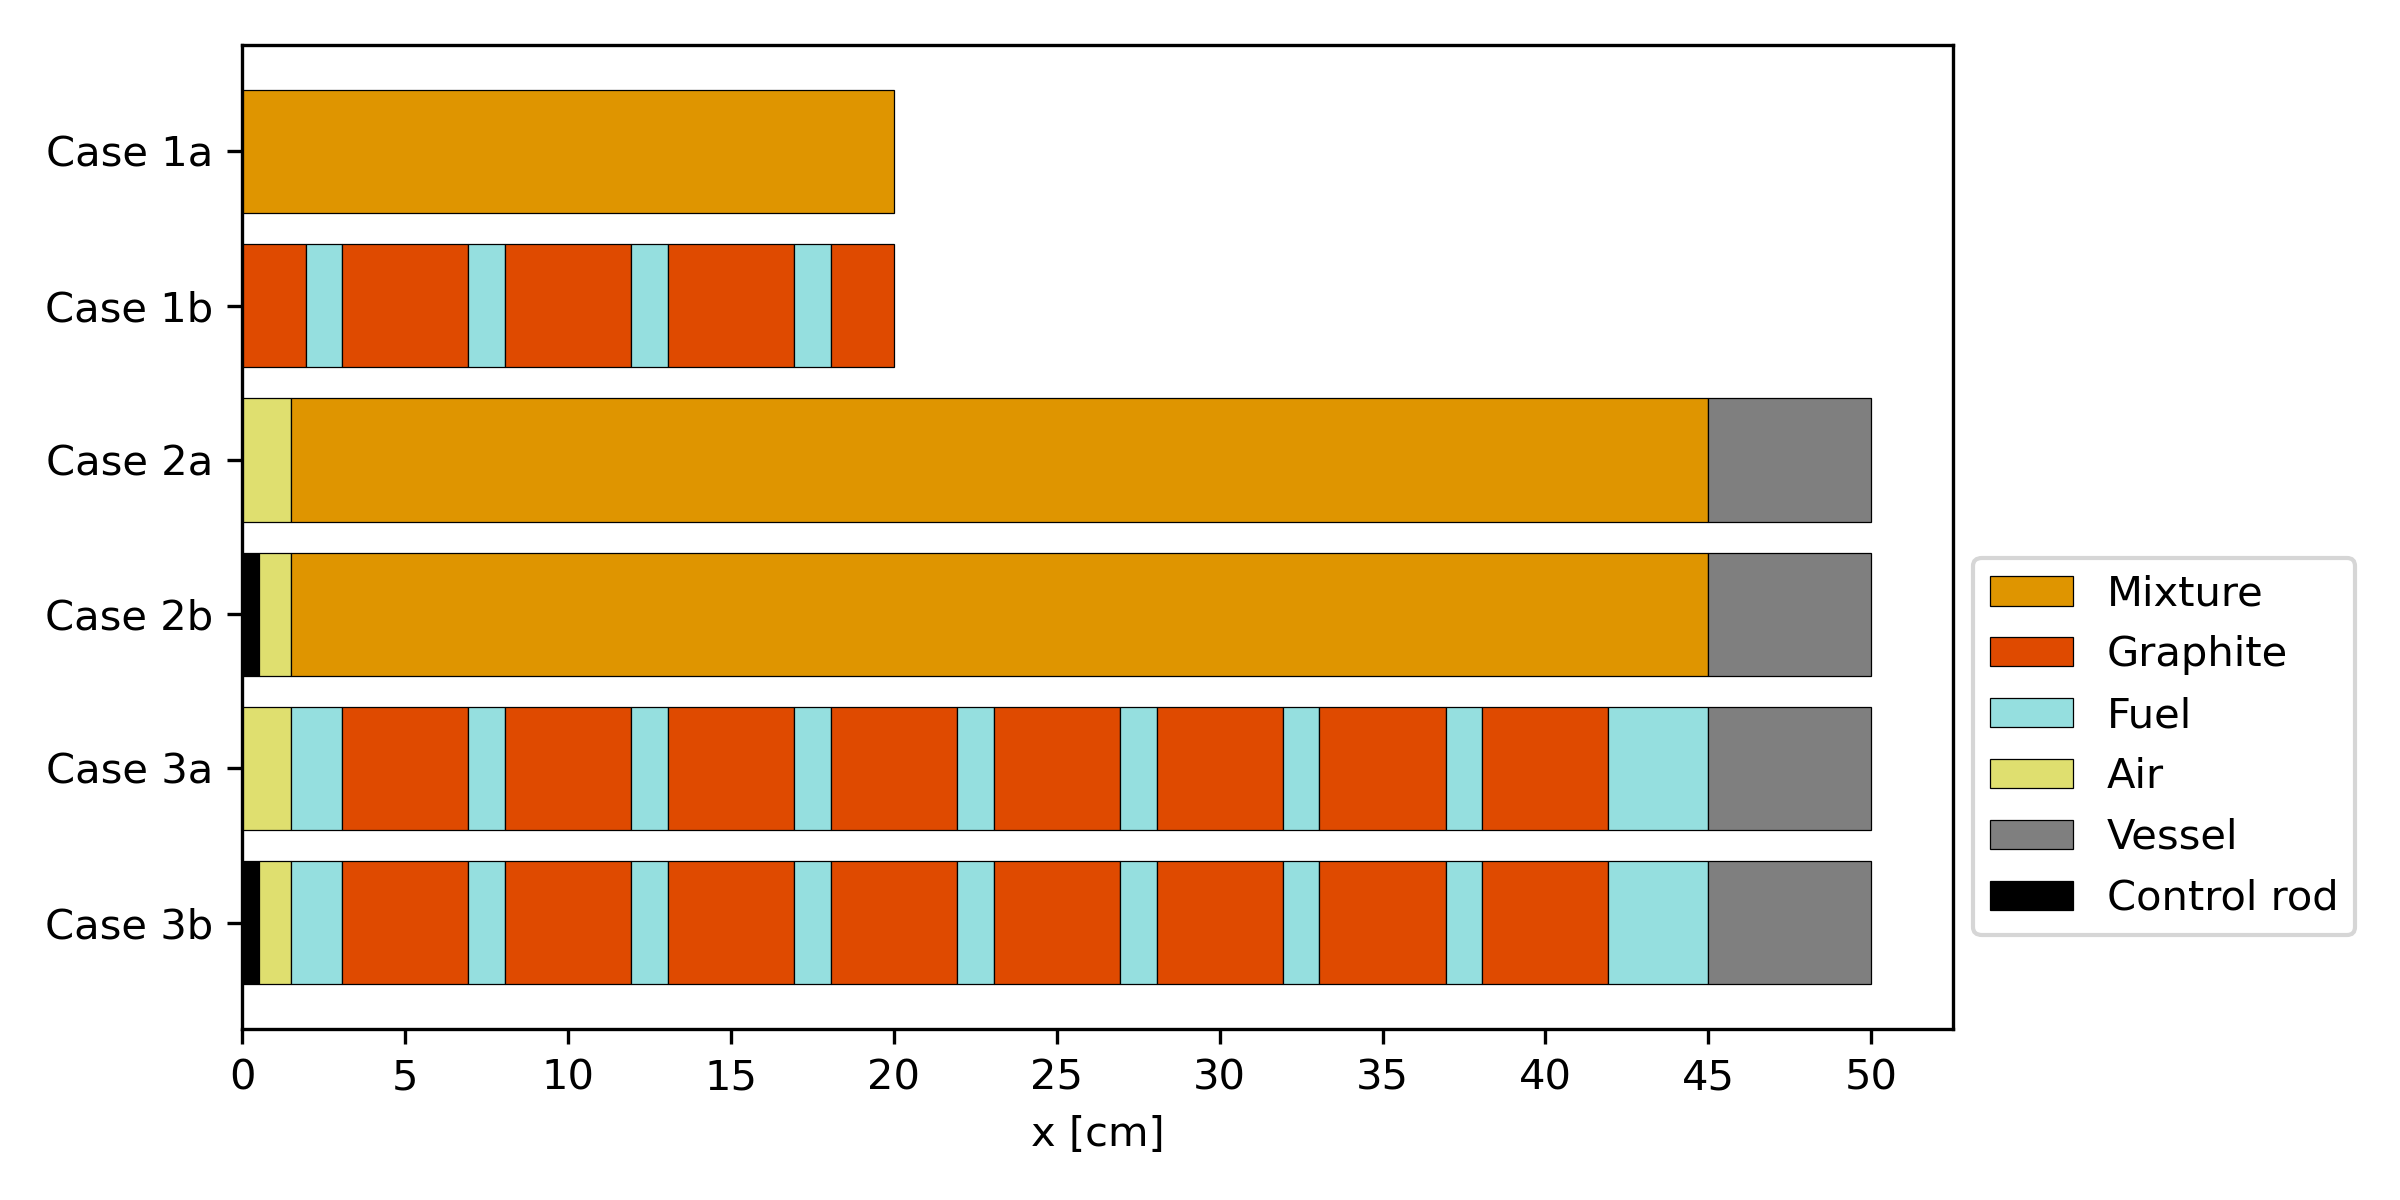
\includegraphics[width=0.8\columnwidth]{case-geometry}
  \caption{Geometries of the 1-D test cases. The material labeled ``mixture'' represents a
    homogeneous mixture of fuel and graphite at a ratio of 22.5\%-77.5\% by volume. All geometries
    have reflective boundary conditions on the boundary at $x=0$ cm. The right-side boundaries are
    reflective for Cases 1a and 1b, and vacuum for Cases 2a, 2b, 3a, and 3b.}
  \label{fig:case-geom}
\end{figure}

Cases 1a and 1b are simple test cases containing neutron multiplying regions. Cases 1a and 1b serve
to verify basic neutronics phenomena modeling (e.g., fission, scattering, absorption) of the newly
implemented $S_N$ and neutron diffusion methods in Python and $S_N$ method in Moltres. I did not
apply the hybrid method on these cases. Cases 2a and 2b represent 1-D models of the \gls{MSRE} with
air-filled control rod guide tube regions, a homogenized fuel-graphite lattice regions, and outer
vessel regions. Case 2b additionally contains a 0.5cm-thick control rod region to contrast with
Case 2a for control rod worth calculations. Cases 3a and 3b retain the heterogeneous fuel-graphite
lattice geometry present in the \gls{MSRE}.

In my preliminary investigations, the original control rod material composition
(70 wt\% Gd$_2$O$_3$-30 wt\% Al$_2$O$_3$) led to excessively large control rod worth estimates of
approximately 55000 pcm in the 1-D models, effectively halving the $k_\text{eff}$. The worth
estimates are ten times larger
than the 5500 pcm expected from full rod insertion of all three rods in the actual \gls{MSRE}
\cite{fratoni_molten_2020}. Therefore, I greatly reduced the proportion of Gd$_2$O$_3$ in the
control rod to 0.35 wt\% for a fairer assessment of rod worth in the 1-D models. This change
brought the new rod worth estimates down to below 20000 pcm.

\subsection{1-D Neutronics Model Mesh Convergence Tests}

I ran mesh convergence studies based on Case 3b for the neutron diffusion and $S_N$ neutron
transport methods. Given that the hybrid $S_N$-diffusion method comprises of a combination of those
methods, I found hybrid simulations were fully spatially resolved on meshes that are
appropriately resolved for both neutron diffusion and $S_N$ simulations.

\begin{figure}[htb!]
  \centering
  \begin{subfigure}[b]{0.48\columnwidth}
    \centering
    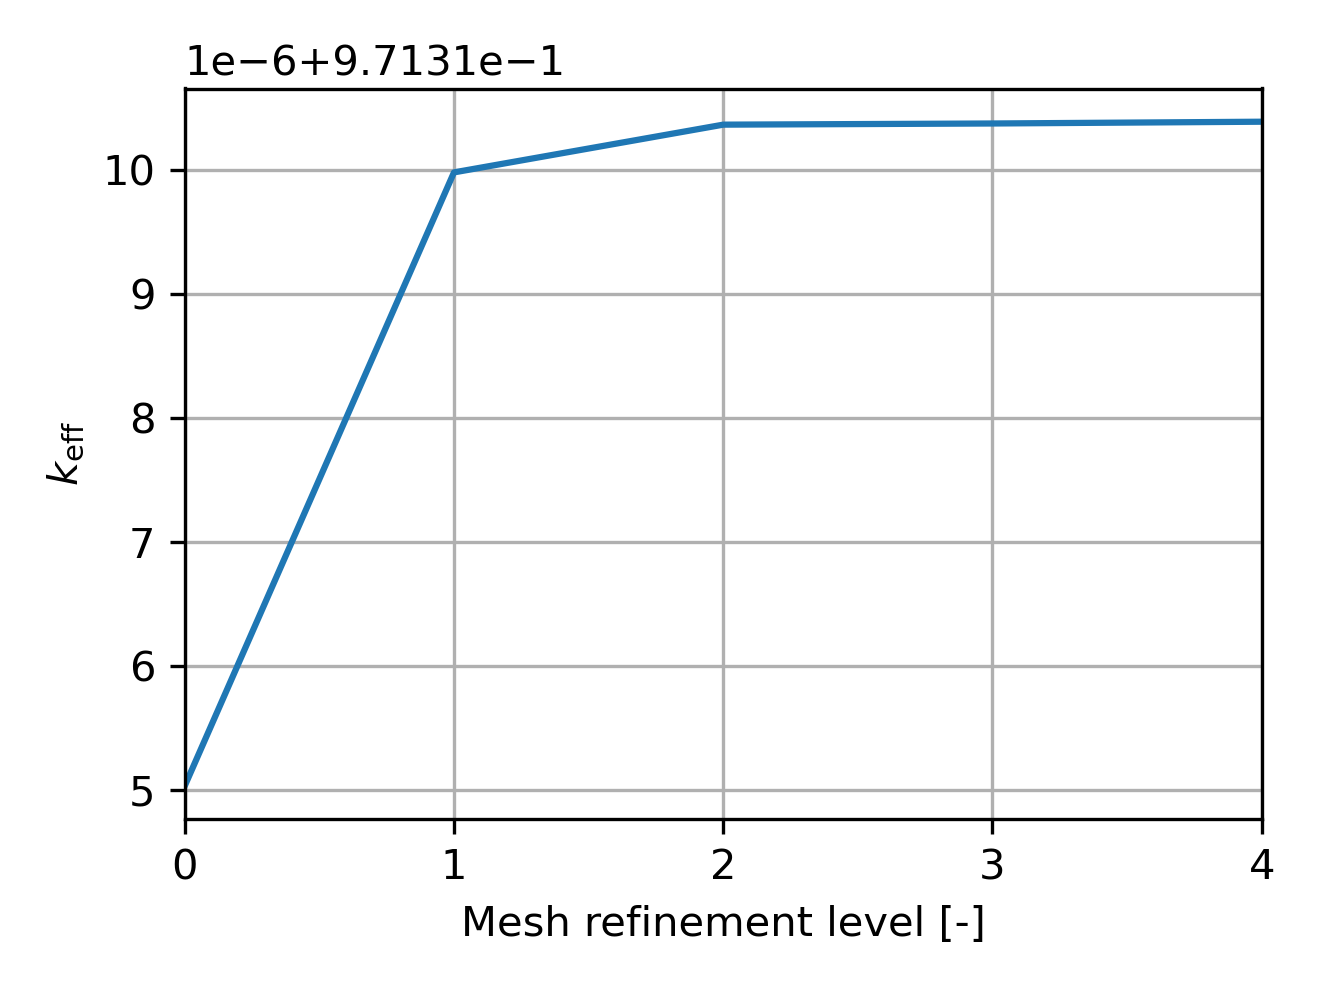
\includegraphics[width=\columnwidth]{diffusion-mesh-convergence-k}
    \caption{Neutron diffusion method}
    \label{fig:diff-mesh-k}
  \end{subfigure}
  \hfill
  \begin{subfigure}[b]{0.48\columnwidth}
    \centering
    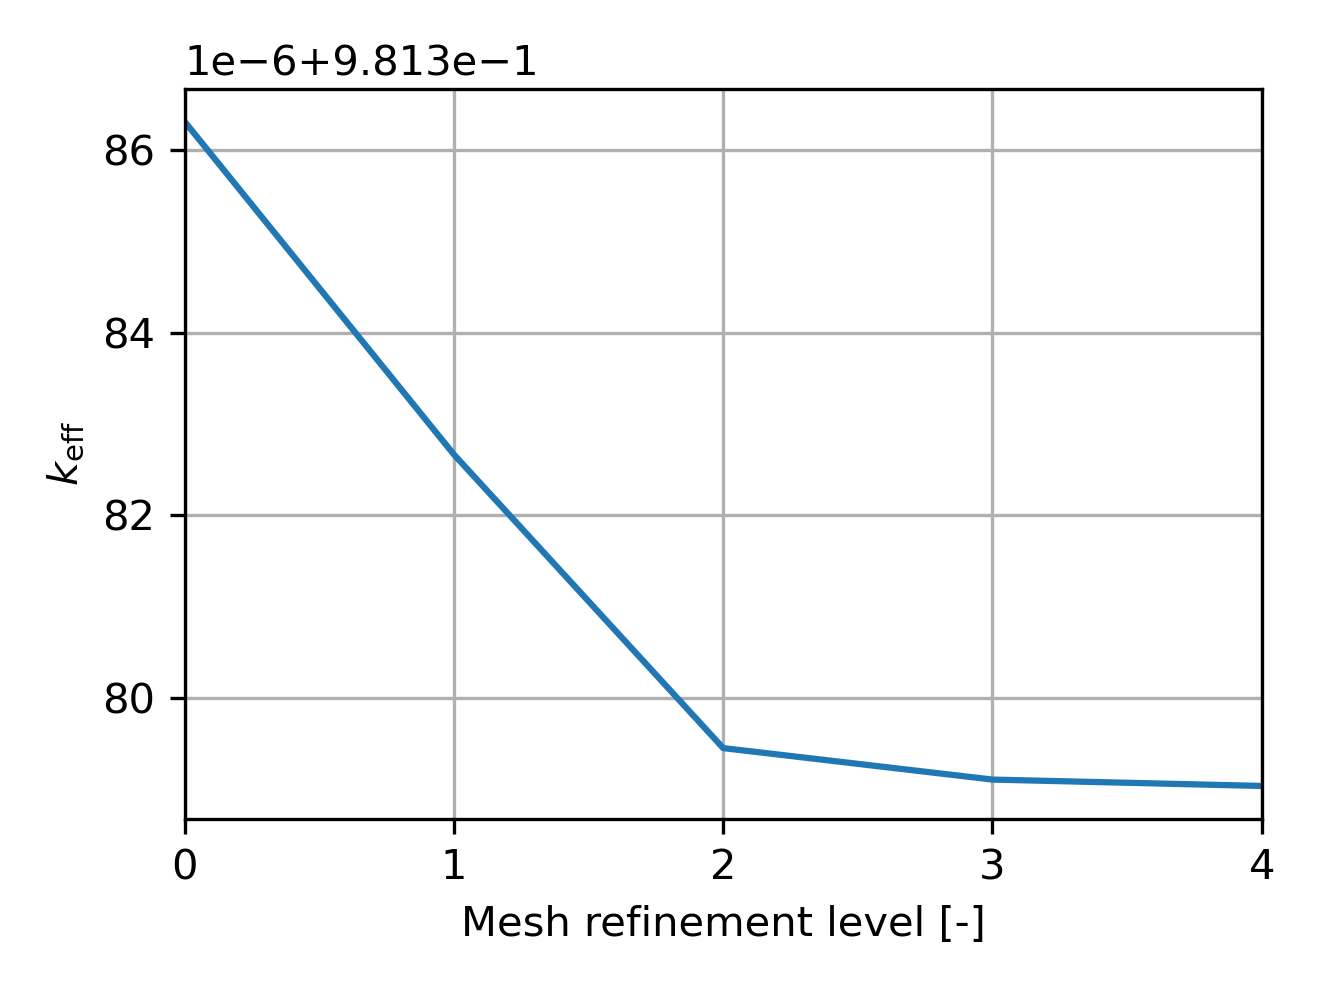
\includegraphics[width=\columnwidth]{sn-mesh-convergence-k}
    \caption{$S_8$ neutron transport method}
    \label{fig:sn-mesh-k}
  \end{subfigure}
  \caption{Convergence of multiplication factor ($k_\text{eff}$) estimates for Case 3b across five
    levels of mesh refinement. Higher refinement levels correspond to smaller mesh element sizes.}
  \label{fig:mesh-k}
\end{figure}

Figures \ref{fig:diff-mesh-k} and \ref{fig:sn-mesh-k} show the convergence of $k_\text{eff}$
estimates observed for Case 3b simulations with neutron diffusion and $S_8$ neutron transport
methods. The $k_\text{eff}$ values plateau at 0.9713203 and 0.9813790 for the neutron diffusion and
$S_8$ methods, respectively. By mesh refinement level 2, both methods fall within $5\times 10^{-7}$
range of the $k_\text{eff}$ value at level 4.

Figures \ref{fig:diff-mesh-flux} and \ref{fig:sn-mesh-flux} show the absolute differences in the
group flux distributions at mesh refinement levels 1 to 3 relative to the reference group flux
distribution at level 4 (maximum refinement). I omitted data from level 0 to improve the fidelity
of the plots as flux differences drop significantly by one order of magnitude with each level of
refinement.
With these results, I concluded that the mesh resolution at level 2 is a sufficient guideline for
the mesh resolutions used in the subsequent 1-D analyses. The absolute differences in both
$k_\text{eff}$ and group flux distributions at level 2 remain below $5\times10^{-7}$ relative to
level 4.

\begin{figure}[htb!]
  \centering
  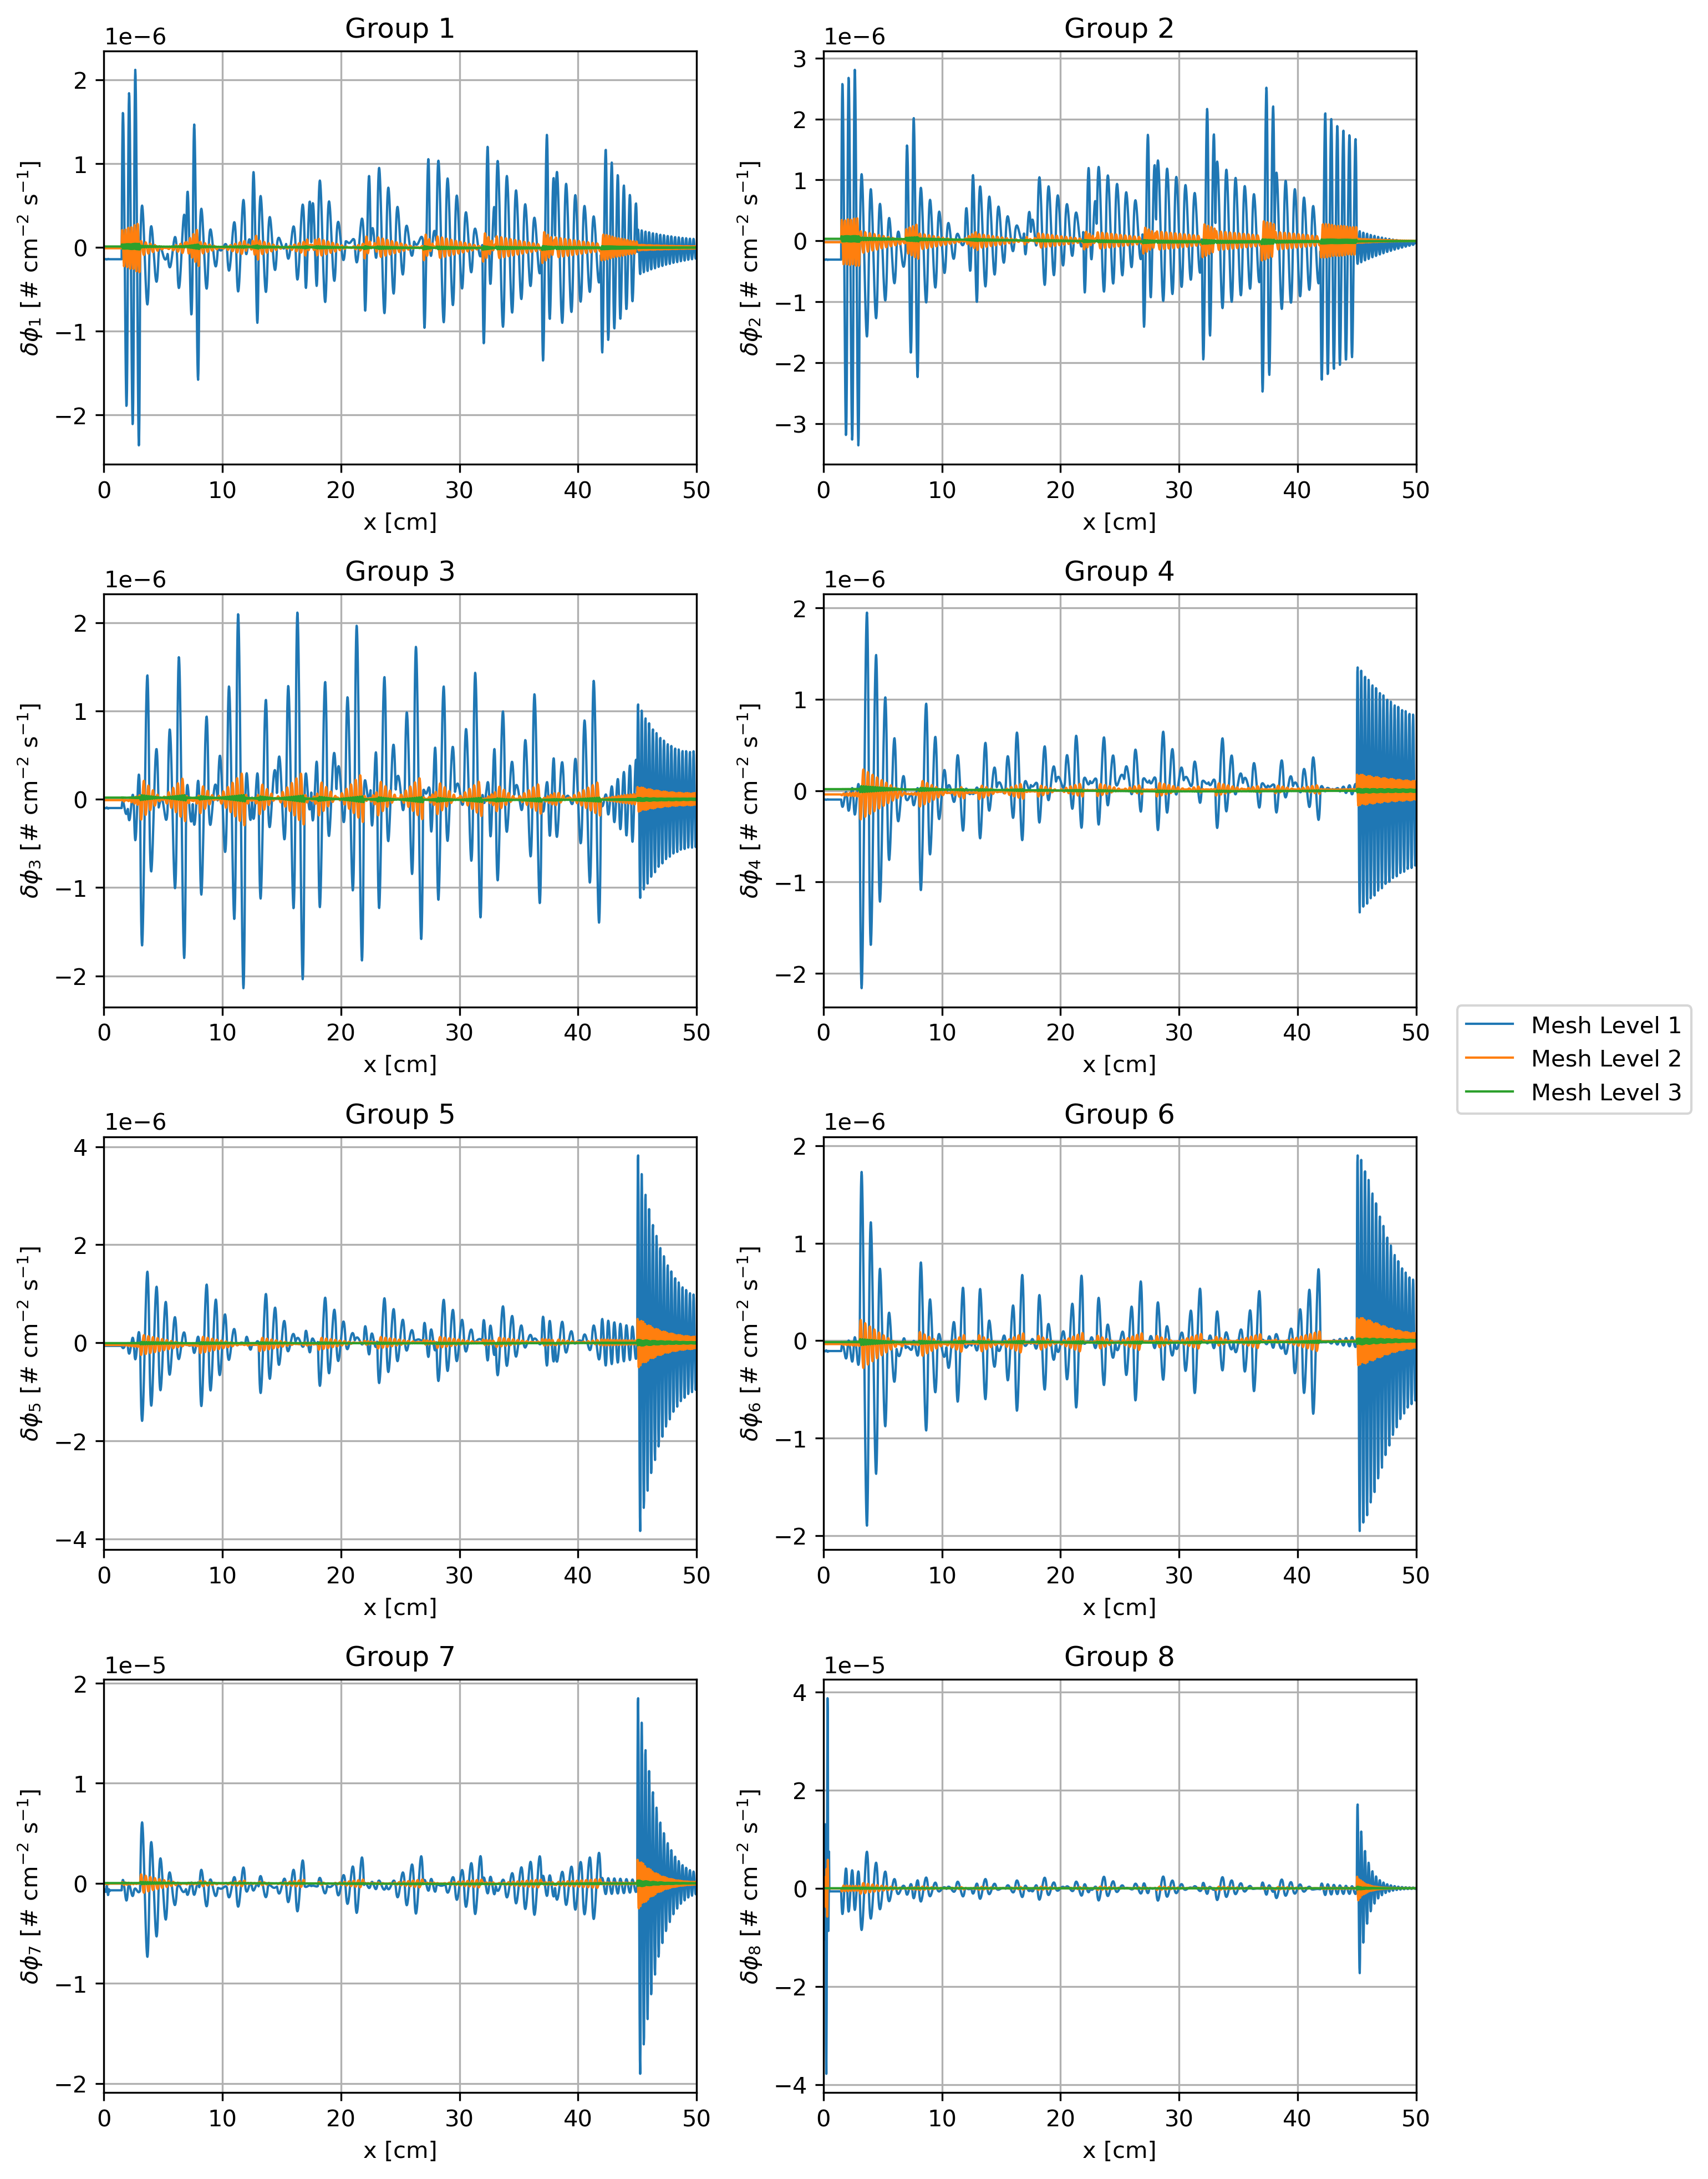
\includegraphics[width=\columnwidth]{diffusion-mesh-convergence-flux}
  \caption{Absolute difference in group fluxes ($\phi_g$) from the neutron diffusion method for
  mesh refinement levels 1 to 4 relative to the reference group flux distributions at mesh
  refinement level 5.}
  \label{fig:diff-mesh-flux}
\end{figure}

\begin{figure}[htb!]
  \centering
  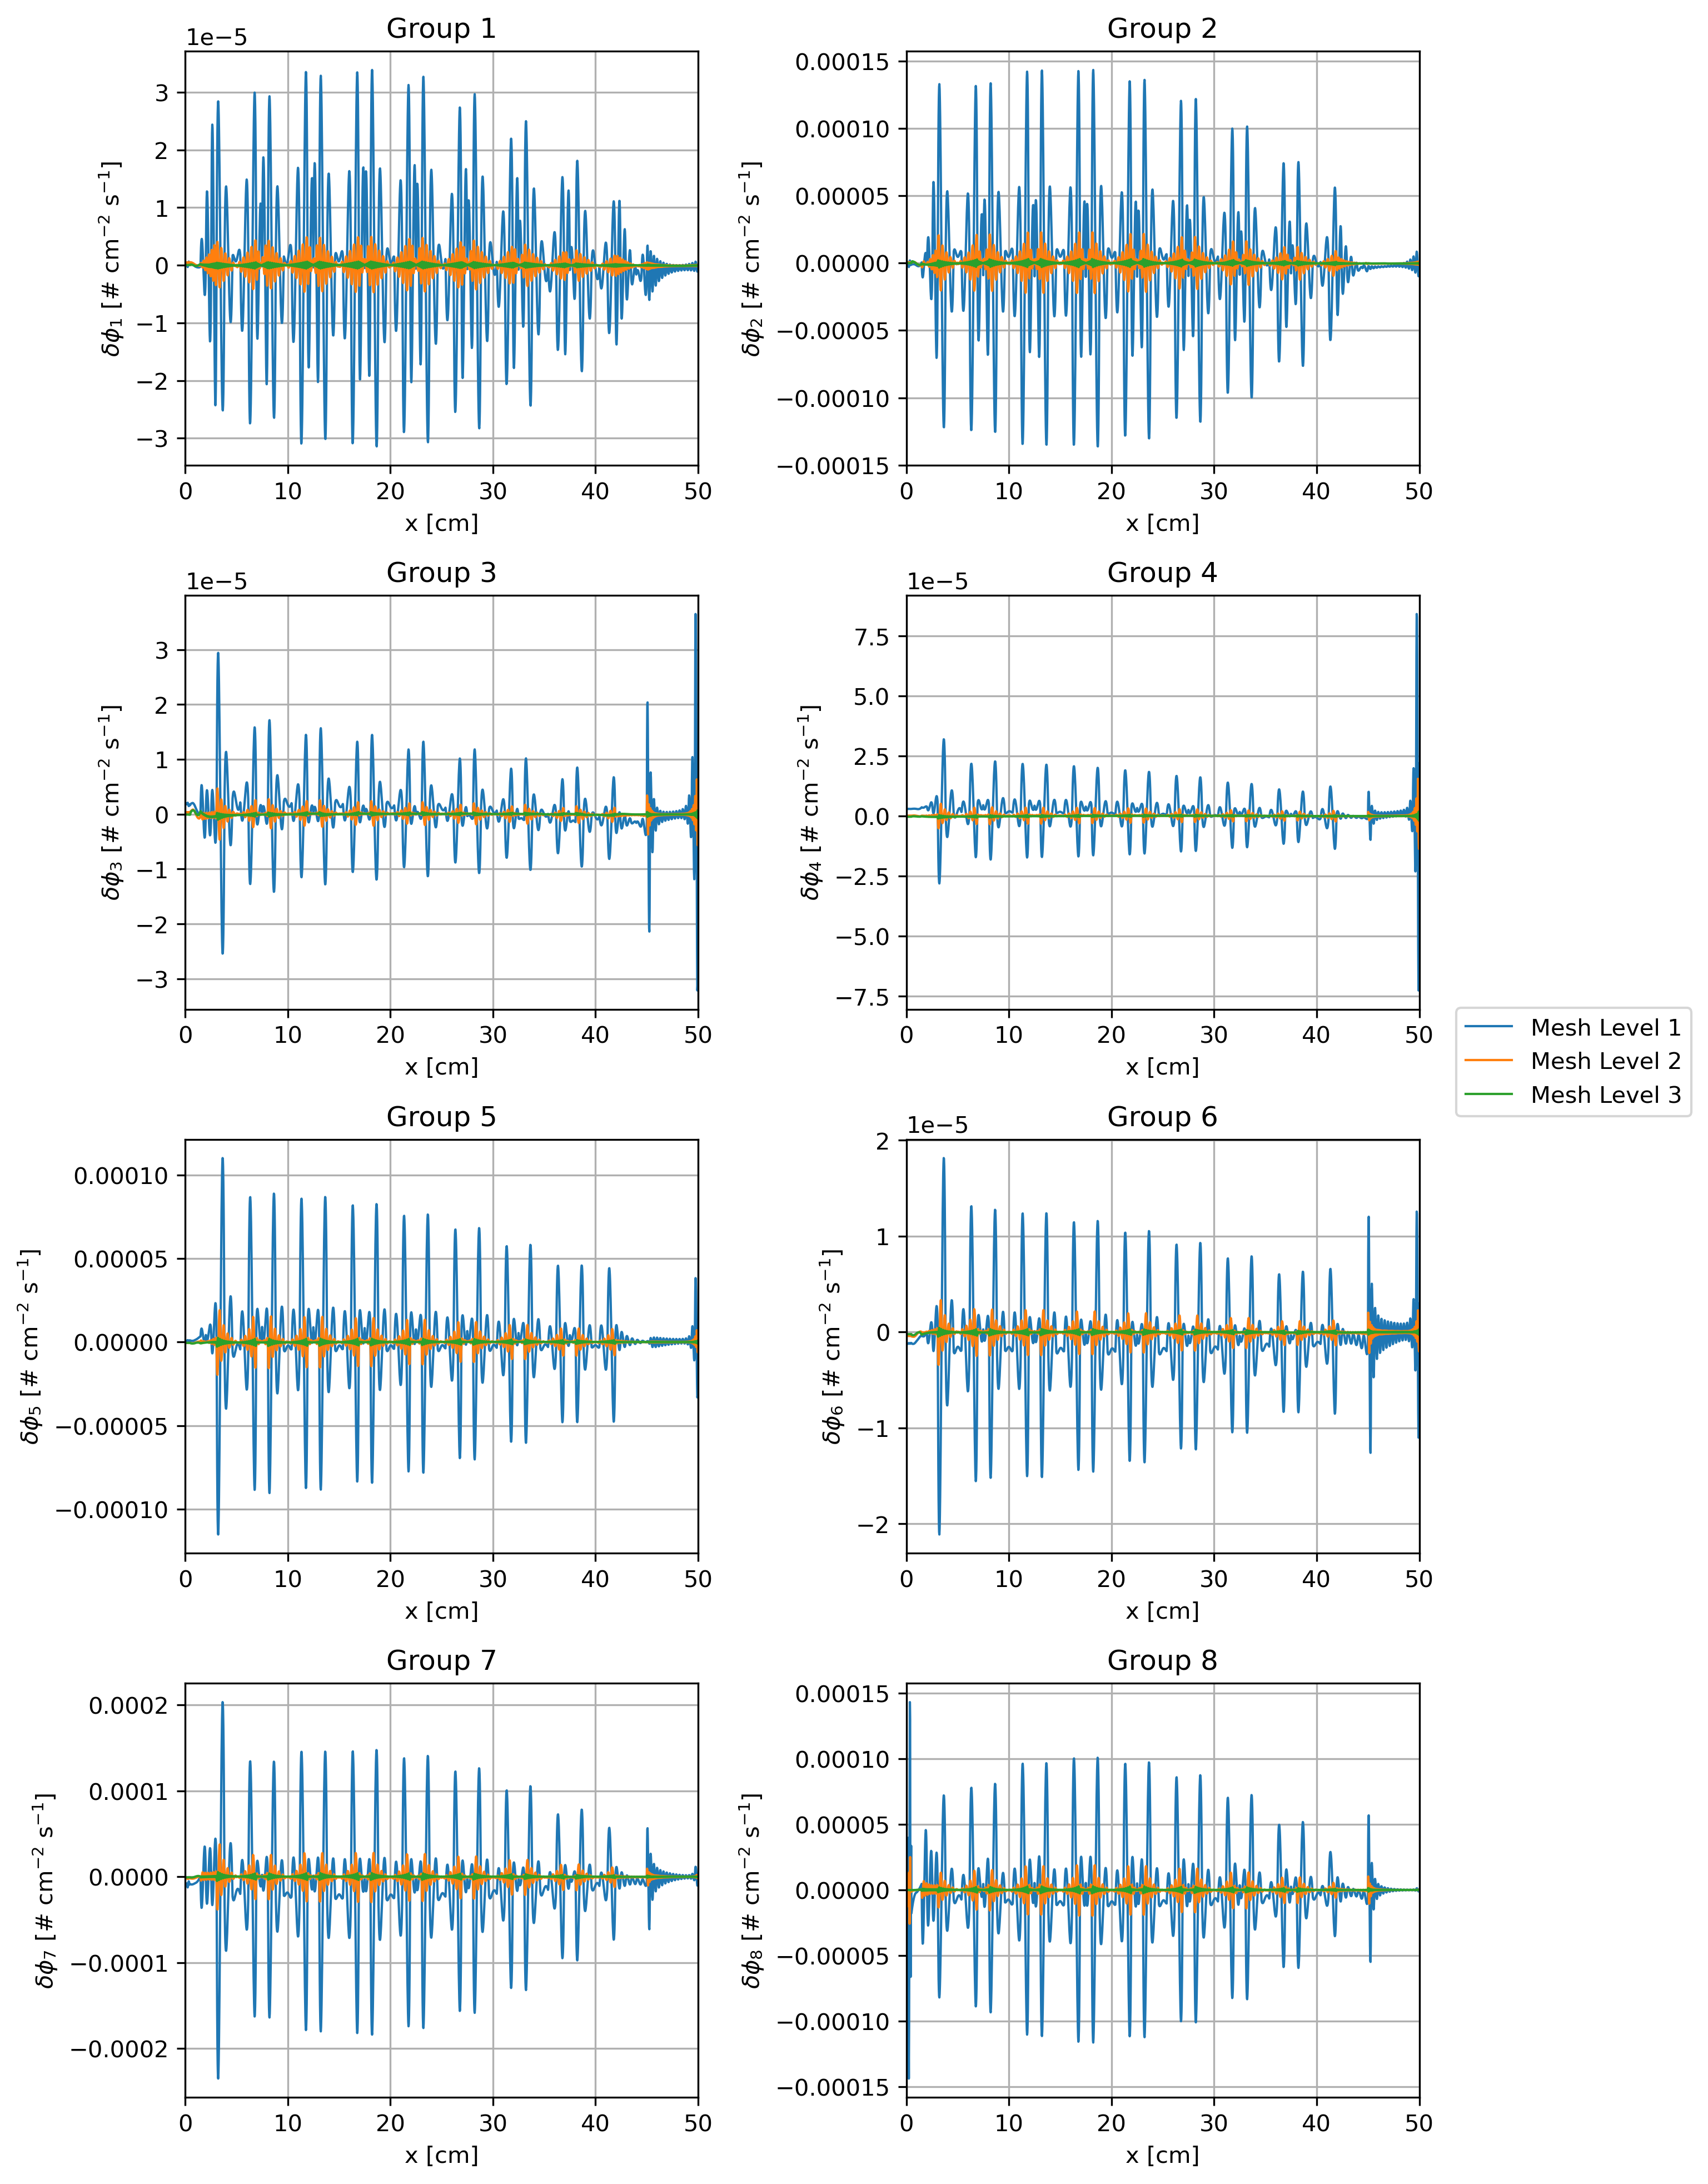
\includegraphics[width=\columnwidth]{sn-mesh-convergence-flux}
  \caption{Absolute difference in group fluxes ($\phi_g$) from the $S_8$ neutron transport method
  for mesh refinement levels 1 to 4 relative to the reference group flux distributions at mesh
  refinement level 5.}
  \label{fig:sn-mesh-flux}
\end{figure}

\FloatBarrier

\subsection{1-D Neutronics Numerical Results \& Discussion}

\subsubsection{Reactivity}

Figure \ref{fig:1d-rho} shows the difference in reactivities of OpenMC-MG, $S_8$,
neutron diffusion, and hybrid methods relative to OpenMC-CE. The standard deviations of
reactivity values from OpenMC-CE are approximately 40 pcm for Cases 1a and 1b and 60 pcm for the
rest as depicted by the blue highlighted area in Figure \ref{fig:1d-rho}. For Cases 1a and 1b, the
OpenMC-MG, $S_8$, and neutron diffusion methods show excellent agreement with OpenMC-CE as the
reactivity values fall within the one or two standard deviation range. The Case 1 results show
the Moltres and Python implementations are consistent with each other given that they are spatially
well-resolved.

\begin{figure}[htb!]
  \centering
  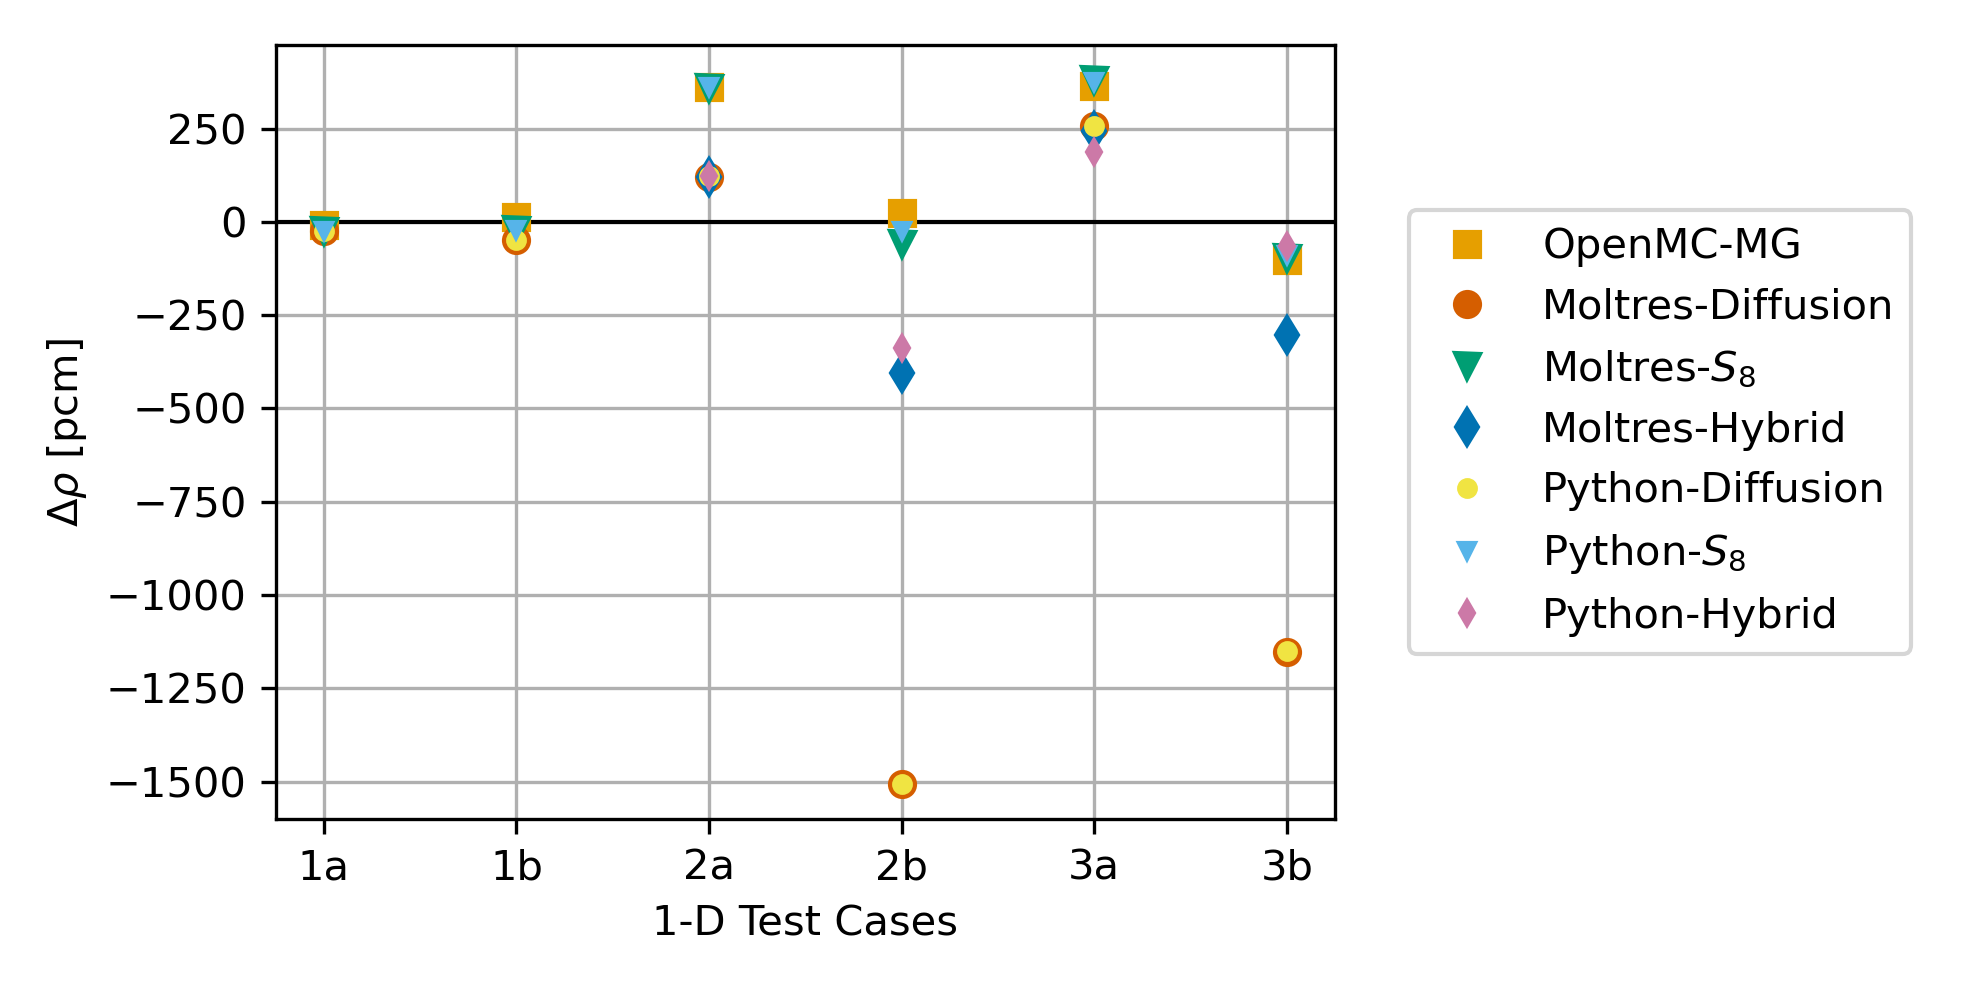
\includegraphics[width=\columnwidth]{rho}
  \caption{Difference in reactivity $\rho$ of all neutronics methods investigated relative
  to OpenMC-CE.}
  \label{fig:1d-rho}
\end{figure}

For all cases, the OpenMC-MG and the $S_8$ methods show consistent agreement with one another. 
While they deviate from OpenMC-CE by approximately 350 pcm for Cases 2a and 3a, they fall within
two standard deviations of OpenMC-CE for Cases 2b and 3b. When increasing the maximum Legendre
polynomial order to approximate the angular dependence in $\Sigma_s^{g'\rightarrow g}$ from
2nd-order to 3rd-order, the reactivity changed by only 1 pcm. Therefore, I attribute the reactivity
discrepancies to the eight neutron energy group structure which remains the
only significant difference between OpenMC-CE and the multigroup methods.

The neutron diffusion and hybrid methods agree closely with one another for Cases 2a and 3a which
exclude the control rod region. This shows that the hybrid method provides similar $k_\text{eff}$
estimates to the neutron diffusion method in 1-D simulations without highly neutron-absorbing
regions. Compared to the OpenMC-MG and $S_8$ reactivity values, the neutron diffusion and hybrid
method reactivity values agree closer with the reference OpenMC-CE value. However, this is likely
due to favorable error cancellation; Figures \ref{fig:3a-flux} and \ref{fig:3a-flux-diff} show
OpenMC-MG and the $S_8$ methods reproduce
the OpenMC-CE flux distribution more accurately than the neutron diffusion and hybrid methods.

In Cases 2b and 3b, the neutron diffusion method largely fails to accurately capture the
effect of introducing the control rod region as evidenced by the -1500 pcm and -1150 pcm
discrepancies relative to OpenMC-CE. The hybrid method fares better with -400 pcm and -300 pcm
discrepancies.

\begin{figure}[htb!]
  \centering
  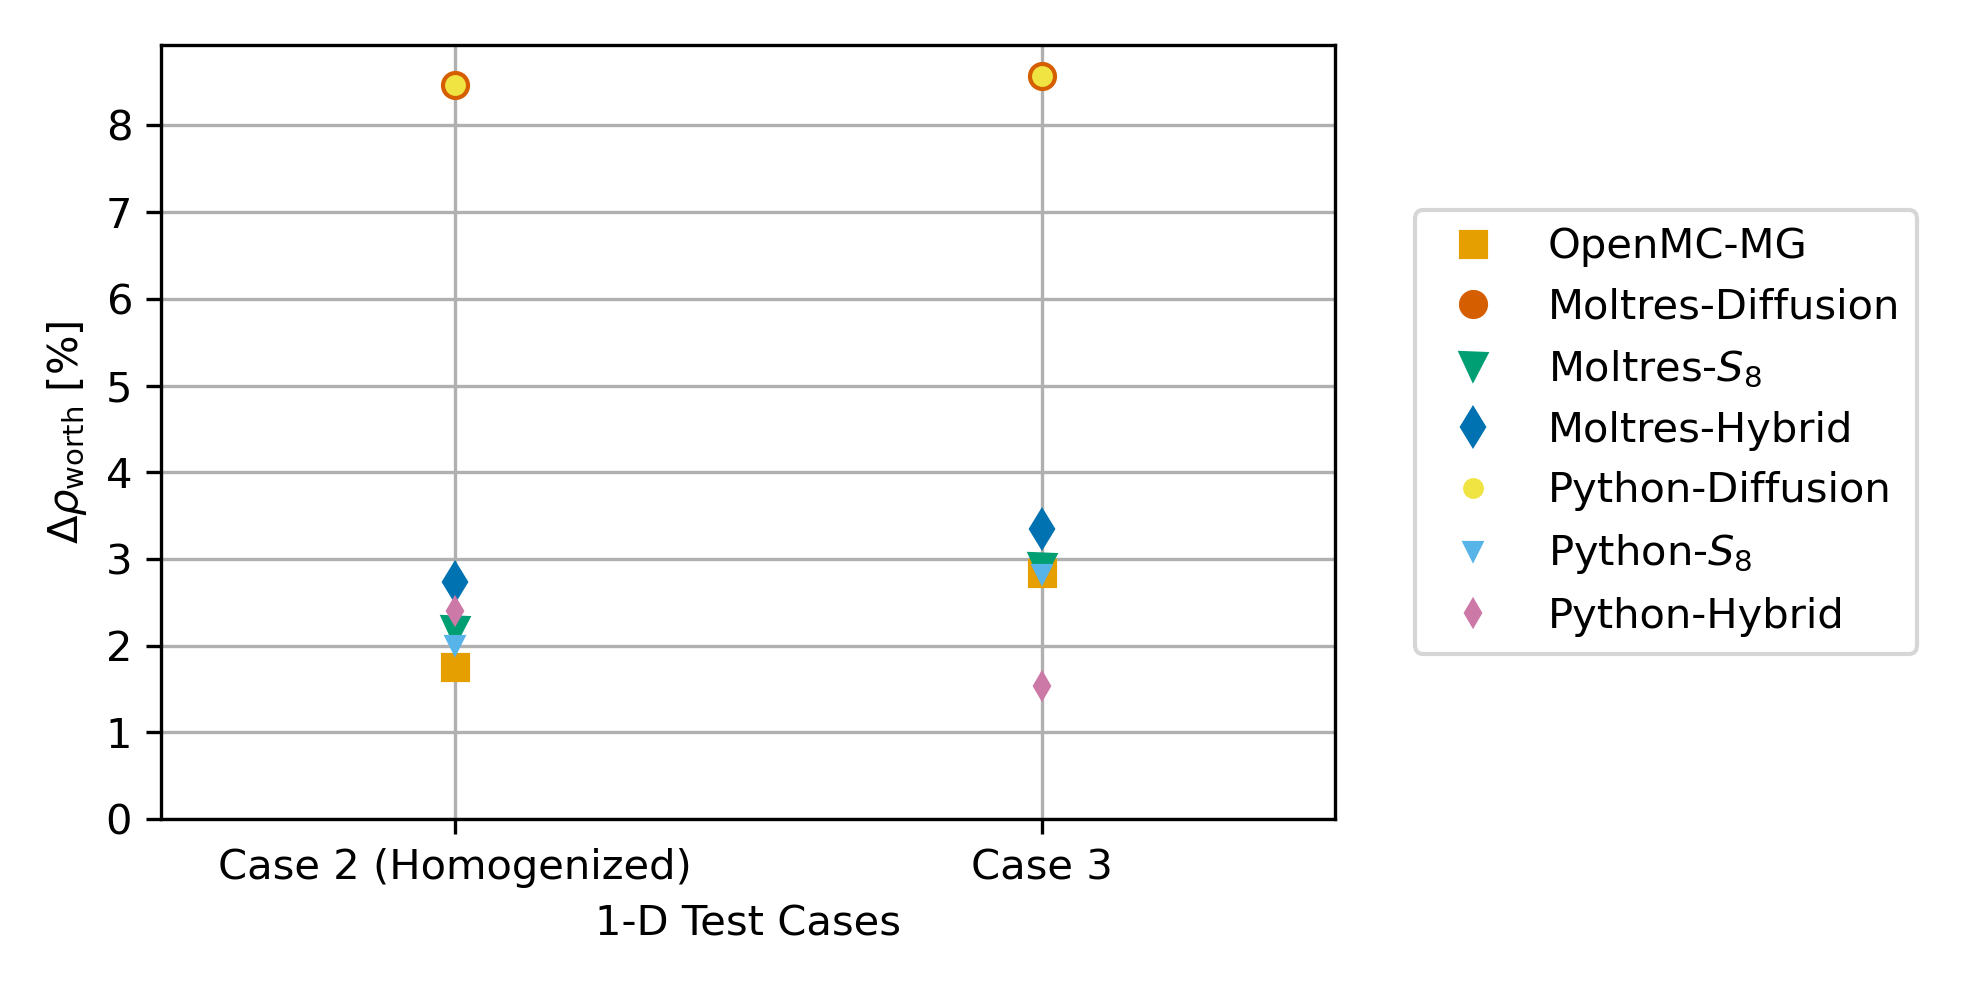
\includegraphics[width=\columnwidth]{worth}
  \caption{Percentage difference in rod worth for Cases 2 and 3 of all neutronics methods
  investigated relative to OpenMC-CE.}
  \label{fig:1d-worth}
\end{figure}

\subsubsection{Control rod worth}

Moving the discussion to control rod worths, figure \ref{fig:1d-worth} shows the percentage
difference in rod worths for Cases 2 and 3 of OpenMC-MG, $S_8$, neutron diffusion, and hybrid
methods relative to OpenMC-CE. I calculated the rod worth estimates from each method by taking the
difference in reactivity between the ``rod out'' (a) and ``rod in'' (b) configurations of Cases 2
and 3. All neutronics methods overestimate the rod worth relative to OpenMC-CE, resulting in
positive percentage difference values observed in the figure.
The neutron diffusion methods clearly show up as outliers with rod worth estimates in excess
of 8\%. Most of the remaining methods cluster around 2.5\% and 3\% percentage difference for Cases
2 and 3 with the exception of the Python-hybrid method for Case 3.

Given that the hybrid methods rely on transport corrections derived from the $S_N$ method, the
$S_8$ rod worth estimates serve as the
reference point for hybrid method verification. Additionally, errors arising from the multigroup
approximation affect both hybrid and $S_N$ simulations to similar degrees. While the Python-hybrid
method produces the lowest percentage difference relative to OpenMC-CE for Case 3, the
Python-hybrid method deviates from the $S_8$ ``multigroup'' reference rod worths more than the
Moltres-hybrid method. Nevertheless, both hybrid method implementations provide significant
improvements in rod worth estimates over the neutron diffusion method.

\subsubsection{Neutron flux distribution}

This discussion on the neutron flux distributions focuses on Cases 3a and 3b which most closely
resemble the actual \gls{MSRE} reactor geometry. Cases 3a and 3b resemble the \gls{MSRE} reactor
with a control rod withdrawn and inserted, respectively. Figures \ref{fig:3a-flux} and
\ref{fig:3b-flux} show the neutron group flux distributions for Cases 3a and 3b from OpenMC-CE and
OpenMC-MG. Differences between the two methods arise from the multigroup approximation, notably in
group 2 for Case 3a and groups 2, 6, 7, 8 for Case 3b. Future work aimed at finding a better
neutron energy group structure should at minimum focus on improving fidelity in the listed energy
groups.

For a fair evaluation of the deterministic multigroup methods without distortions from the
multigroup approximation, I chose to compare their flux distributions with the OpenMC-MG flux
distribution. Figures \ref{fig:3a-flux-diff} and \ref{fig:3b-flux-diff} show the absolute
difference in neutron group flux distributions of the Moltres-$S_8$, Moltres-diffusion,
Moltres-hybrid, and Python-hybrid methods relative to OpenMC-MG. The figures omit Python-$S_8$ and
Python-diffusion as their distributions are nearly identical to their Moltres-based counterparts.
The neutron diffusion and hybrid methods fare worse than the $S_8$ method at capturing the
oscillatory pattern in groups 1, 2, 5, 7, and 8 arising from the fuel-graphite lattice geometry
along $x=5$ cm to 10 cm. In both Cases 3a and 3b, the neutron diffusion method (yellow plot lines)
exhibits significant flux deviations in groups 1, 2, 7, and 8 near $x=0$ cm.

Both hybrid methods
provide significant improvements in neutron flux distributions compared to the neutron diffusion
method as shown by the generally smaller flux difference values particularly near $x=0$ cm. The
figures also show Moltres-hybrid (green) provides more accurate flux estimates than
Python-hybrid (red) in all instances. The differences indicate deficiencies in the diffusion
correction scheme in Python-hybrid which lead to poorer performance compared to the drift
correction scheme in Moltres-hybrid.

\begin{figure}[htb!]
  \centering
  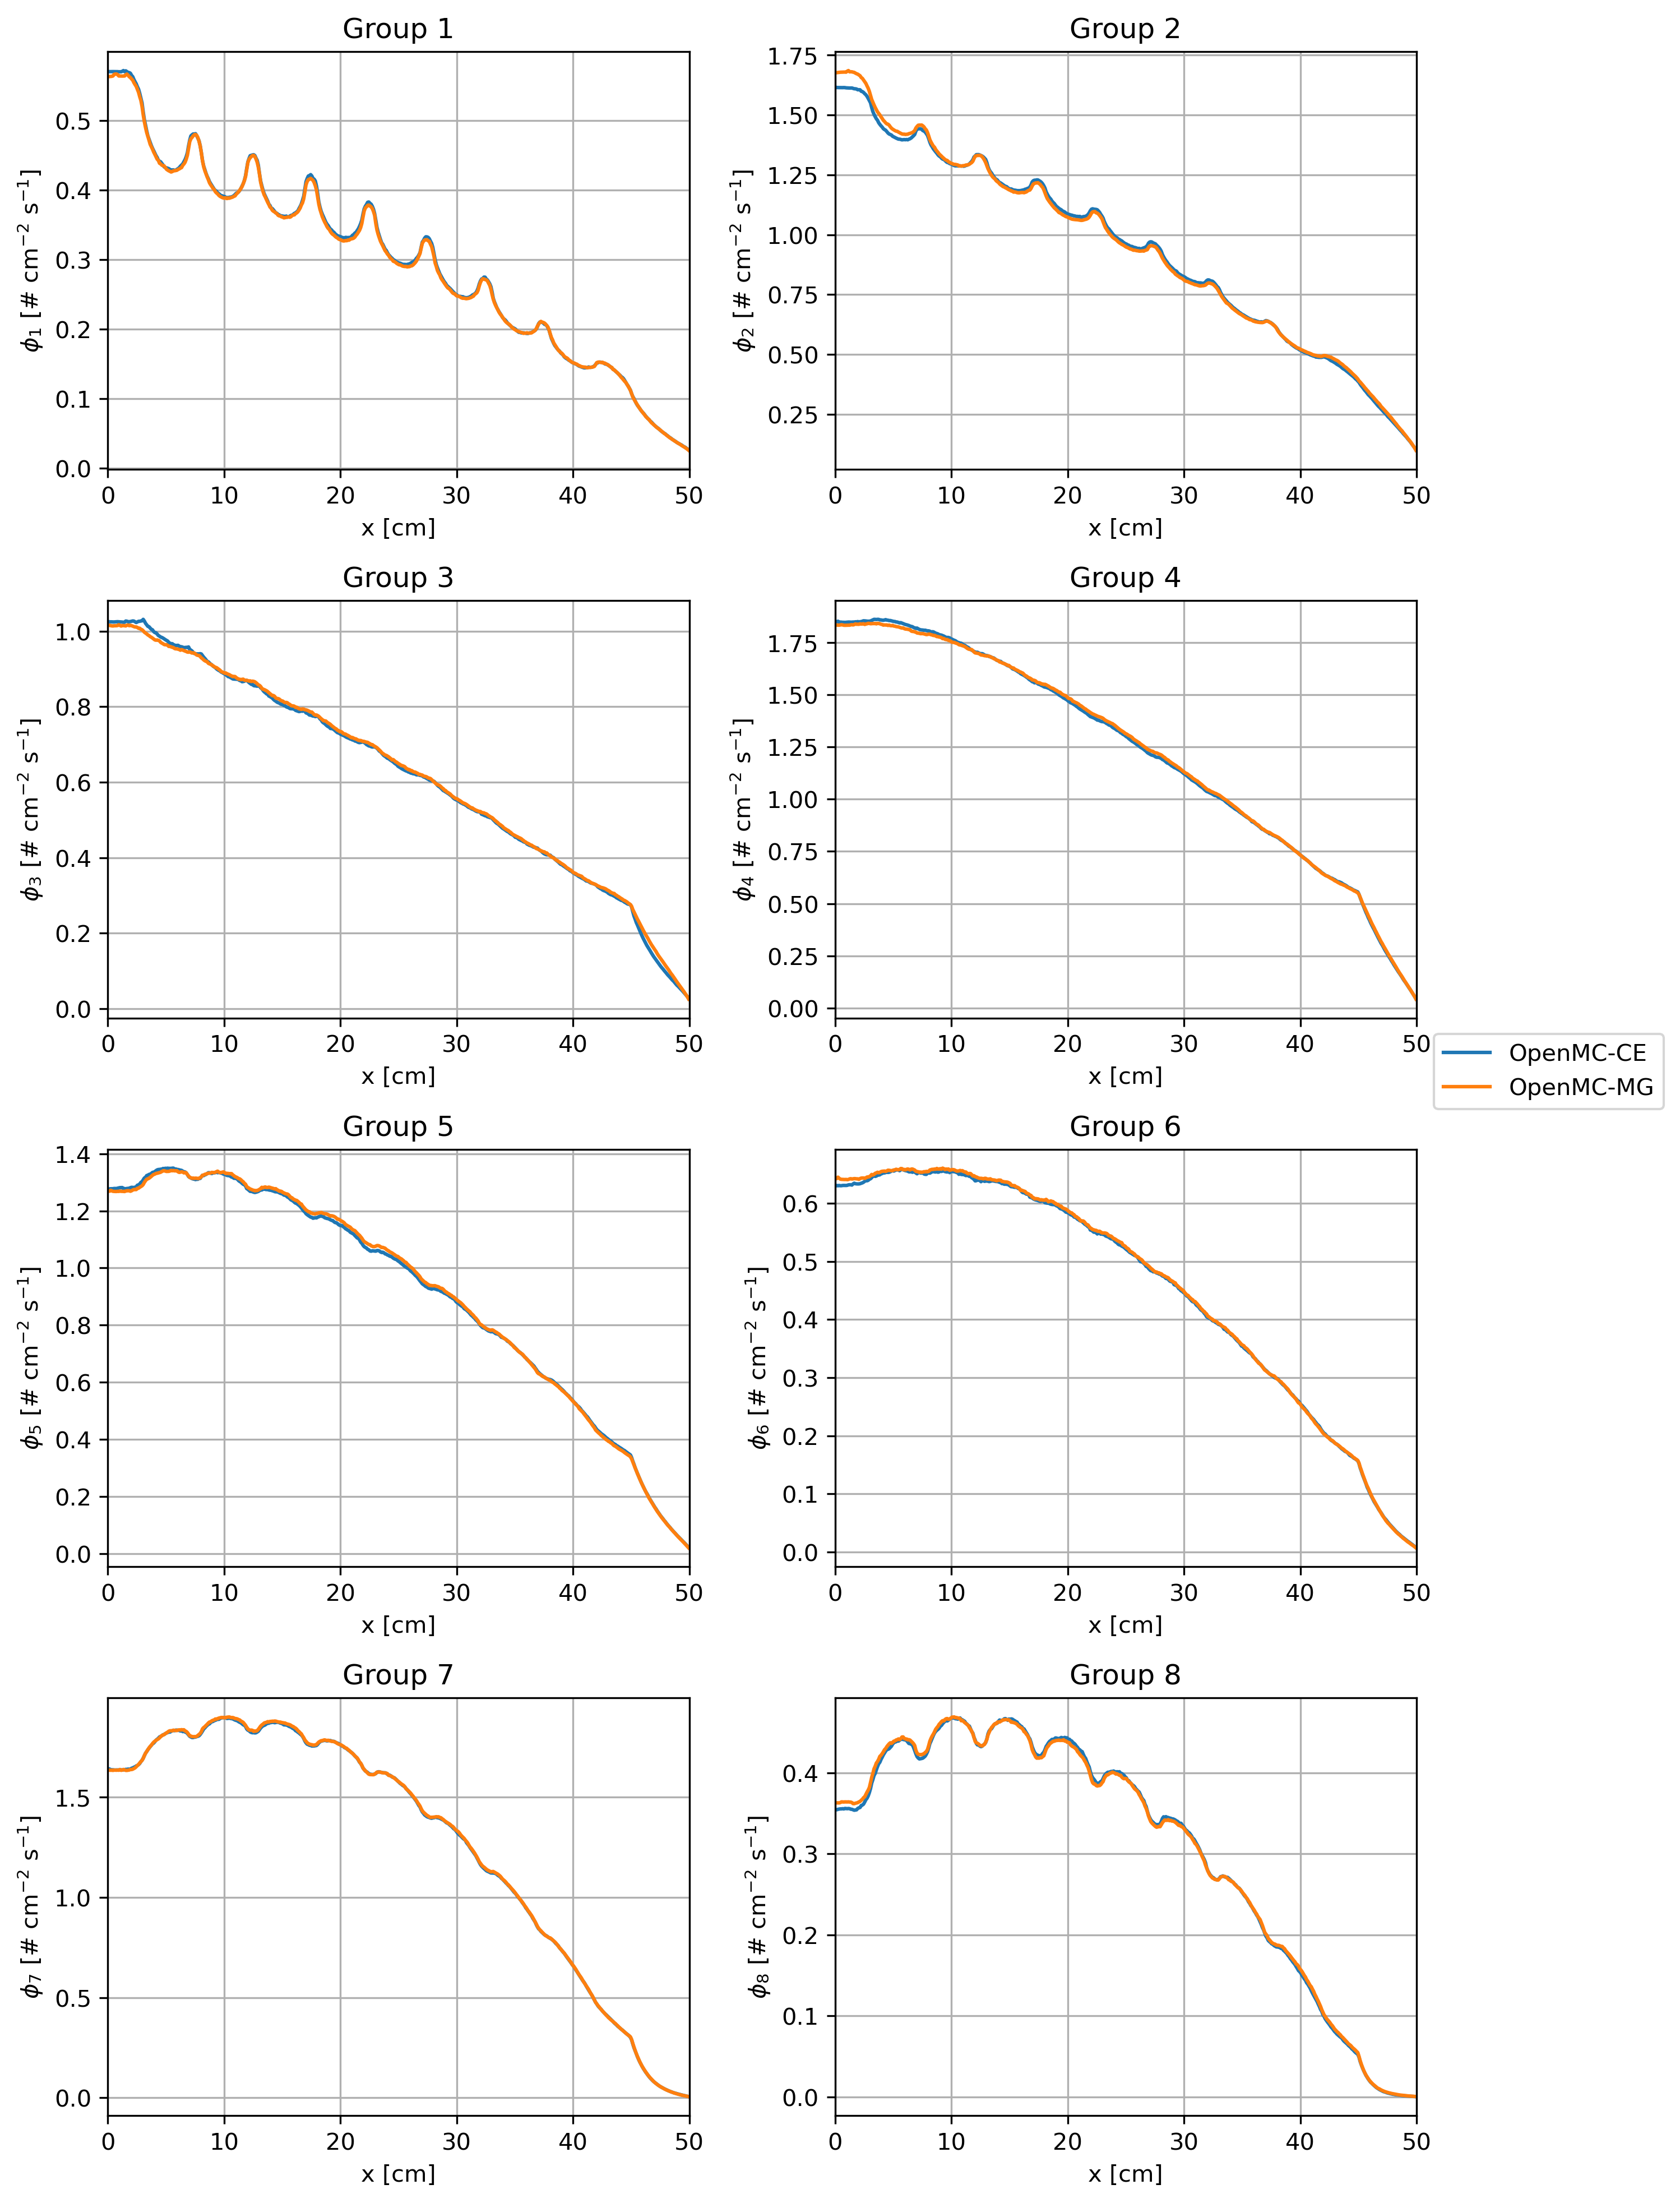
\includegraphics[width=\columnwidth]{case-3a-flux}
  \caption{Case 3a neutron group flux distributions from OpenMC-CE and OpenMC-MG.}
  \label{fig:3a-flux}
\end{figure}

\begin{figure}[htb!]
  \centering
  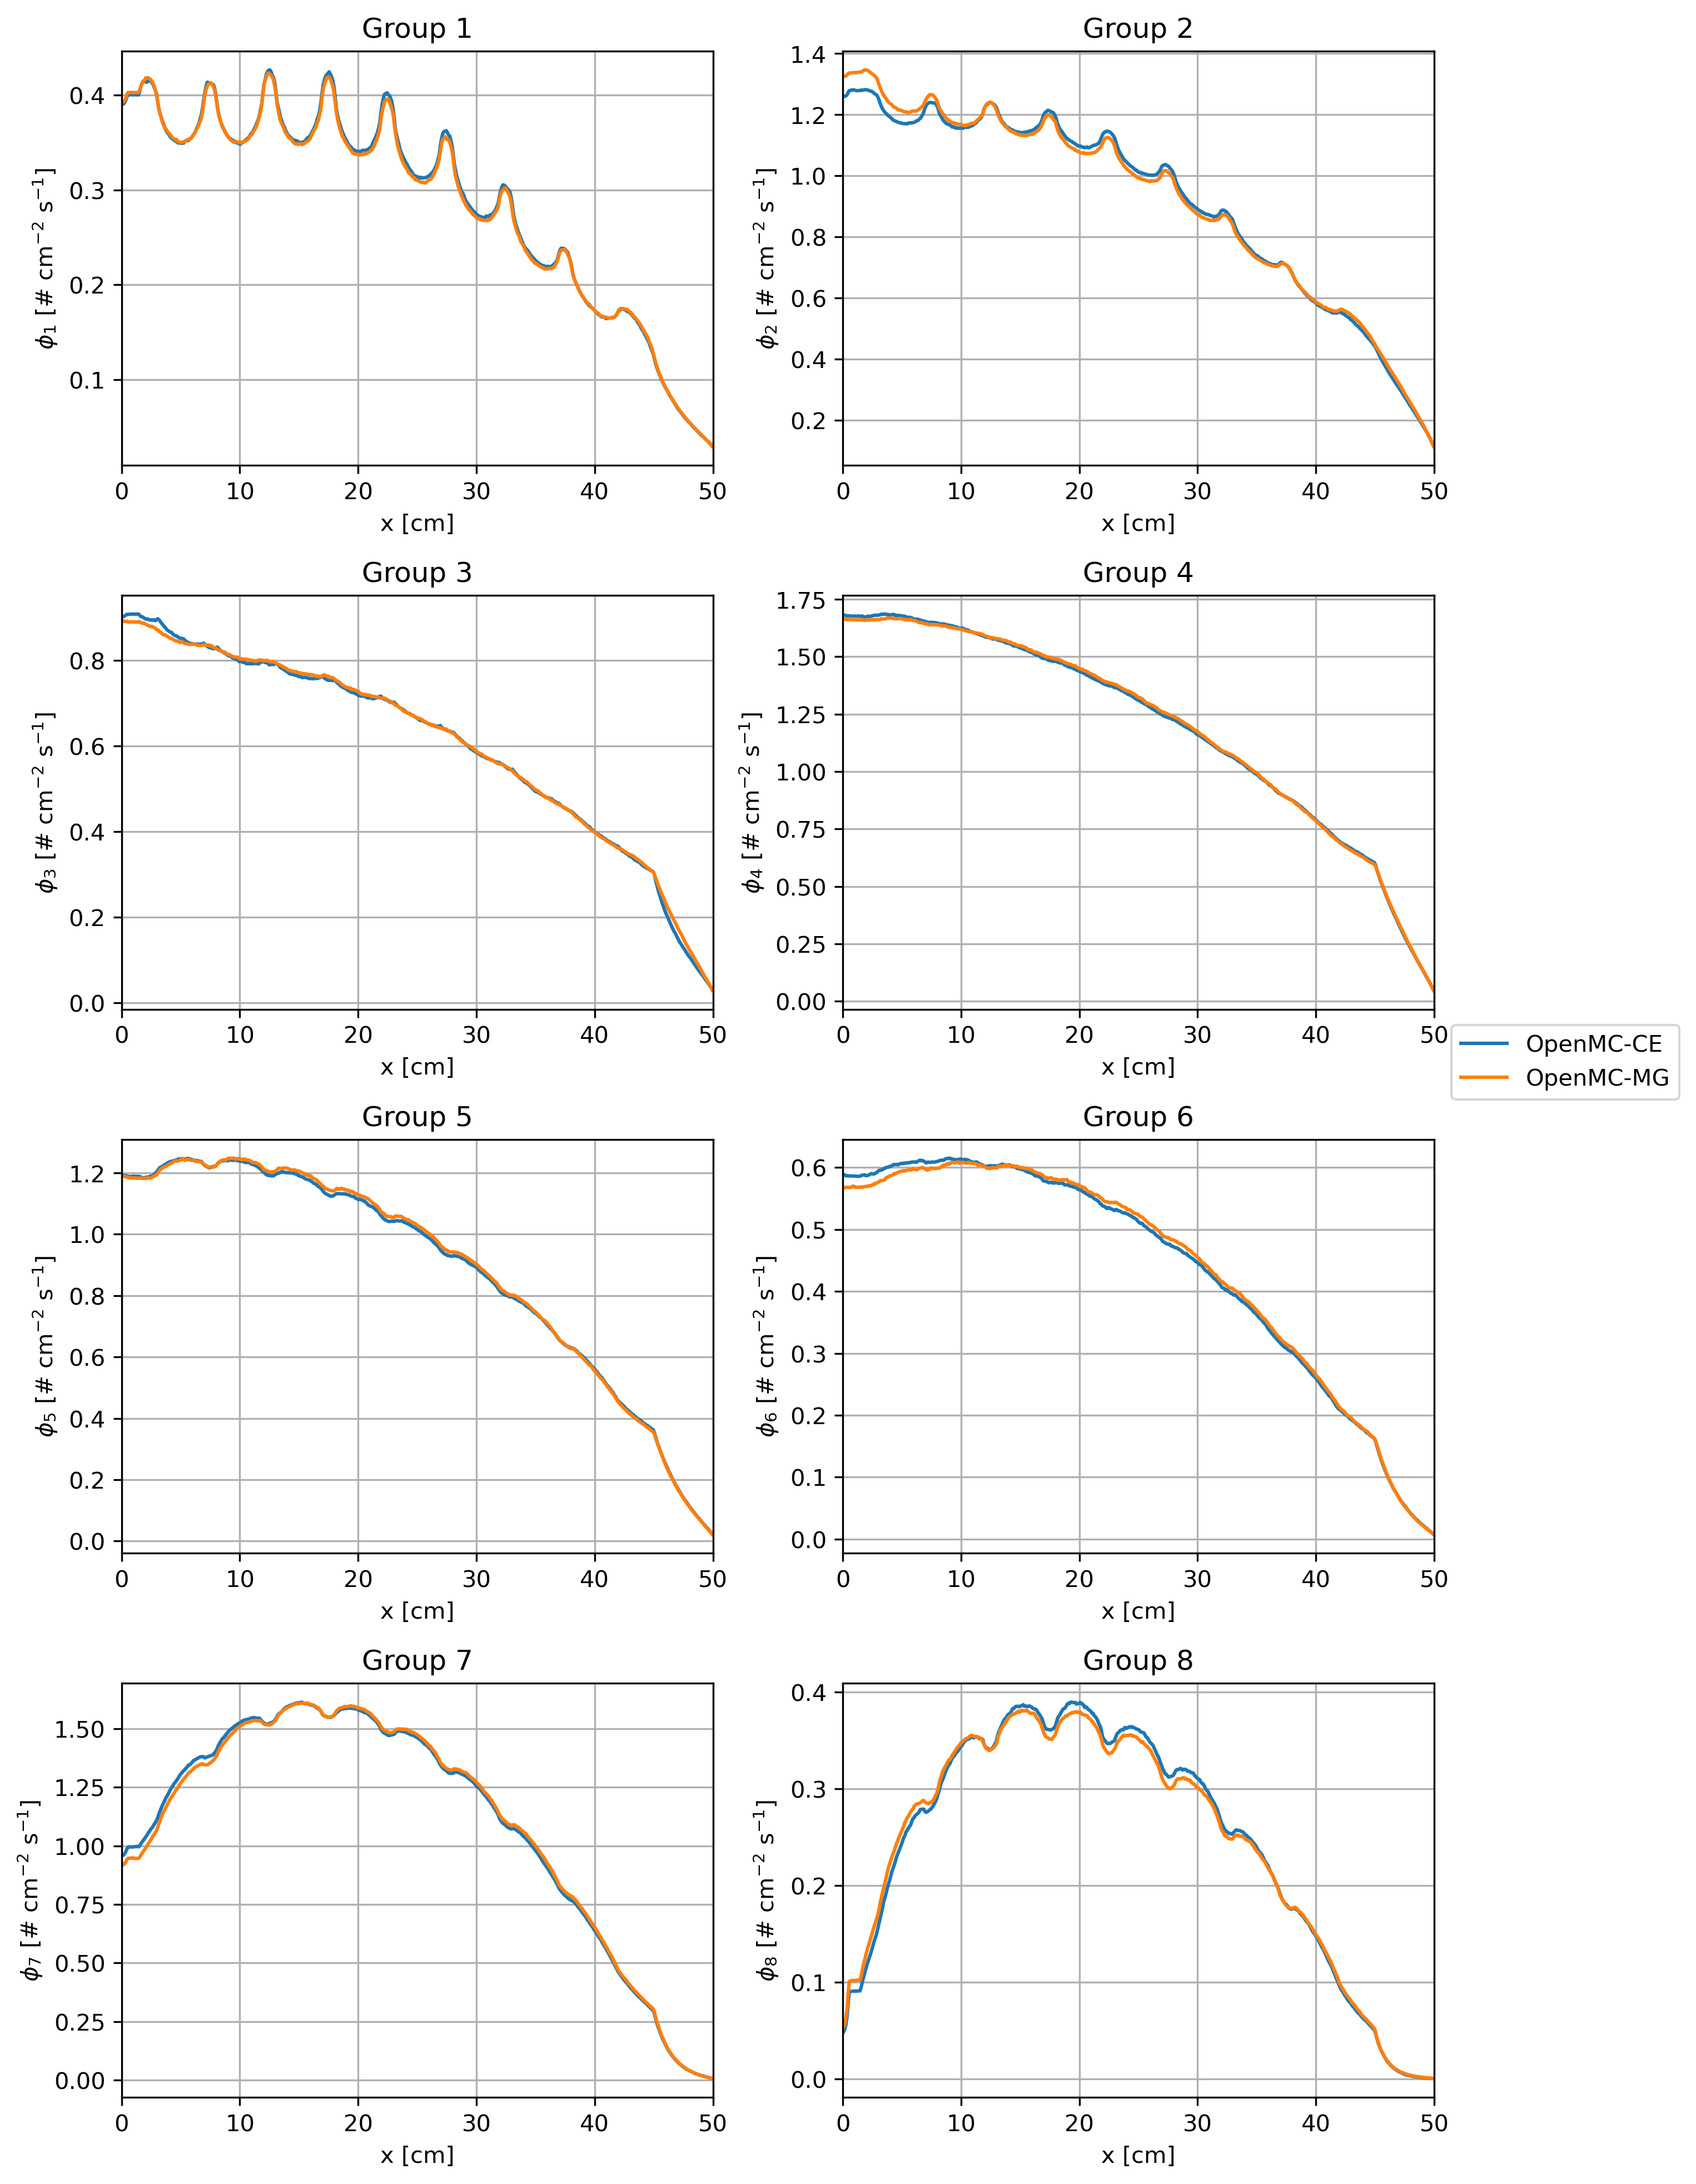
\includegraphics[width=\columnwidth]{case-3b-flux}
  \caption{Case 3b neutron group flux distributions from OpenMC-CE and OpenMC-MG.}
  \label{fig:3b-flux}
\end{figure}

\begin{figure}[htb!]
  \centering
  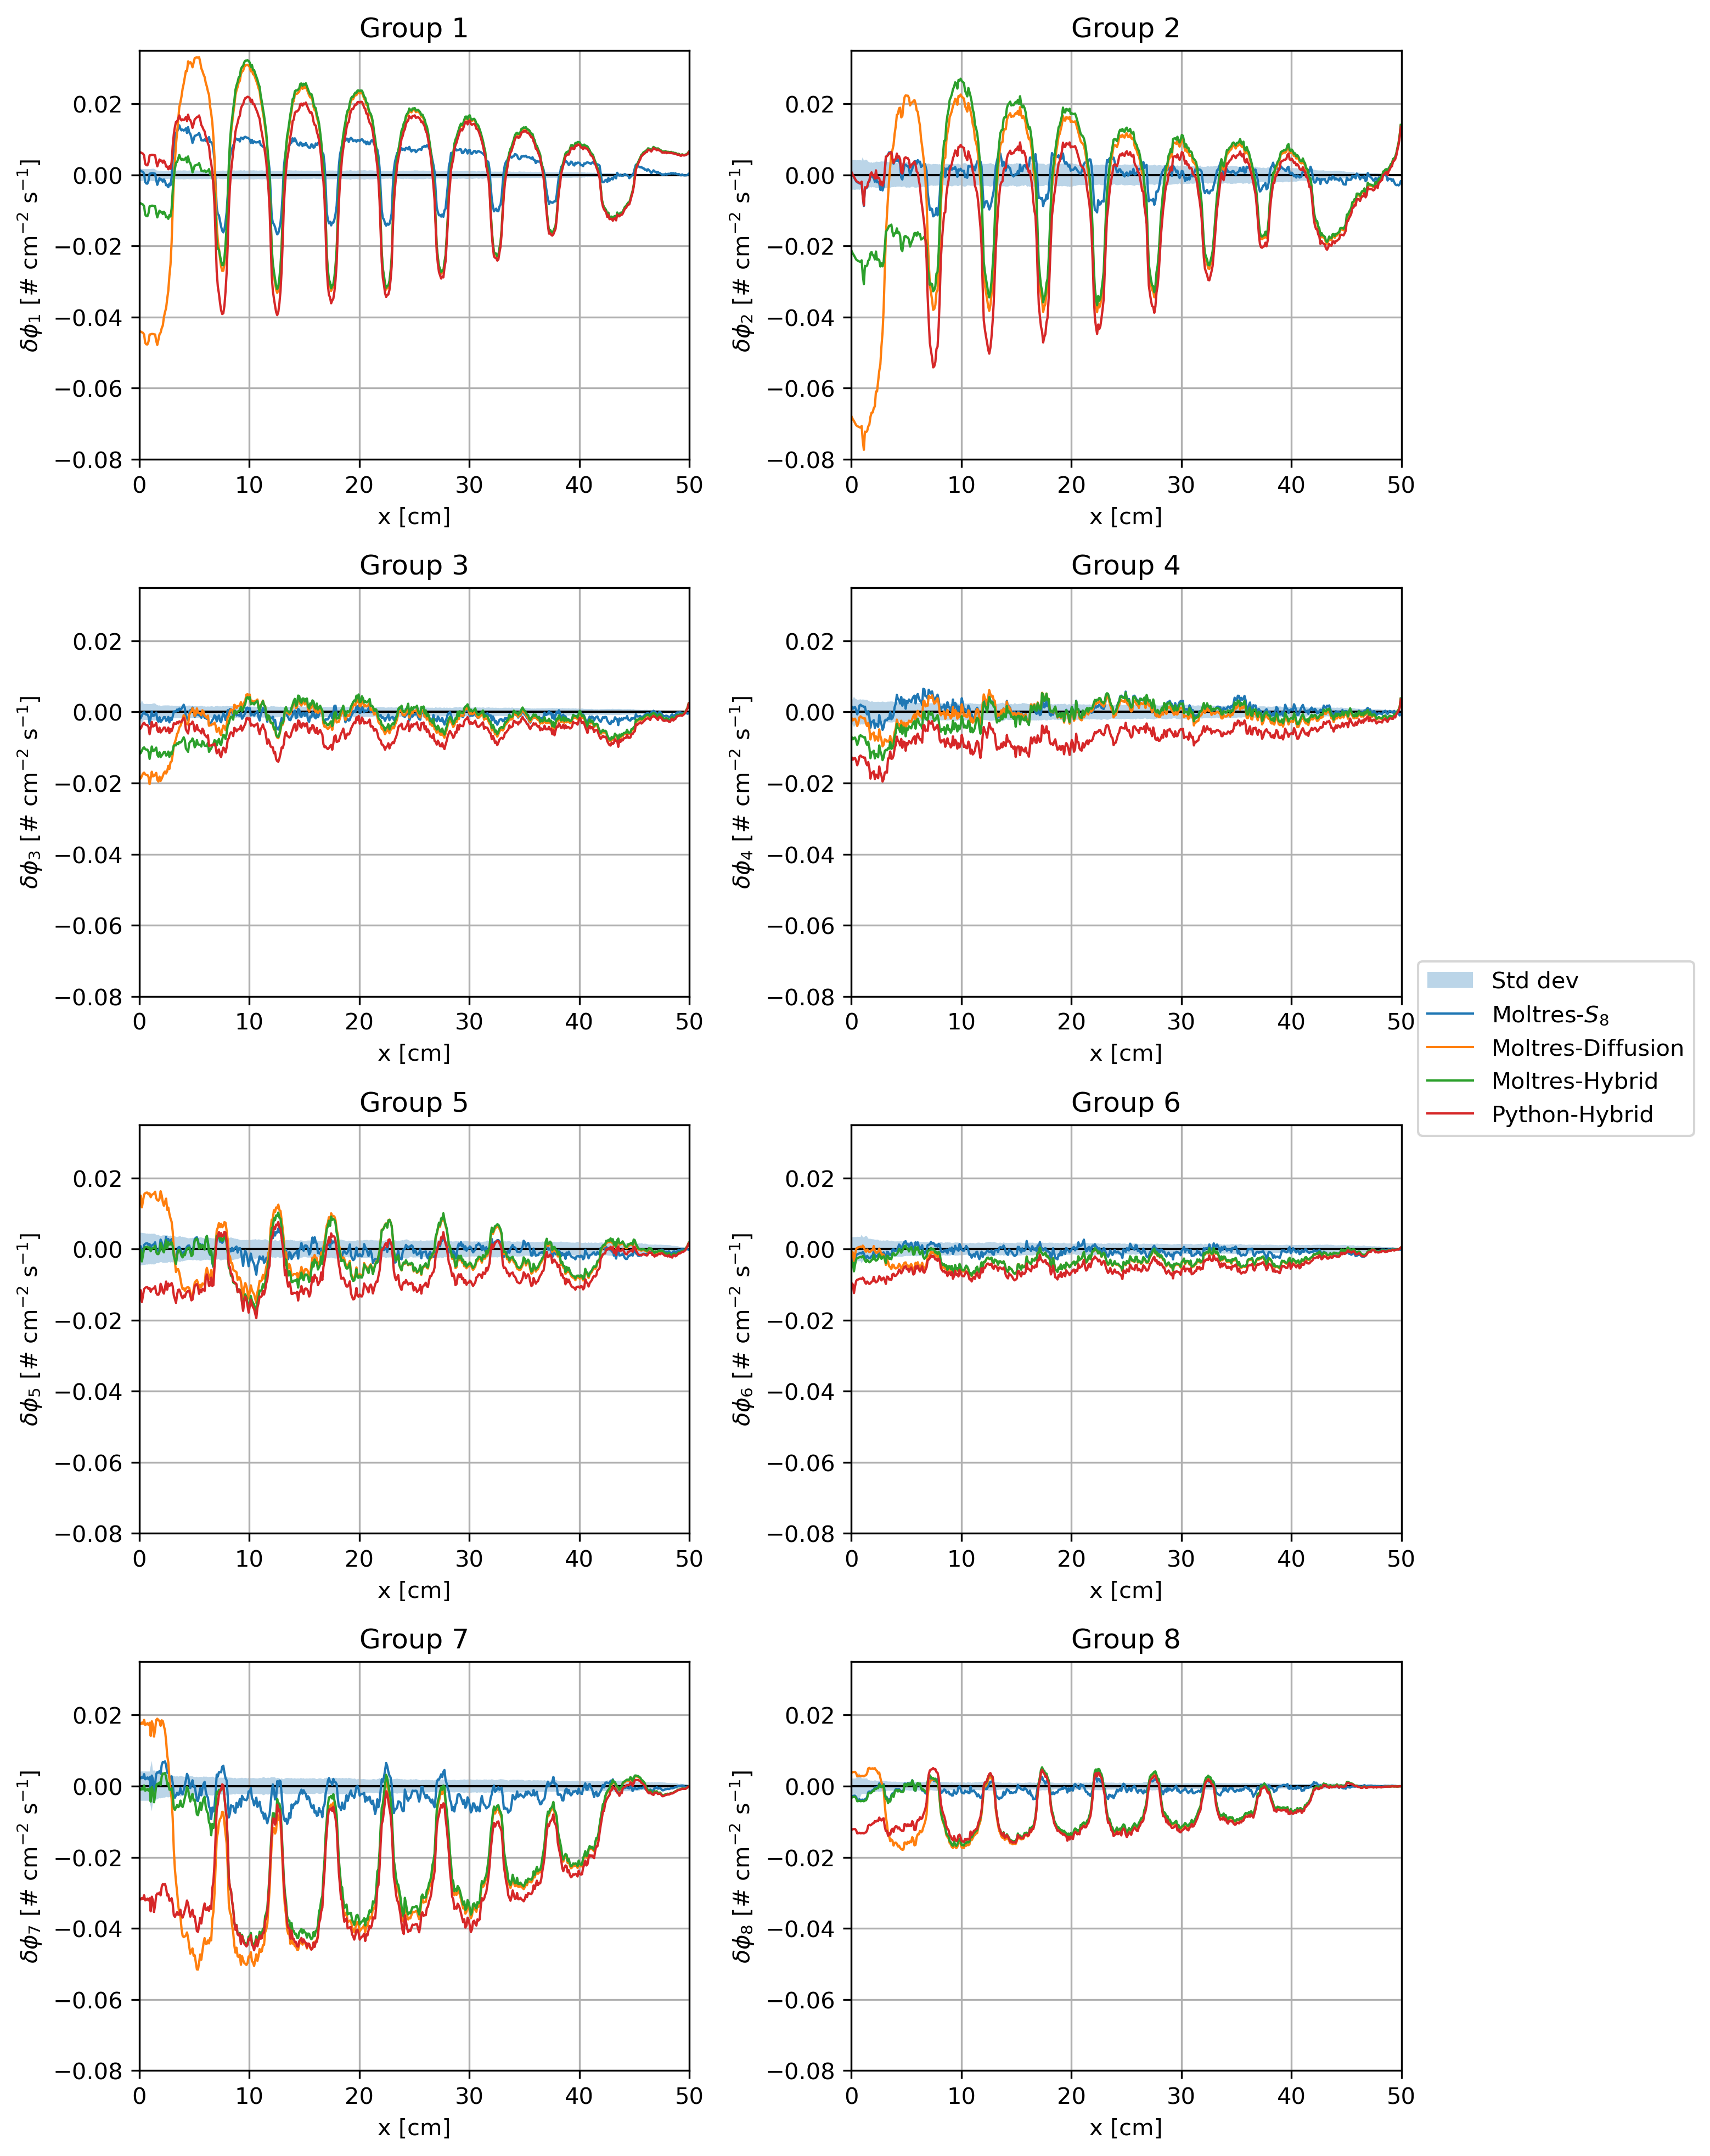
\includegraphics[width=\columnwidth]{case-3a-flux-diff}
  \caption{Absolute difference in neutron group flux distributions for Case 3a from Moltres-$S_8$,
  Moltres-diffusion, Moltres-hybrid, and Python-hybrid relative to OpenMC-MG.}
  \label{fig:3a-flux-diff}
\end{figure}

\begin{figure}[htb!]
  \centering
  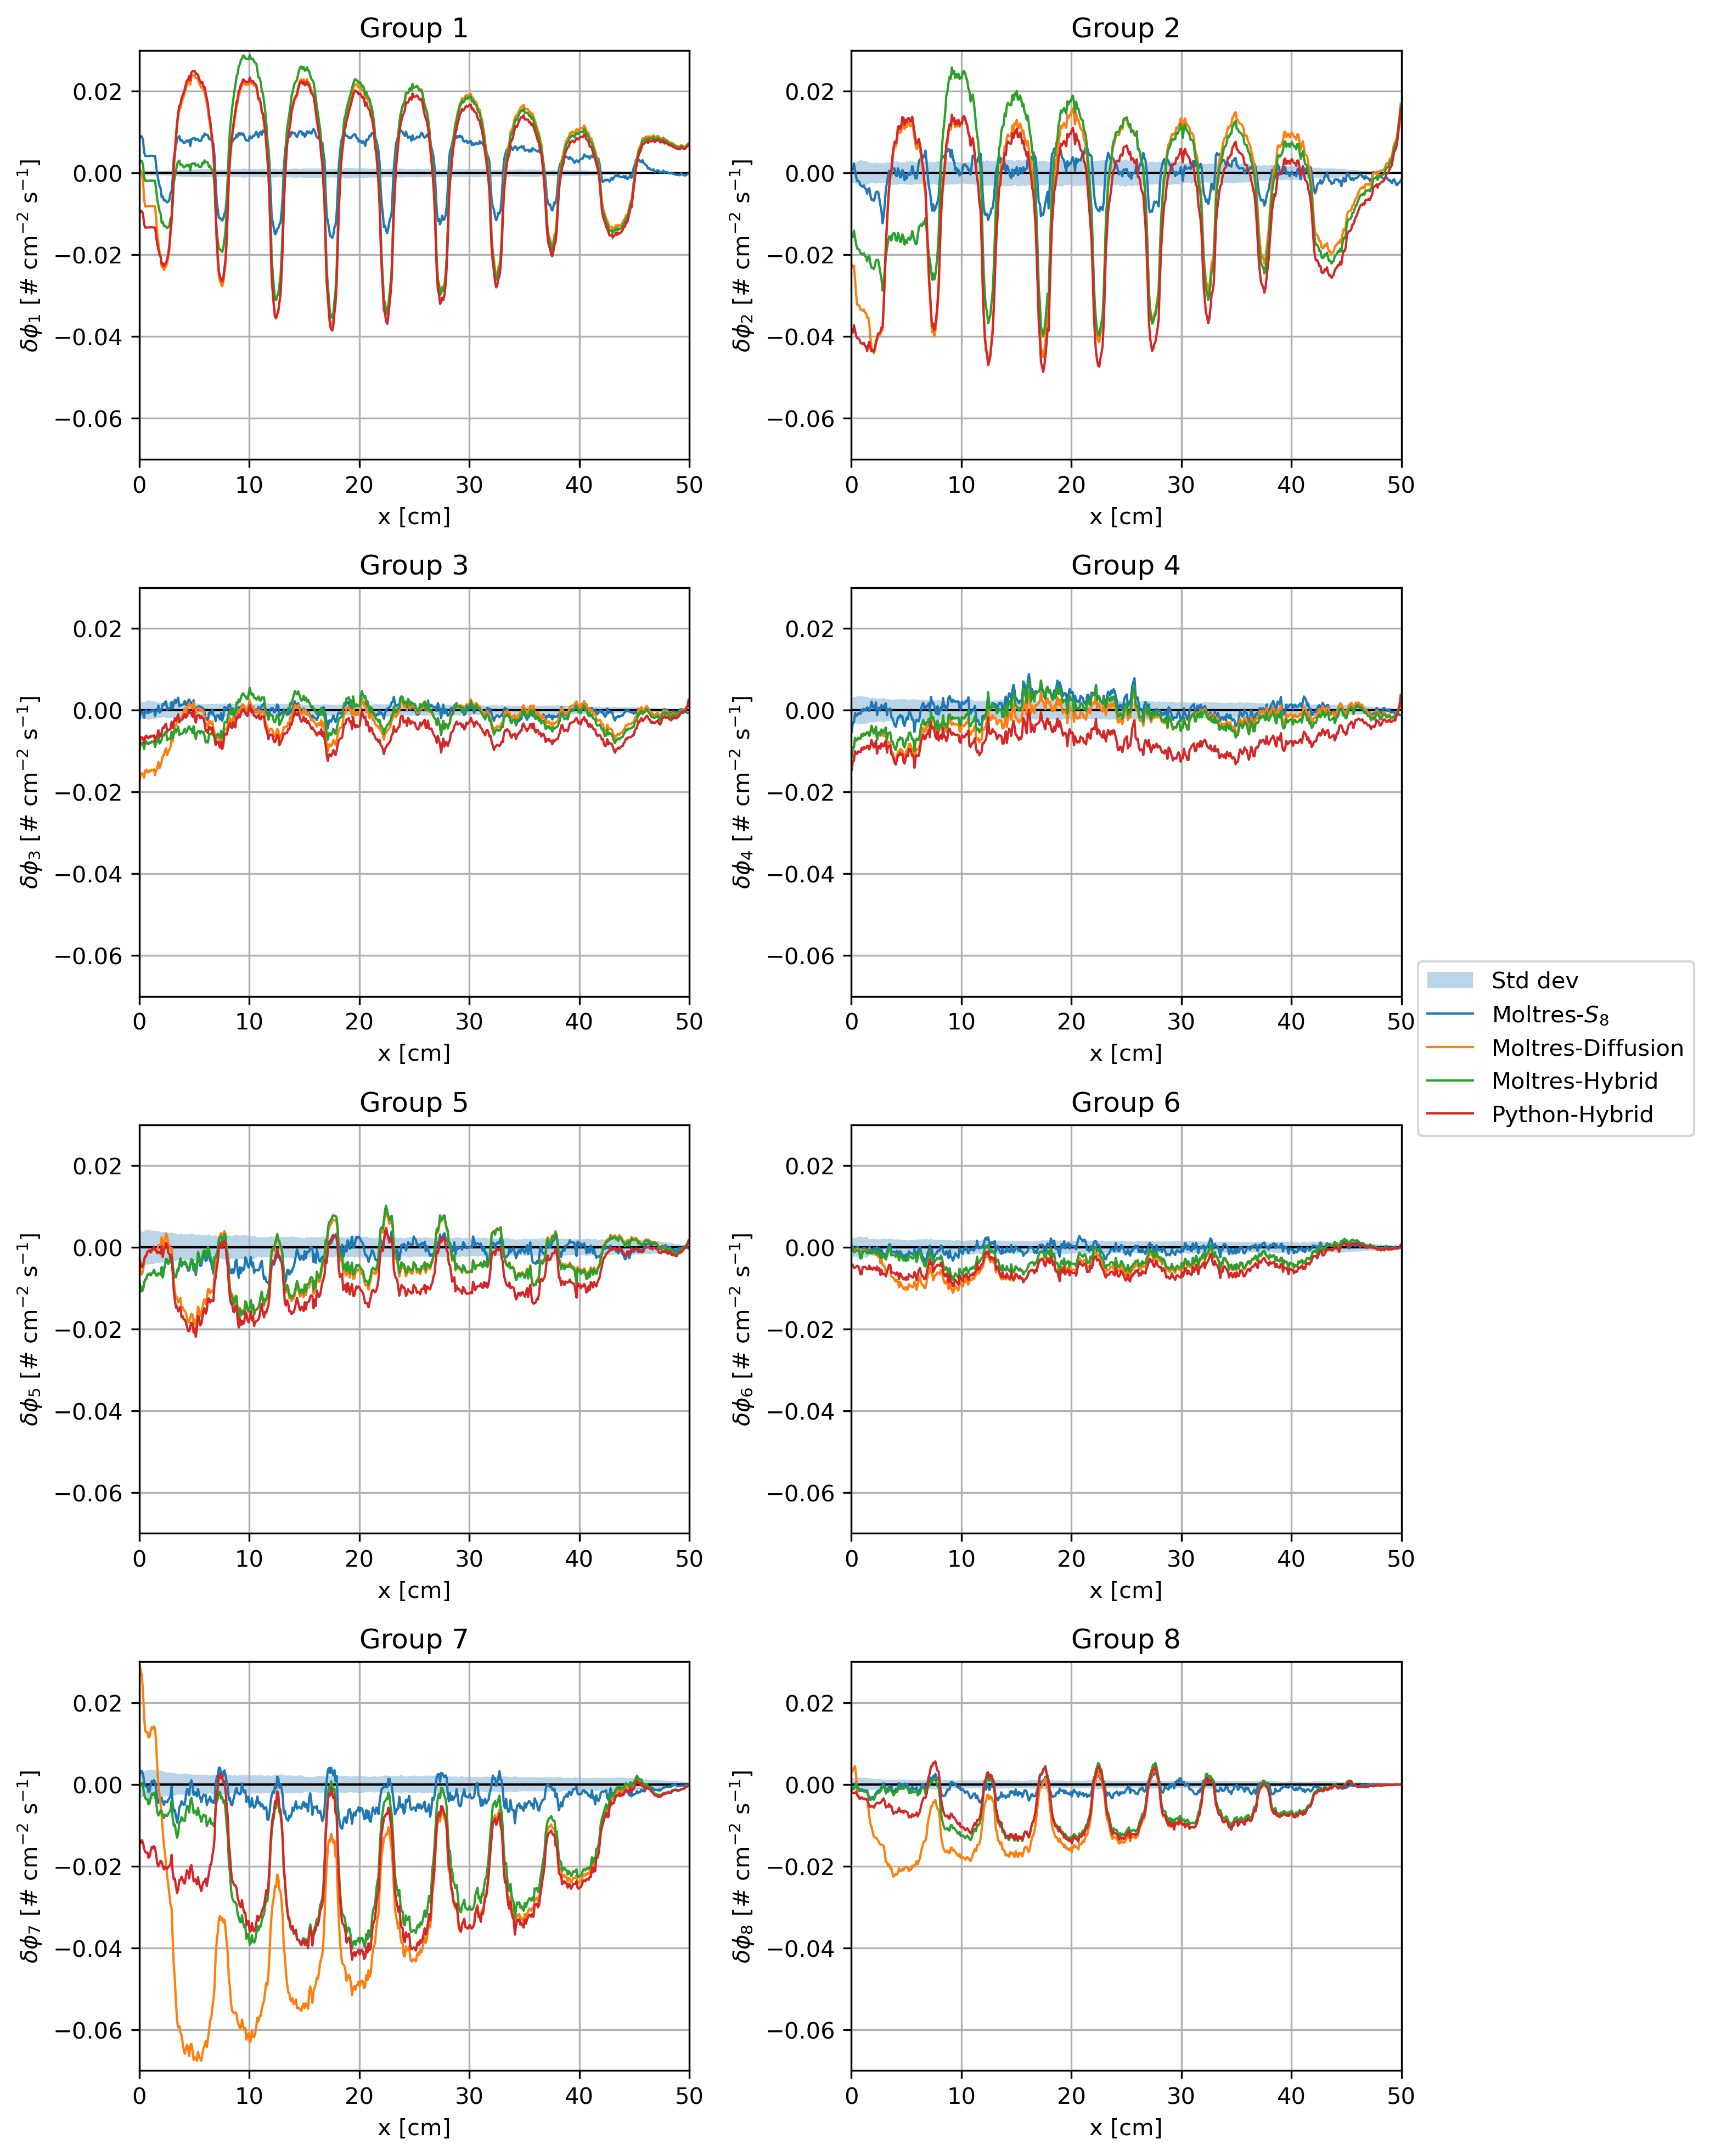
\includegraphics[width=\columnwidth]{case-3b-flux-diff}
  \caption{Absolute difference in neutron group flux distributions for Case 3b from Moltres-$S_8$,
  Moltres-diffusion, Moltres-hybrid, and Python-hybrid relative to OpenMC-MG.}
  \label{fig:3b-flux-diff}
\end{figure}

\FloatBarrier

\subsubsection{Drift \& diffusion correction distribution}

Figures \ref{fig:3b-drift} and \ref{fig:3b-svdc} show the distributions of the drift and diffusion
correction parameters, respectively, in each neutron energy group for Case 3b. As a reminder to the
reader, the hybrid $S_N$-diffusion methods generate these correction parameters in subregions
containing highly neutron absorbing materials. I implemented the drift correction scheme for
Moltres-hybrid and the diffusion correction scheme for Python-hybrid. The hybrid methods
selectively apply the $S_N$ method to improve neutronic modeling within the subregions. I computed
the reference distributions (yellow data points) in both plots from reference flux solutions of the
standard $S_8$ method.

As discussed in Section \ref{sec:buffer-region}, both sets of correction parameters generated by
the two correction schemes match their respective reference values within the correction subregion
from $x=0$ cm to 10 cm except near the subregion boundary at $x=10$ cm. Therefore, both schemes
provide improved flux estimates in the subregion compared to the neutron diffusion method.
The prior reactivity and flux distribution results indicate Moltres-hybrid is more accurate
than Python-hybrid relative to OpenMC-MG as the reference.

In Figure \ref{fig:3b-drift}, the drift
correction distributions (Moltres-hybrid) for all eight energy groups are well-defined throughout
the subregion and are continuous except at material interfaces. Consequently, the drift correction
scheme provides accurate flux corrections for about 75\% of the subregion based on the buffer
region cutoff criteria which occurs around $x=7.5$ cm where most of the drift distributions are
zero (refer to Section \ref{sec:buffer-region}). By contrast, the diffusion correction
distributions in Figure \ref{fig:3b-svdc} contains numerous discontinuities tending towards
positive or negative infinity in all eight energy groups. The discontinuities arise when
computing corrected diffusion coefficients (Eq. \ref{eq:svdc}) near flux peaks and troughs
(stationary points) where the flux gradients approach zero. The location of stationary points from
the diffusion and $S_N$ calculations in the hybrid method do not necessarily coincide, resulting in
discontinuous flux gradients in the final flux solution. Discontinuities are generally unavoidable
in most problems because the fluxes typically reach local minima in control rod regions.
Furthermore, unlike negative drift coefficients, negative diffusion coefficients are unphysical.
Taking everything into consideration, the diffusion correction scheme is less accurate and more
numerically unstable than the drift correction scheme.

The subsequent discussions on the correction region size and the number of outer
iterations focus on the drift correction scheme of the hybrid method.

\begin{figure}[htb!]
  \centering
  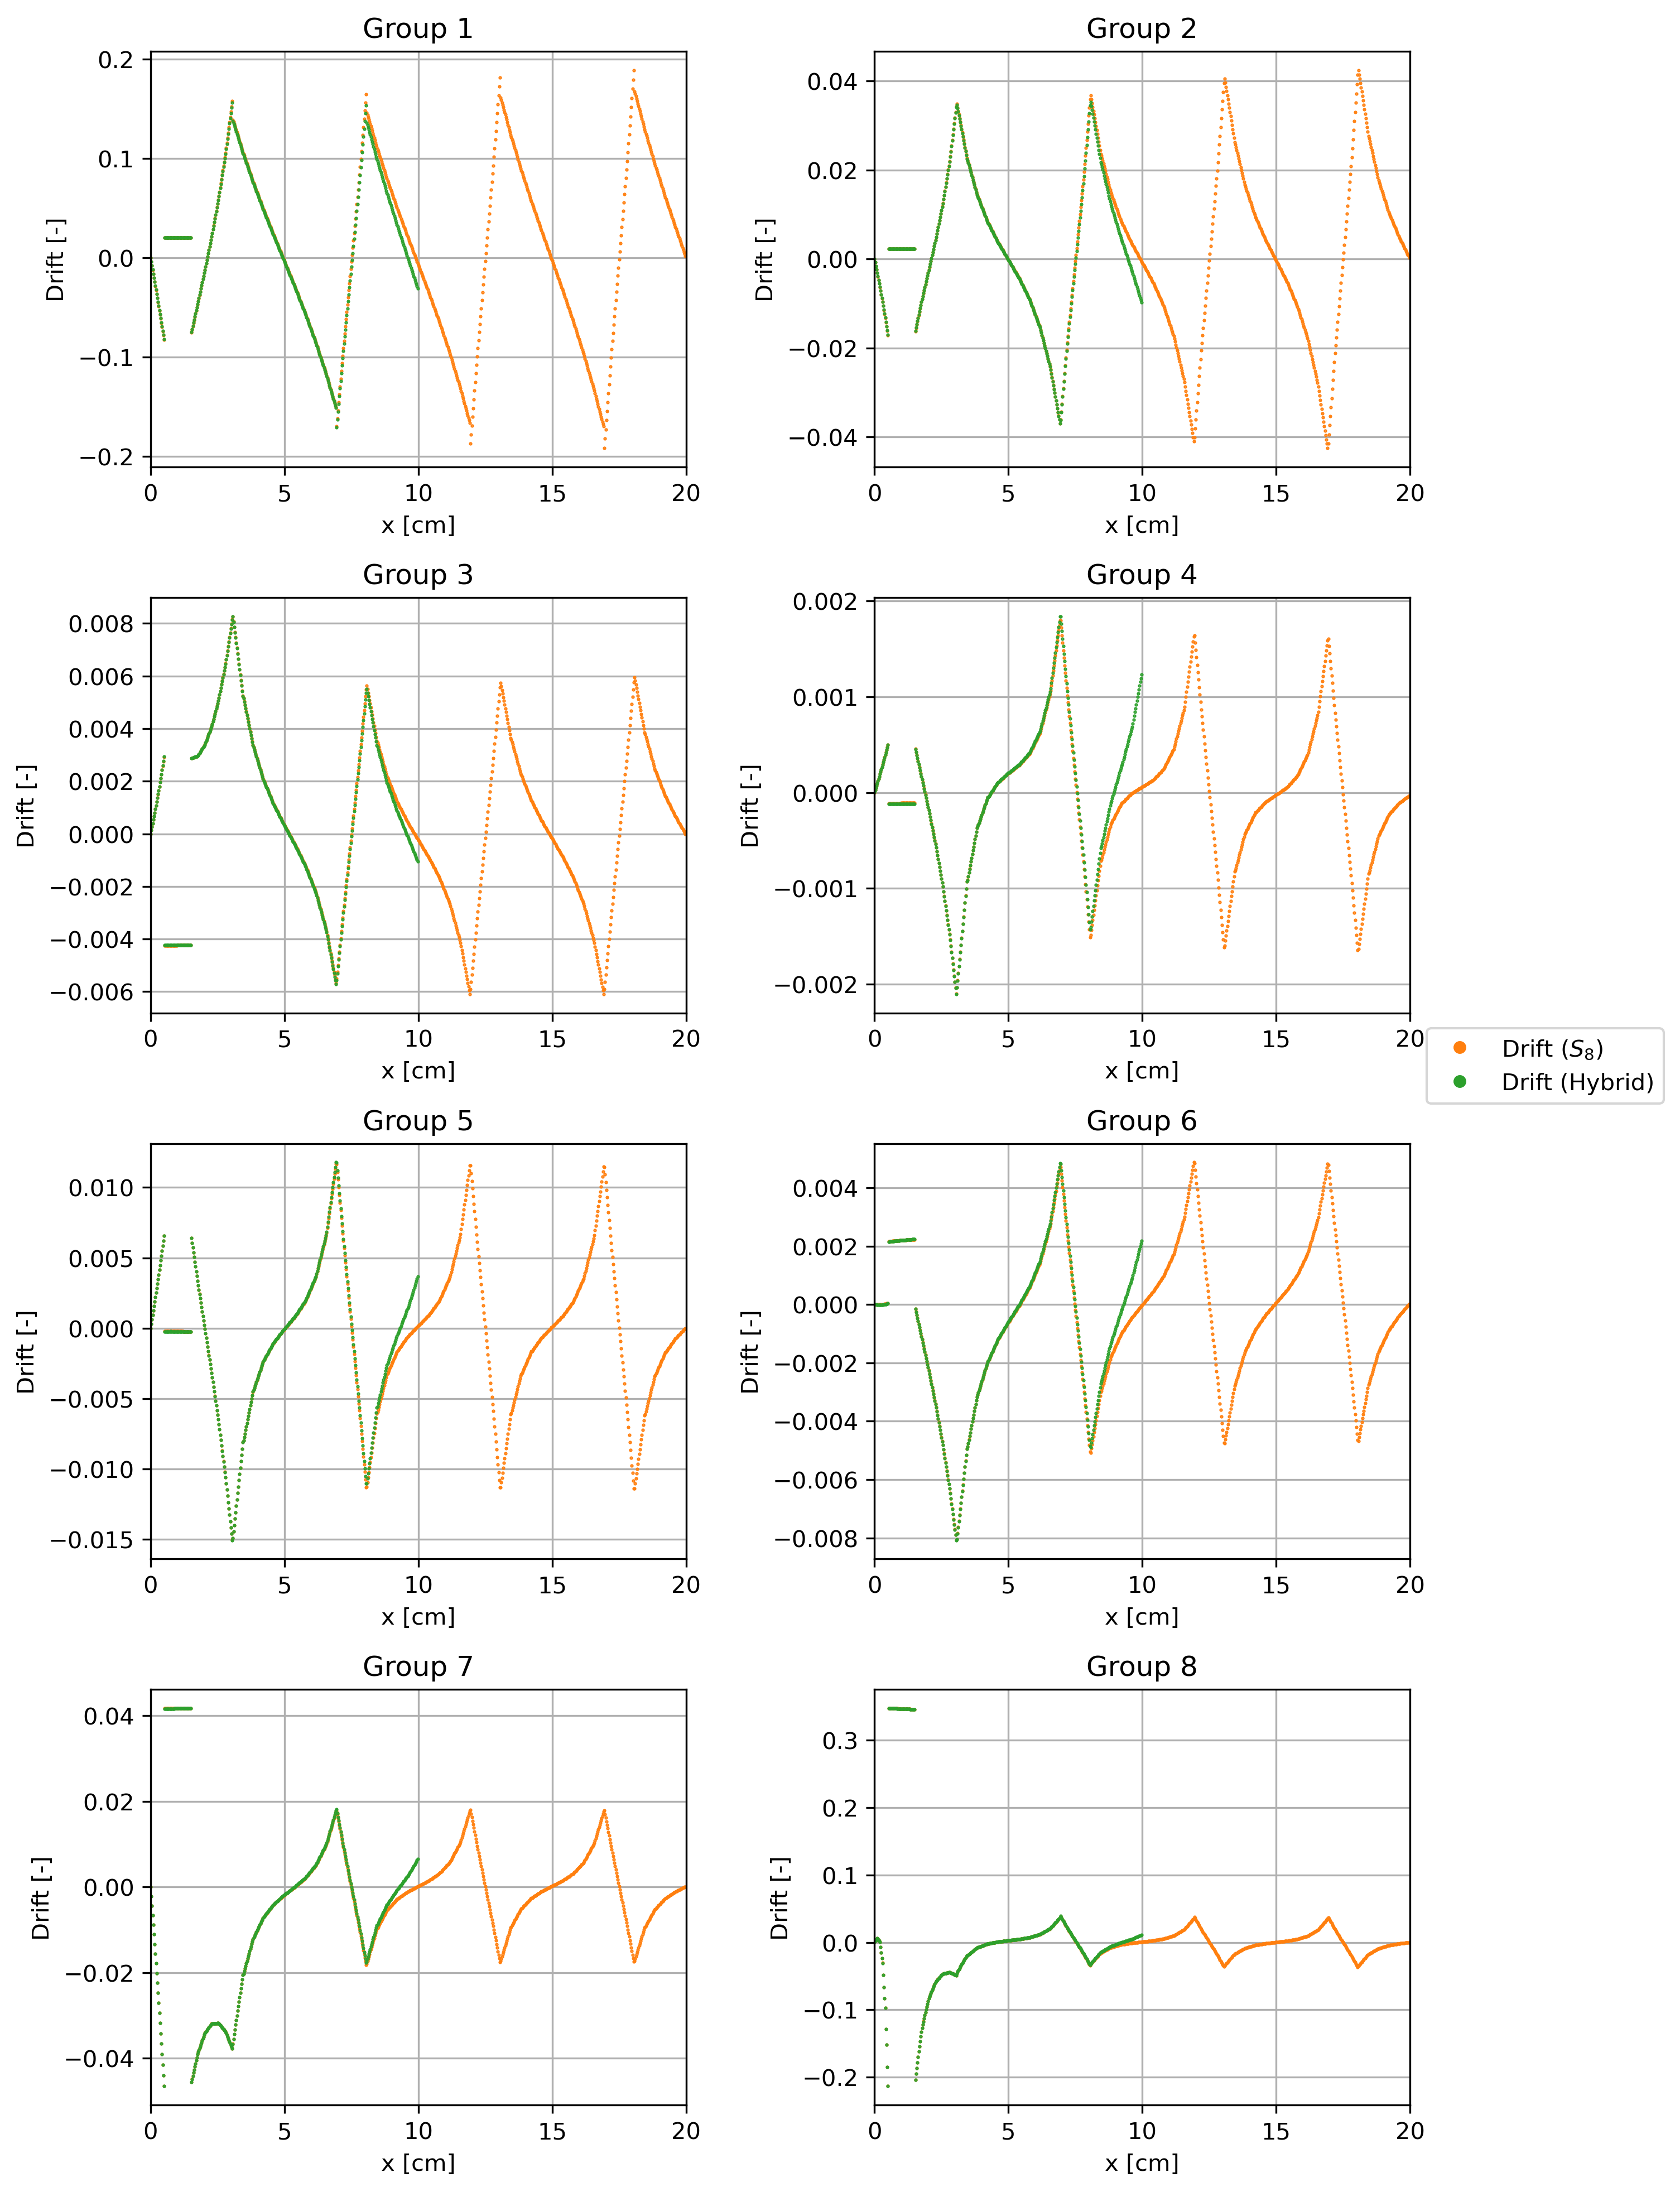
\includegraphics[width=\columnwidth]{case-3b-drift}
  \caption{Multigroup drift correction ($\vec{D}_g$) $x$-component distributions from the
  Moltres-hybrid and Moltres-$S_8$ solvers.}
  \label{fig:3b-drift}
\end{figure}

\begin{figure}[htb!]
  \centering
  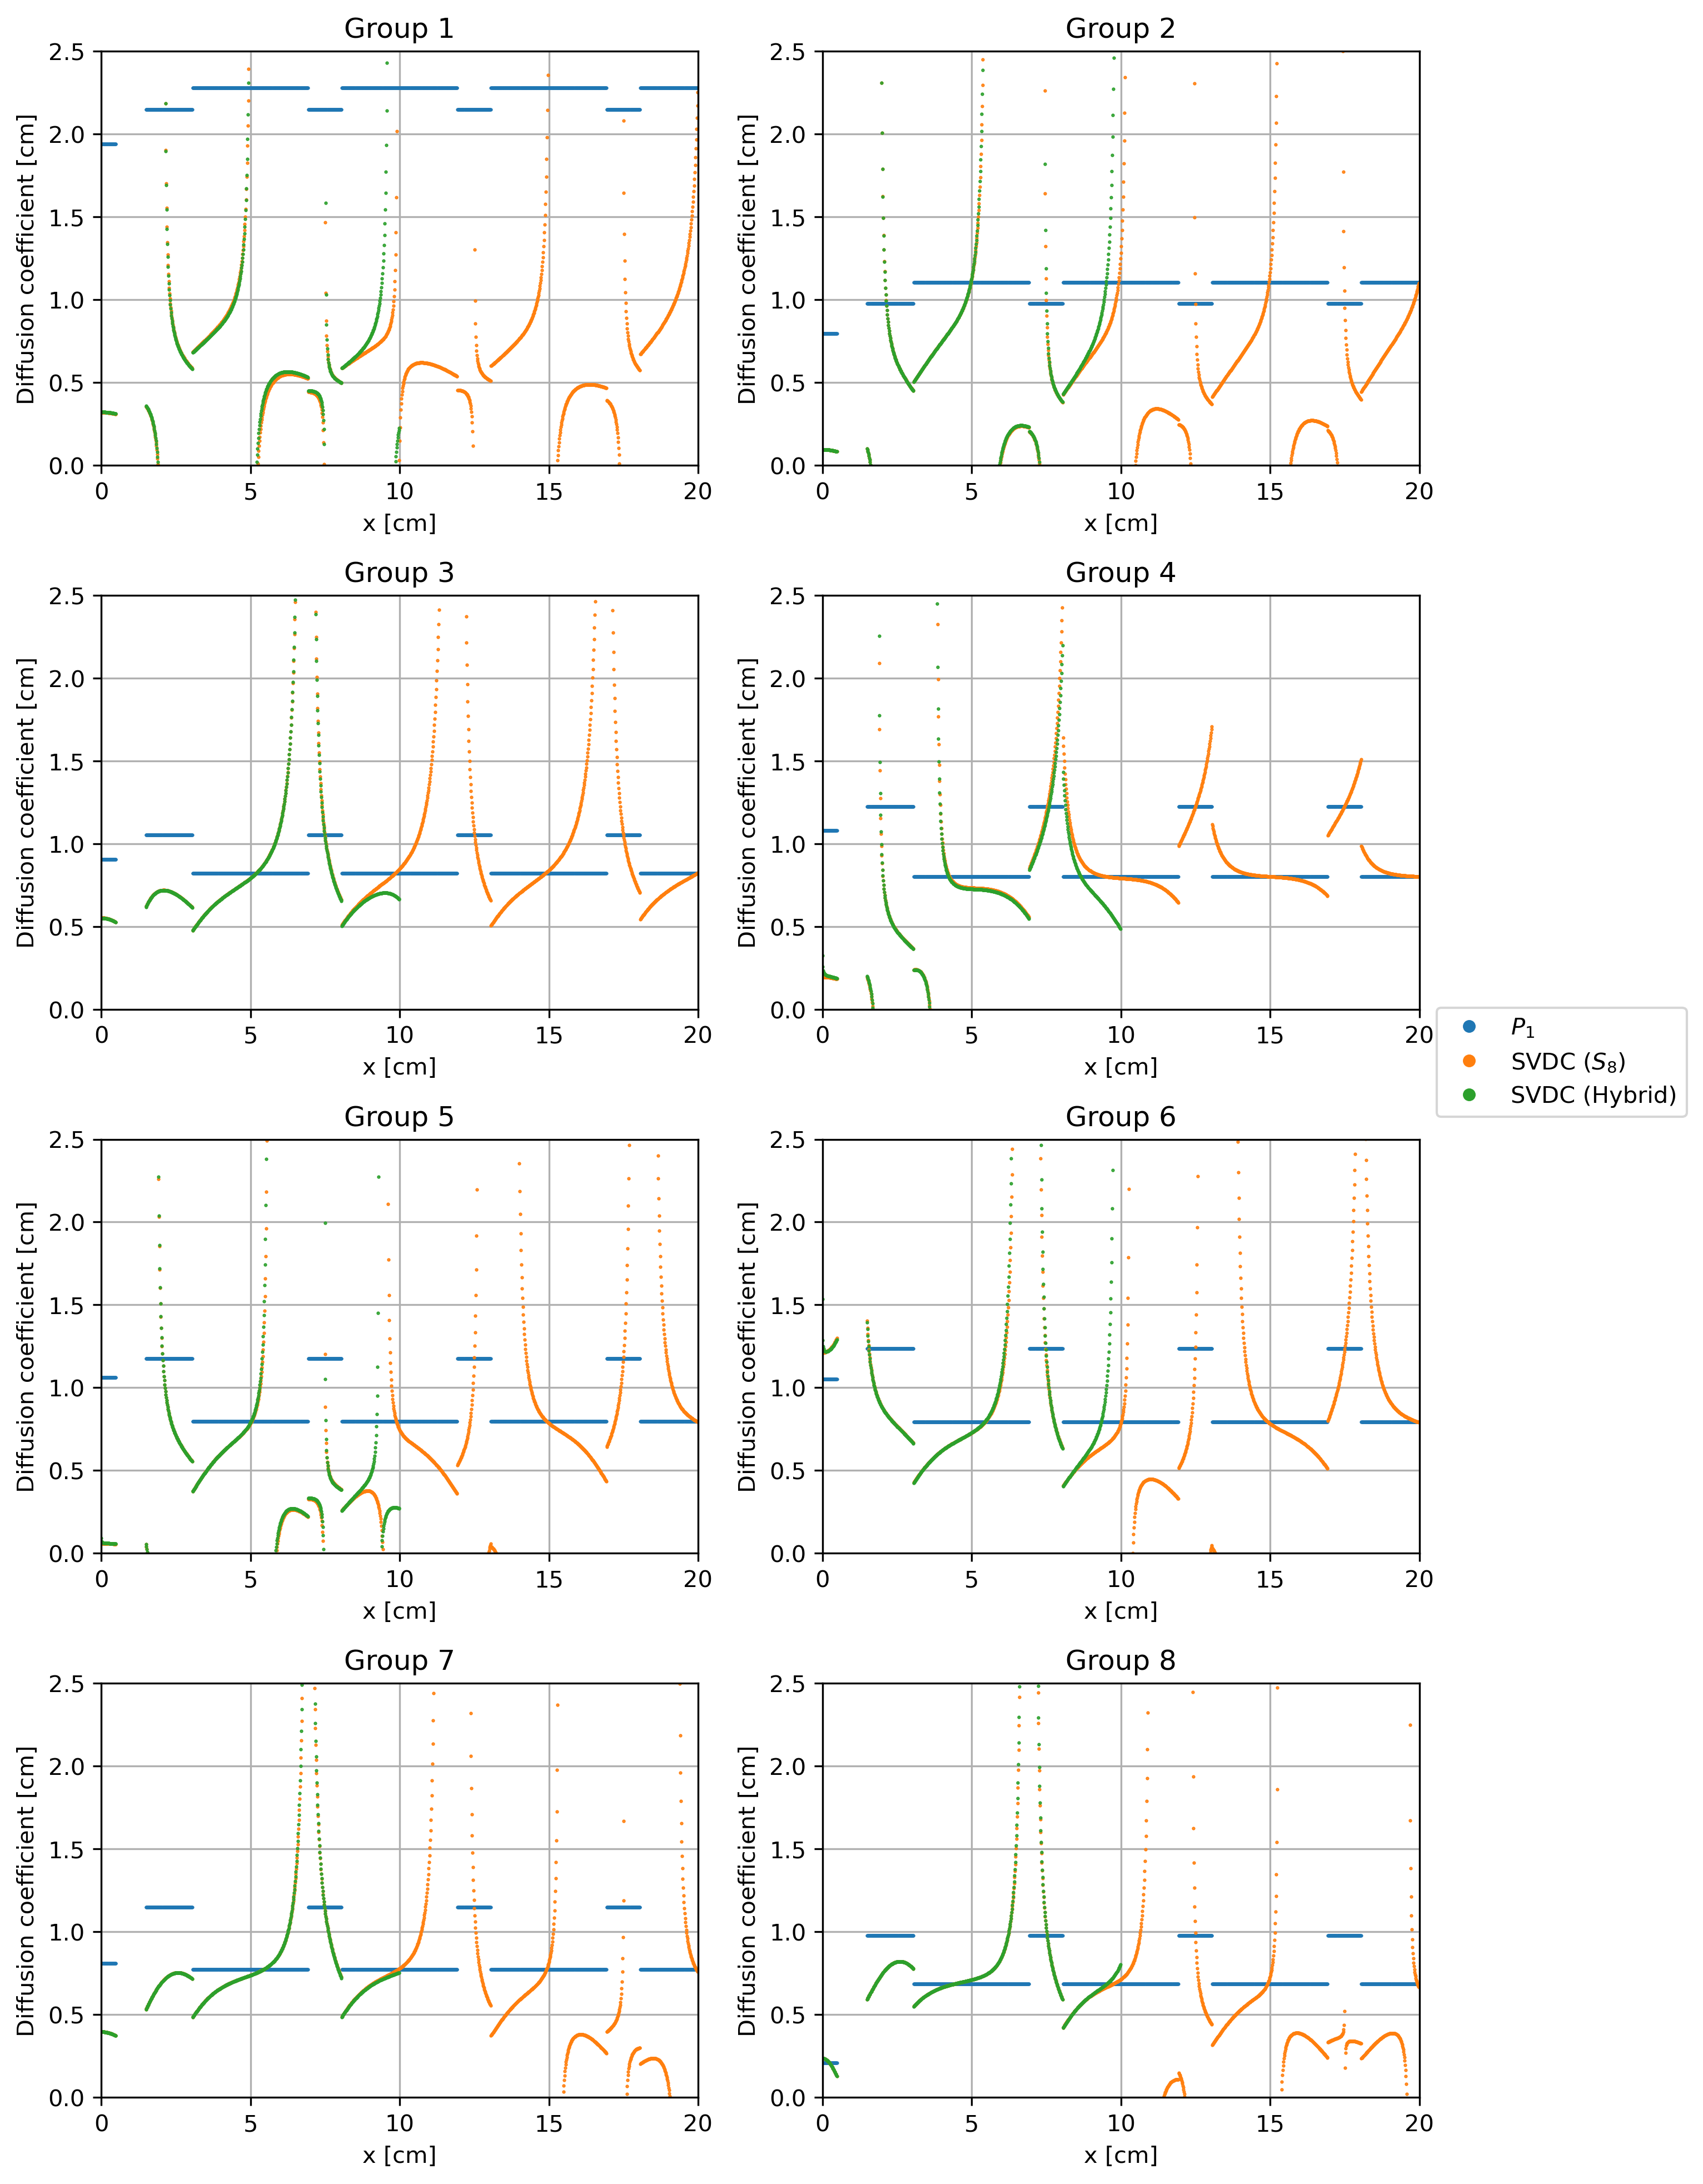
\includegraphics[width=\columnwidth]{case-3b-svdc}
  \caption{Multigroup diffusion correction ($D^s_g$) $x$-component distributions from the
    Python-hybrid and Python-$S_8$ solvers.}
  \label{fig:3b-svdc}
\end{figure}

\FloatBarrier

\subsubsection{Impact of correction subregion sizes}

The hybrid $S_N$-diffusion method relies on $S_N$ calculations in the correction subregion to
generate flux corrections. Minimizing the size of the correction subregion and the $S_N$ subproblem
is essential for the hybrid method to be computationally competitive for time-dependent full-core
simulations. I investigated the effect of the correction subregion size on the $k_\text{eff}$ and
control rod worth estimates with Cases 3a and 3b by varying the subregion sizes from 10 cm to 40 cm
at 5 cm-intervals.

Figures \ref{fig:v1-size-a-k} and \ref{fig:v1-size-b-k} show the $k_\text{eff}$ estimates from the
hybrid method for Cases 3a and 3b, respectively. In both cases, the $k_\text{eff}$ values initially
decrease as the correction subregion sizes increase before reversing in trend when the subregion
size reaches 35 cm and beyond. The $k_\text{eff}$ values vary by up to 164 pcm for Case 3a and 109
pcm for Case 3b. An important observation here is that the $k_\text{eff}$ values do not
monotonically converge towards the $k_\text{eff}$ estimate from the $S_8$ method. The data implies
other significant sources of discrepancies exist beyond those being corrected in the
correction subregion by the hybrid method.

% In general,
% discrepancies arise between the neutron diffusion method and $S_8$ from the neutron diffusion 
% method's failure to accurately model the neutron flux in the fuel-graphite lattice region. The
% figures imply that those discrepancies result in a positive change in $k_\text{eff}$ since the
% $k_\text{eff}$ decreases as larger fractions of the problem domain benefit from flux corrections.
% The remaining discrepancy in $k_\text{eff}$ between the hybrid method with a correction subregion
% size of 40 cm and the $S_8$ method arises from 

\begin{figure}[htb!]
  \centering
  \begin{subfigure}[b]{0.49\columnwidth}
    \centering
    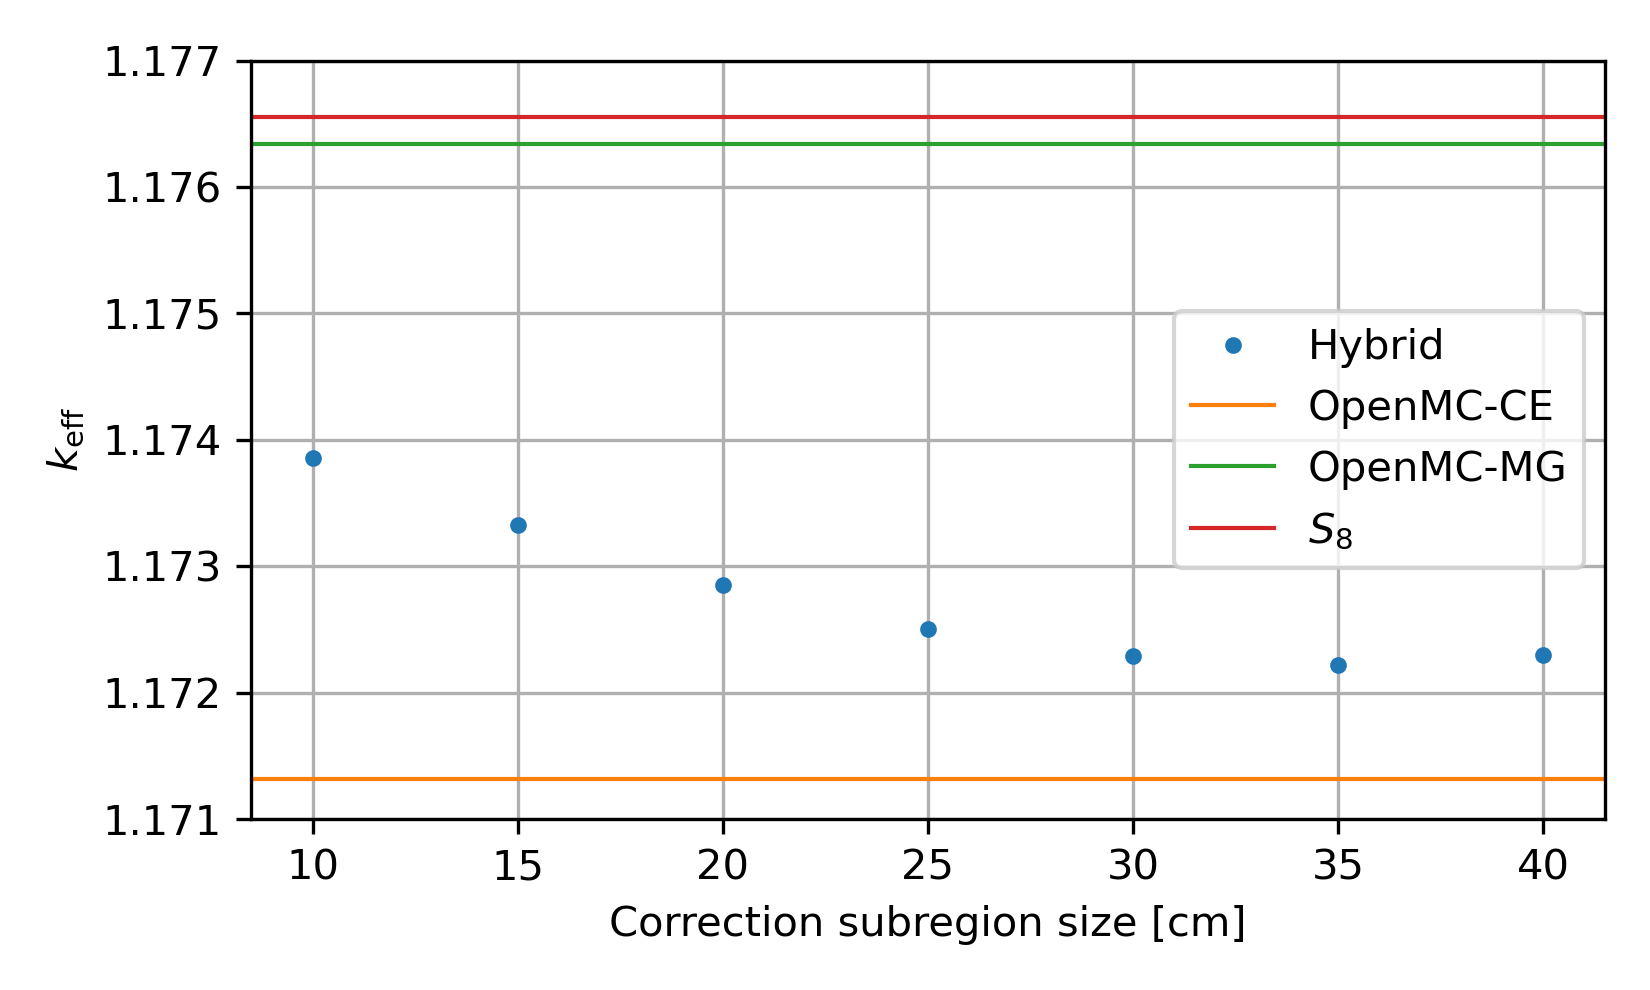
\includegraphics[width=\columnwidth]{correction-size-a-k}
    \caption{Case 3a}
    \label{fig:v1-size-a-k}
  \end{subfigure}
  \hfill
  \begin{subfigure}[b]{0.49\columnwidth}
    \centering
    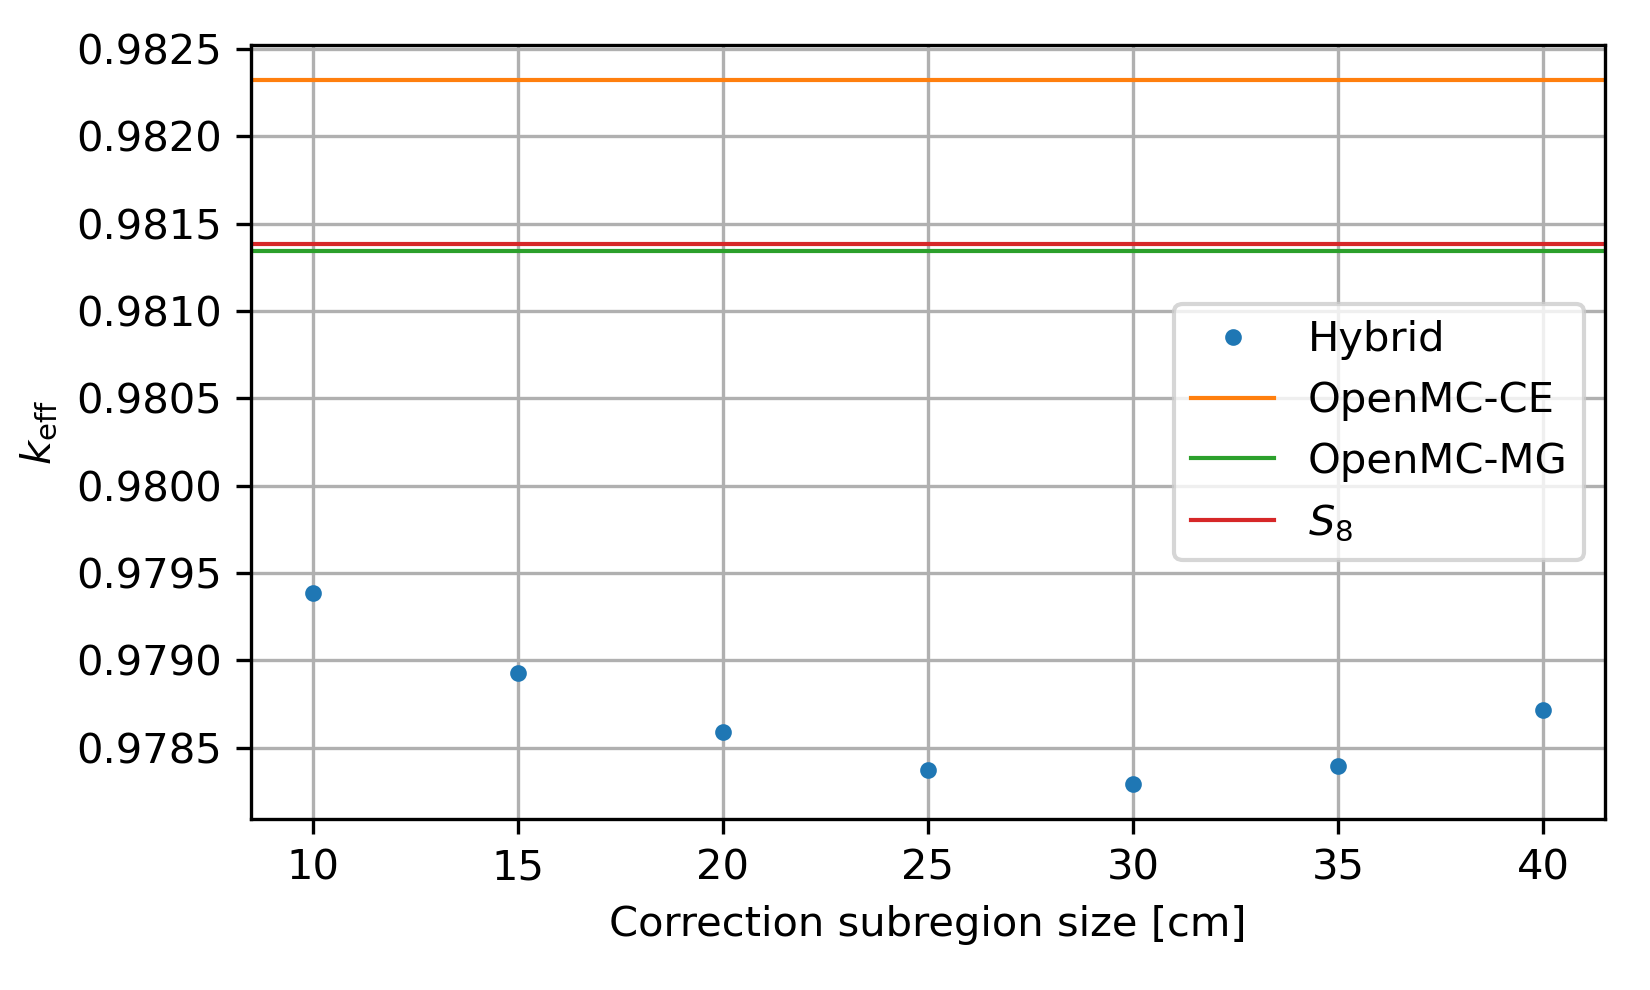
\includegraphics[width=\columnwidth]{correction-size-b-k}
    \caption{Case 3b}
    \label{fig:v1-size-b-k}
  \end{subfigure}
  \caption{$k_\text{eff}$ estimates from the hybrid method for Cases 3a and 3b with different
  correction subregion sizes. The horizontal lines indicate $k_\text{eff}$ estimates from the
  OpenMC-CE, OpenMC-MG, and $S_8$ methods.}
  \label{fig:v1-size-k}
\end{figure}

Figure \ref{fig:v1-size-rho} shows the percentage difference in rod worth relative to OpenMC-CE. 
Due to the identical trends observed in the $k_\text{eff}$ estimates of both cases, the control rod
worth estimates do not change significantly when the correction subregion
sizes change. This indicates limiting the correction subregion size to save
computational cost on the expensive $S_N$ calculations has a negligible impact on rod worth
estimates. The rod worth estimates for all investigated correction subregion sizes remain within
0.2\% of the $S_8$ method.

\begin{figure}[htb!]
  \centering
  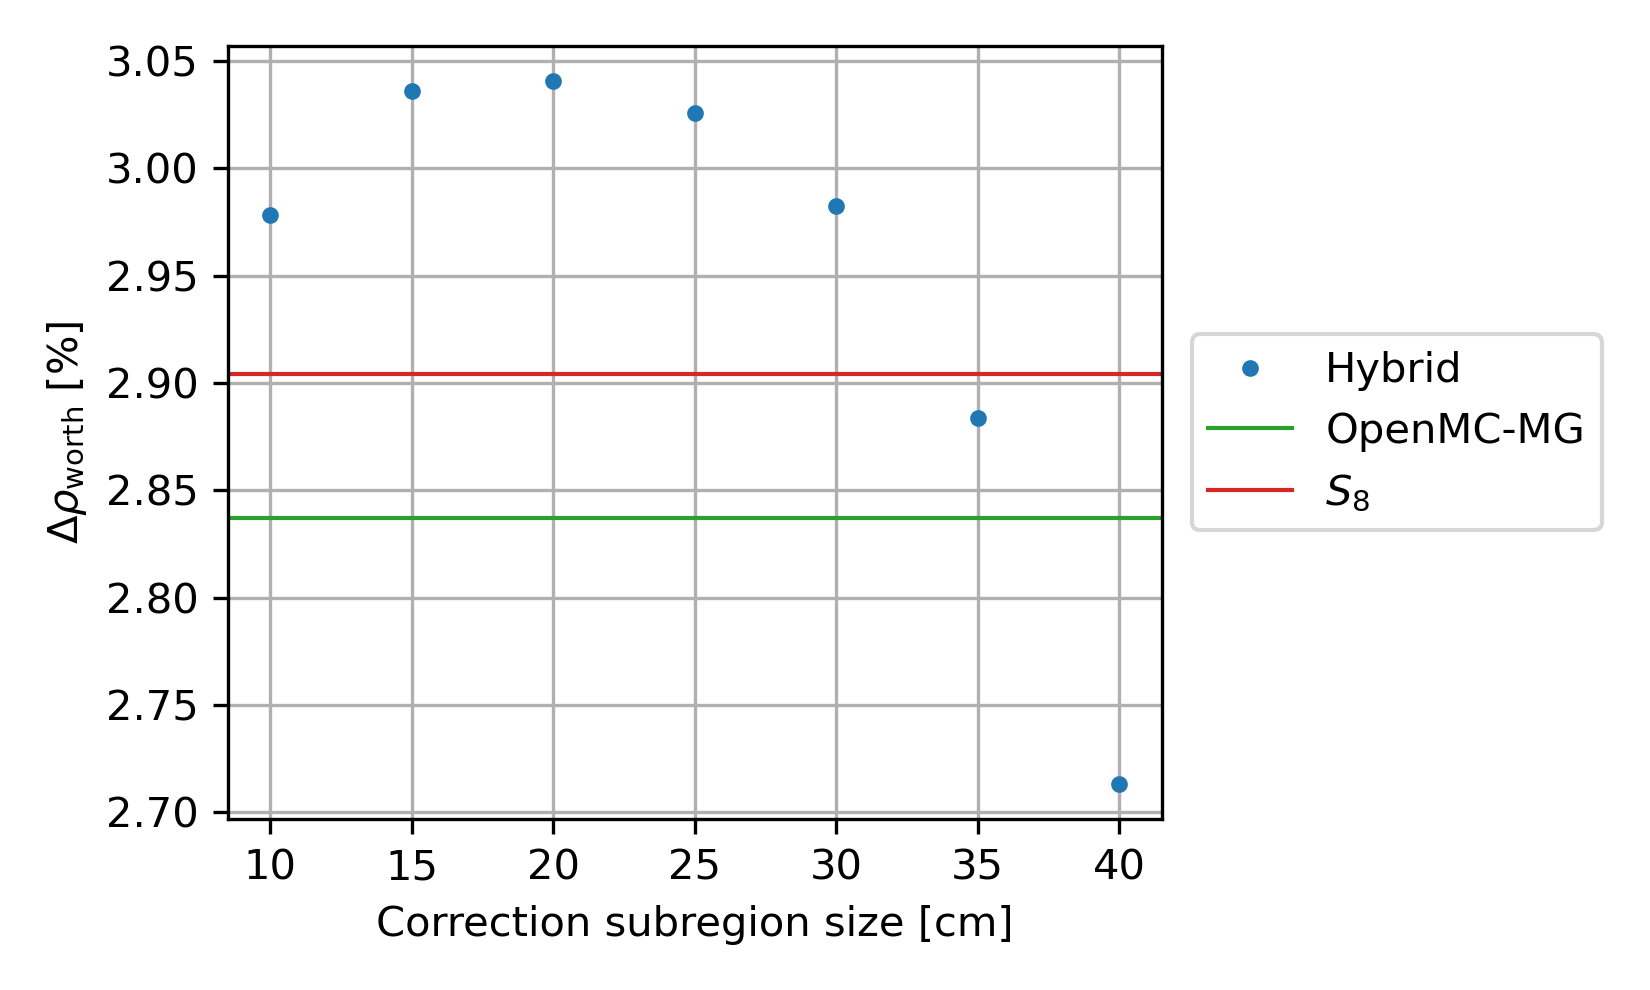
\includegraphics[width=0.8\columnwidth]{correction-size-rho}
  \caption{Percentage difference in rod worth from the hybrid method relative to OpenMC-CE for
    Cases 3a and 3b with different correction subregion sizes. The horizontal lines indicate
    equivalent rod worth differences from the OpenMC-MG and $S_8$ methods.}
  \label{fig:v1-size-rho}
\end{figure}

The $k_\text{eff}$ and rod worth results show the hybrid method is able to accurately
reproduce rod worth estimates as long as the correction subregion size remains consistent. The
correction subregion size must also be sufficiently large to capture the highly neutron-absorptive
rod's influence on the neutron flux around the rod at $x=0$ cm. The drift correction parameter
distributions in Figure \ref{fig:3b-drift} indicate that the influence of the rod on the drift, and
consequently the flux, extend to approximately $x=5$ cm before the drift distribution settles on a
regular repeating pattern influenced by the fuel-graphite lattice structure. I applied a consistent
correction subregion size of 10 cm for Cases 2 and 3 since it sufficiently meets the requirements
discussed while also minimizing the computational cost of the $S_8$ subsolver. Other reactor
designs consisting of different material components may require different minimum correction
subregion sizes.

\subsubsection{Relaxing the $S_N$ subsolver convergence threshold}

As described in Section \ref{sec:hybrid-algorithm}, the hybrid $S_N$-diffusion method works by
iteratively coupling a neutron diffusion solver and a $S_N$ subsolver with the latter generating
drift correction parameters for the former. Excluding the initial neutron diffusion calculation,
each outer (fixed point) iteration comprises of an inner $S_N$ calculation on the correction
subregion and an inner neutron diffusion calculation on the entire domain. The \gls{FEM} algorithm
in Moltres determines an individual solver reaches convergence when the combined
residual contributions fall below a specified convergence tolerance threshold. The fixed point
iteration scheme under the \texttt{MultiApps} system in Moltres for coupling multiple individual
solvers (referred to as apps) requires users to specify a main app for the final convergence check
after each outer iteration to terminate the iterations. The scheme also requires users to set a
fixed point convergence tolerance value independent of the tolerance values of each individual
solver. Naturally, the fixed point tolerance value must be equal to or greater than the tolerance
value of the main individual solver for the possibility of overall convergence. The hybrid method
implementation in Moltres sets the neutron diffusion solver as the main app and the $S_N$ subsolver
as the sub app.

The hybrid method shares some similarities with diffusion-based \gls{HOLO} acceleration schemes
(refer to Section \ref{sec:drift-correction}) for the neutron transport methods which do not
require the neutron transport side of the calculations to fully converge
\cite{reynolds_analysis_2023, wang_diffusion_2014}.
The typical convergence threshold value required for converged neutron flux calculations in Moltres
is $10^{-8}$; I set the convergence tolerance value to $10^{-8}$ for the neutron diffusion solver
and the fixed point scheme. I varied the convergence tolerance value for the $S_N$ subsolver to 
find the optimal value for maintaining sufficient solution accuracy and minimizing computational
costs; tightening the $S_N$ convergence tolerance value generally results in more outer iterations
performed before the solver meets the fixed point convergence tolerance.
Table \ref{table:sn-tol} lists the number of outer iterations required by the hybrid method for
a given set of $S_8$ subsolver convergence tolerance values in Case 3b.

\begin{table}[htb]
  \centering
  \caption{Number of outer iterations in hybrid method calculations of Case 3b for a given set of
  convergence tolerance values imposed on the $S_8$ subsolver.}
  \begin{tabular}{l S S S S S S}
    \toprule
    $S_8$ subsolver tolerance, $\epsilon_\text{tol}$ & {$10^{-8}$} & {$10^{-7}$} & {$10^{-6}$} & {$10^{-5}$} & {$10^{-4}$} & {$10^{-3}$} \\
    \midrule
    Number of outer iterations & 3 & 3 & 3 & 2 & 2 & 1 \\
    \bottomrule
  \end{tabular}
  \label{table:sn-tol}
\end{table}

Figure \ref{fig:sn-tol} shows the $k_\text{eff}$ error estimates relative to the reference value
when $\epsilon_\text{tol}=10^{-8}$. The hybrid method exhibits superlinear convergence ($q=1.333$)
with respect to the $S_N$ subsolver convergence tolerance value. Based on the results, setting
$\epsilon_\text{tol}$ to $10^{-5}$ is the best balance between accuracy and computational
cost because the $k_\text{eff}$ error is less than 0.01 pcm and the number of outer iterations
would increase from 2 to 3 if the tolerance value is further tightened.

\begin{figure}[htb!]
  \centering
  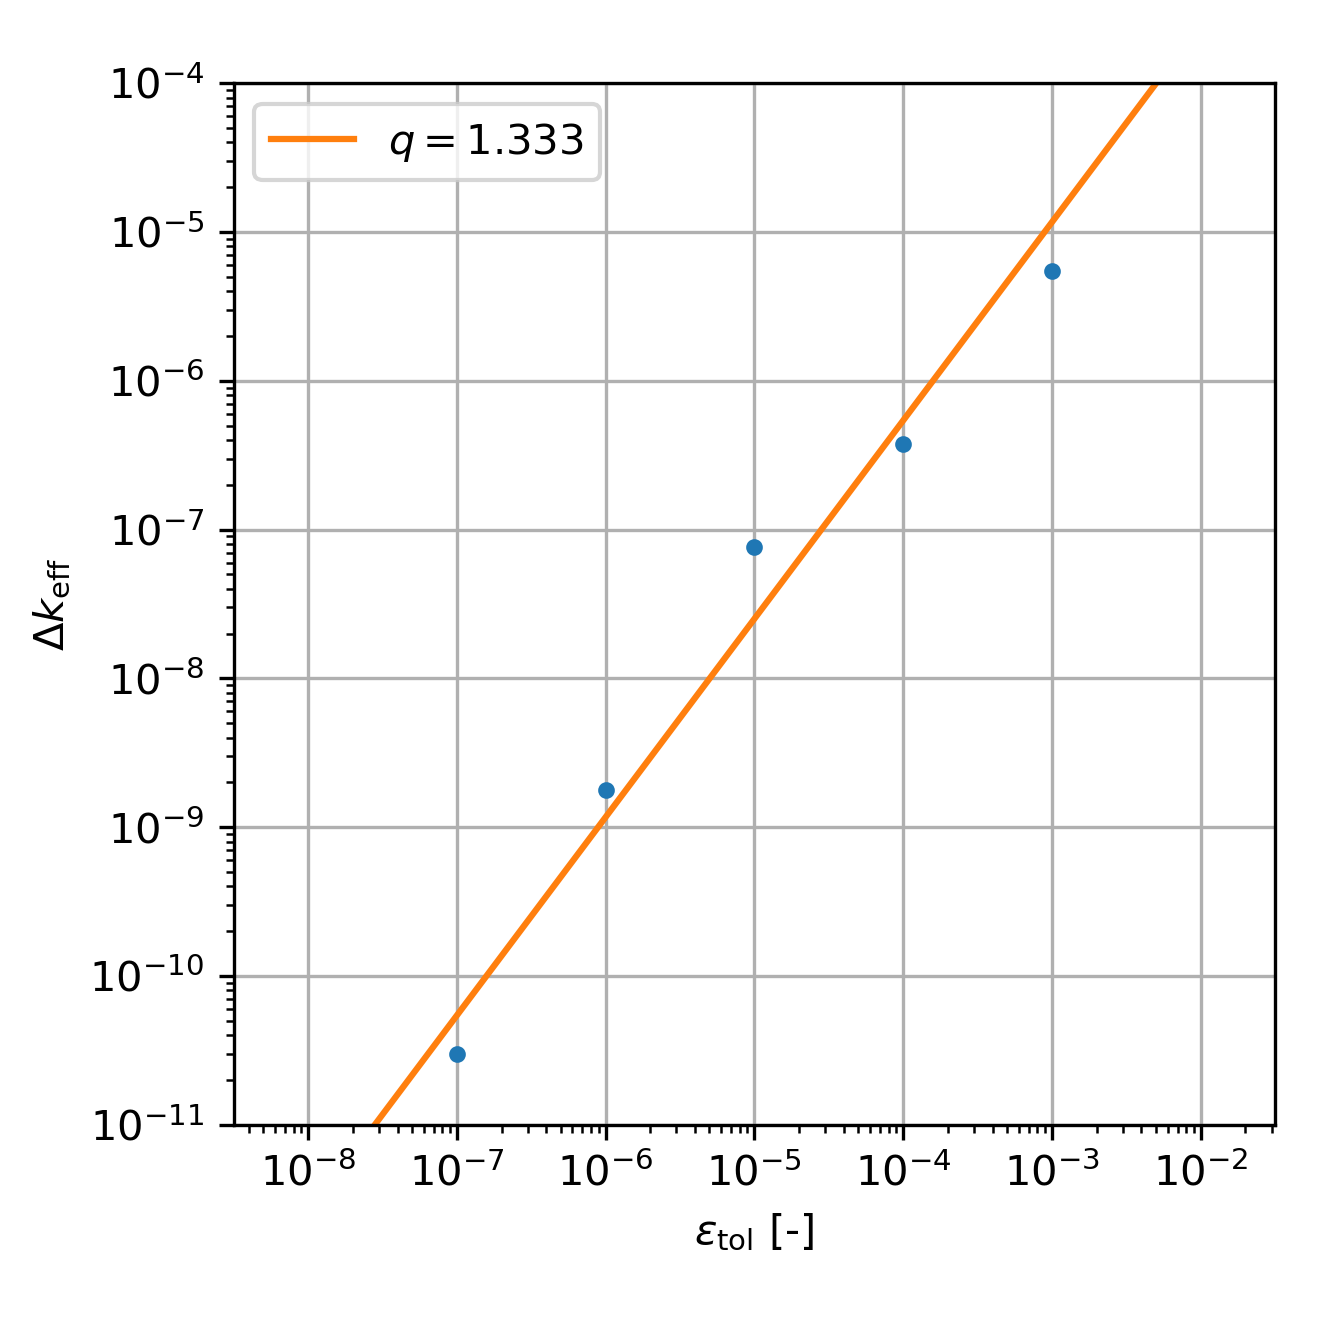
\includegraphics[width=0.6\columnwidth]{sn-tol}
  \caption{$k_\text{eff}$ error estimates of Case 3b for a range of convergence tolerance values
  imposed on the $S_8$ subsolver relative to the reference $k_\text{eff}$ value when
  $\epsilon_\text{tol}=10^{-8}$. The $q=1.333$ line represents the approximate rate of
  convergence.}
  \label{fig:sn-tol}
\end{figure}

\section{2-D Neutronics Models \& Results} \label{sec:2d-results}

\subsection{2-D Neutronics Model Setup} \label{sec:2d-model-setup}

Figures \ref{fig:1/4-geom} and \ref{fig:full-geom} show the 2-D quarter-core and full-core
\gls{MSRE} models investigated. I adapted the models from the horizontal cross section of the
\gls{MSRE} numerical benchmark model \cite{fratoni_molten_2020} with the
following differences in the 2-D \gls{MSRE} model for this work:

\begin{itemize}
  \item Ignored thermal expansion of all reactor components.
  \item Modeled the control rods as perfectly annular cylinders instead of beaded control elements
    strung on flexible steel cables. Ignored the inconel shells encasing the control elements and
    the steel helical cables linking the control elements together.
  \item Set channel pitch, width, and length to 2, 0.2, and 1.2 inches, respectively.
  \item Homogenized the INOR-8, graphite, and molten salt regions in the sample basket.
  \item Modified the outer edge of the core graphite to be circular with no jagged edges.
  \item Replaced partial channels with full-size channels near the edge of the core graphite.
  \item Ignored the thermal insulation and shield structures outside the core.
\end{itemize}

The differences listed above, along with other changes in the 3-D model, result in negligible
changes to the $k_\text{eff}$ (refer to Section 5.6) relative to the \gls{MSRE} benchmark model
\cite{fratoni_molten_2020}.

\begin{figure}[htb!]
  \centering
  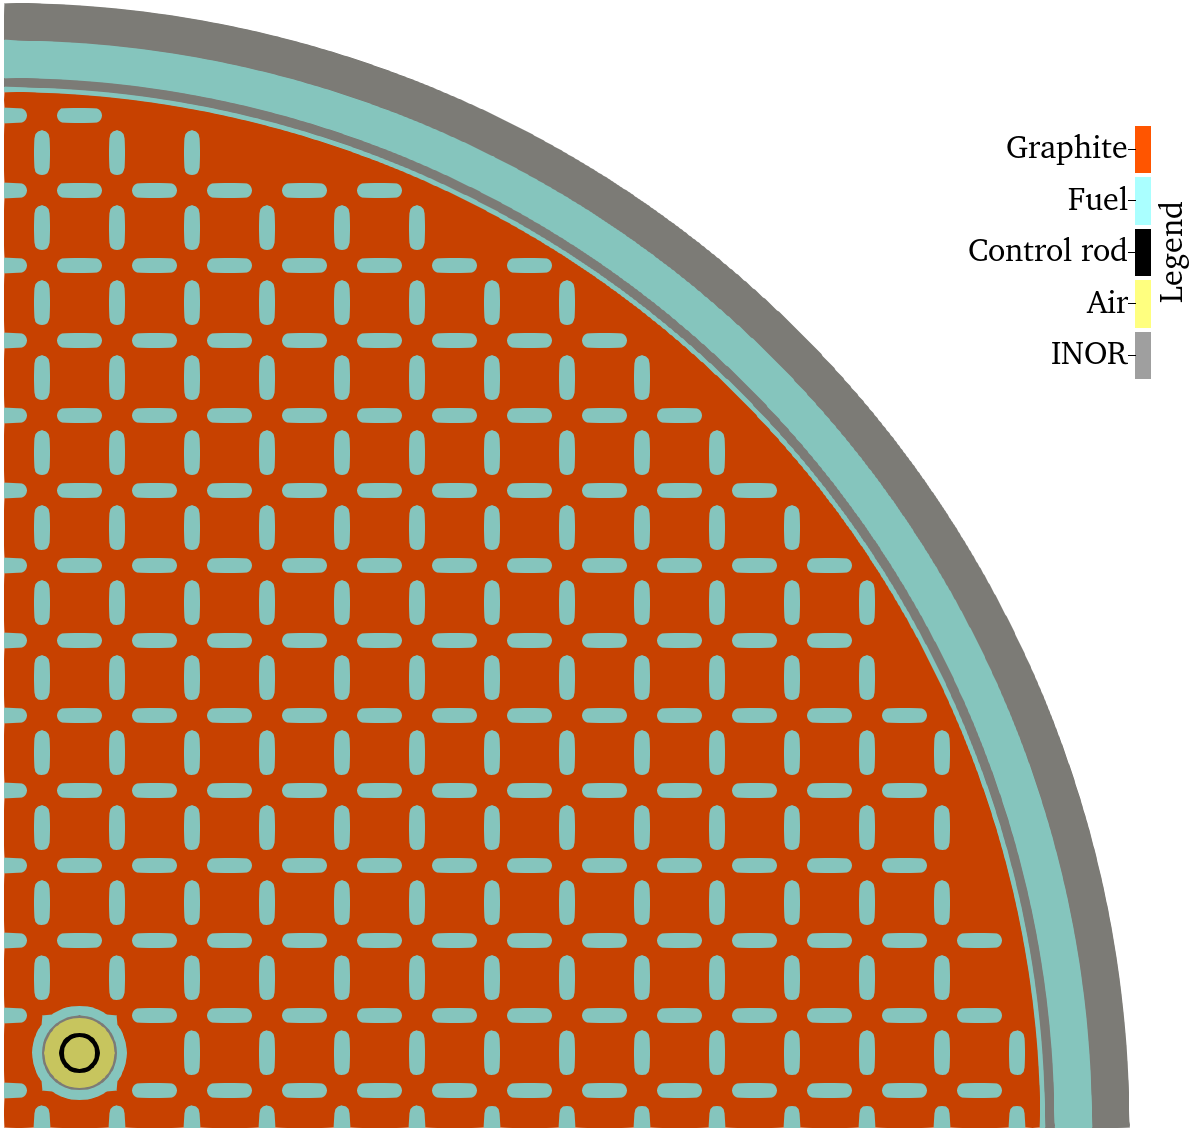
\includegraphics[width=\columnwidth]{quarter-core-geom}
  \caption{2-D \gls{MSRE} quarter-core model based on the horizontal cross section of the actual
  \gls{MSRE} geometry.}
  \label{fig:1/4-geom}
\end{figure}

\begin{figure}[htb!]
  \centering
  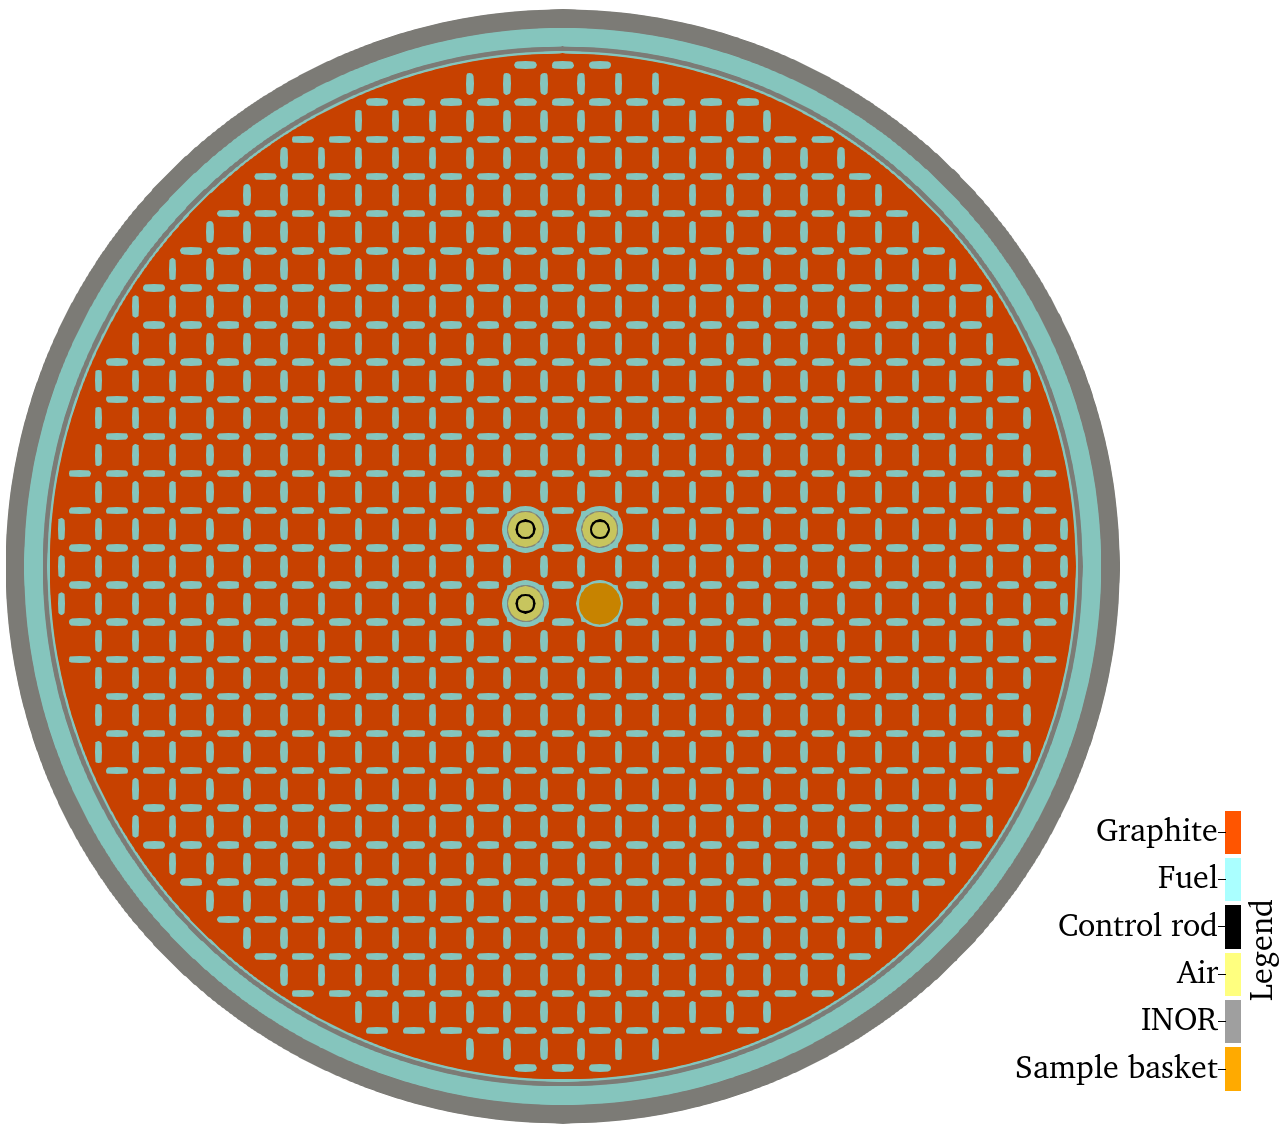
\includegraphics[width=\columnwidth]{full-core-geom}
  \caption{2-D \gls{MSRE} full-core model based on the horizontal cross section of the actual
  \gls{MSRE} geometry.}
  \label{fig:full-geom}
\end{figure}

\begin{table}[htb]
  \small
  \centering
  \setlength\tabcolsep{4pt}
  \caption{\gls{MSRE} molten salt composition when the $^{235}$U loading was at 65.25 kg.}
  \begin{tabular}{l S S S S S S S}
    \toprule
    Element & {Li} & {Be} & {Zr} & {Hf} & {$^{234}$U} & {$^{235}$U} & {$^{236}$U} \\
    \midrule
    Composition [kg] & 507.27 & 293.96 & 513.97 & 0.0029 & 0.67 & 65.25 & 0.27 \\
    \bottomrule
  \end{tabular}
  \begin{tabular}{l S S S S S S}
    \toprule
    Element & {$^{238}$U} & {Fe} & {Cr} & {Ni} & {O} & {F} \\
    \midrule
    Composition [kg] & 141.91 & 0.75 & 0.13 & 0.14 & 2.27 & 3103.22 \\
    \bottomrule
  \end{tabular}
  \label{table:2d-salt-composition}
\end{table}

INOR-8, also referred to as Hastelloy N, is a nickel-based alloy used for structural components in
the \gls{MSRE} \cite{robertson_msre_1965}.
Table \ref{table:2d-salt-composition} lists the molten salt composition for the 2-D models. The
$^{235}$U loading of 65.25 kg is the amount at which the \gls{MSRE} first achieved criticality. The
control rods consist of the original \gls{MSRE} 70 wt\% Gd$_2$O$_3$-30 wt\% Al$_2$O$_3$ mixture.
The models impose neutron vacuum boundary conditions on the outermost boundary of the INOR-8
vessel structure. The quarter-core model imposes neutron reflecting boundary conditions along the
left and bottom straight edges (Figure \ref{fig:1/4-geom}). Note that the quarter-core and
full-core models are not identical because the full-core model contains a sample basket instead of
a control rod in the lower-right segment of Figure \ref{fig:full-geom-closeup}.

\begin{figure}[htb!]
  \centering
  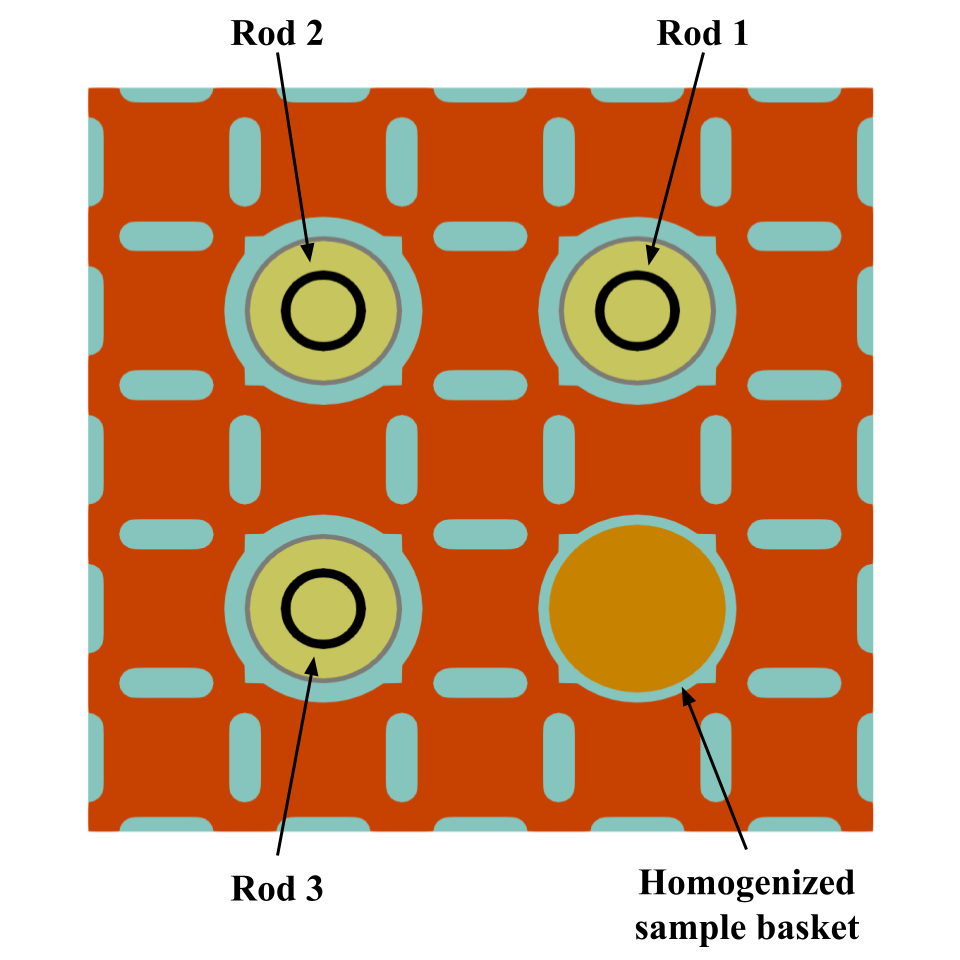
\includegraphics[width=0.7\columnwidth]{full-core-closeup}
  \caption{Detailed view of the control rod thimbles and sample basket in 2-D \gls{MSRE} full-core
    model.}
  \label{fig:full-geom-closeup}
\end{figure}

I ran neutronics simulations on the quarter- and full-core models on OpenMC under both continuous
energy (OpenMC-CE) and multigroup (OpenMC-MG) modes, and on Moltres with the hybrid $S_N$-diffusion
and neutron diffusion methods. The hybrid method ran with the $S_8$ angular discretization scheme
and up to 2nd-order scattering approximations for the $S_N$ subsolver. I simulated the
quarter-core model with and without the control rod in the air-filled rod thimble; air replaces the
control rod material when the rod is removed. For the full-core model, I considered four rod
configurations: no rods present, rod 1 present, rods 1 \& 2 present, and rods 1, 2 \& present.
Other than providing a close-up view of the core center, Figure \ref{fig:full-geom-closeup} also
presents the correction subregion on which the $S_8$ subsolver of the hybrid method generates
drift correction parameters for the coupled diffusion solver.

\FloatBarrier

\subsection{2-D Neutronics Numerical Results \& Discussion} \label{sec:2d-nts-results}

\subsubsection{2-D Quarter-Core}

Table \ref{table:quarter-core} details the $k_\text{eff}$ and control rod worth estimates and error
values relative to OpenMC-CE. For the ``No Rod'' case, OpenMC-CE estimated the $k_\text{eff}$ to be
1.11209(43). The OpenMC-MG, hybrid, and neutron diffusion methods performed
similarly to one another with reactivity errors ranging from 618 pcm to 773 pcm relative to
OpenMC-CE. Based on $k_\text{eff}$ alone, the hybrid method performed marginally worse than the
neutron diffusion method. However, for the ``Rod'' case, then neutron diffusion method saw a
change in sign of the error to -816 pcm. The errors for OpenMC-MG and the hybrid method
remained positive and reduced to 446 pcm and 760 pcm, respectively. Consequently, when taking the
difference in reactivities to estimate the rod worth, the neutron diffusion method performed
significantly worse than OpenMC-MG and the hybrid method. OpenMC-CE estimated the rod worth to be
8370(53) pcm. The neutron diffusion method overestimated the rod worth by 1484 pcm. The hybrid
method improved significantly on the neutron diffusion method with a rod worth estimate that is
only 13 pcm
higher than OpenMC-CE. OpenMC-MG reported a larger error of 172 pcm likely due to favorable error
cancellation with the hybrid method and statistical uncertainties with the Monte Carlo methods.
The OpenMC-CE and OpenMC-MG rod worth estimates agree within two standard deviations of each other.

\begin{table}[htb]
  \small
  \centering
  \caption{$k_\text{eff}$ and control rod worth estimates for the 2-D quarter-core \gls{MSRE}
    model. Error values are relative to OpenMC-CE.}
  \begin{tabular}{l S[table-format=1.5(2)] S S[table-format=1.5(2)] S S[table-format=4(2)] S}
    \toprule
    \multirow{2}{*}{Method} & \multicolumn{2}{c}{No Rod} & \multicolumn{2}{c}{Rod} & \multicolumn{2}{c}{Rod worth} \\
                            & {$k_\text{eff}$} & {Error [pcm]} & {$k_\text{eff}$} & {Error [pcm]} & {$\Delta\rho_\text{worth}$ [pcm]} & {Error [pcm]} \\
                            \cmidrule(r){1-1} \cmidrule(rl){2-3} \cmidrule(rl){4-5} \cmidrule(l){6-7}
	  OpenMC-CE & 1.11209(43) & {-} & 1.01740(42) & {-} & 8370(53) & {-} \\
	  OpenMC-MG & 1.11979(42) & 618 & 1.02204(41) & 446 & 8541(51) & 172 \\
      Diffusion & 1.12059 & 682 & 1.00903 & -816 & 9867 & 1484 \\
      Hybrid & 1.12174 & 773 & 1.02532 & 760 & 8383 & 13 \\
    \bottomrule
  \end{tabular}
  \label{table:quarter-core}
\end{table}

\begin{figure}[htb!]
  \centering
  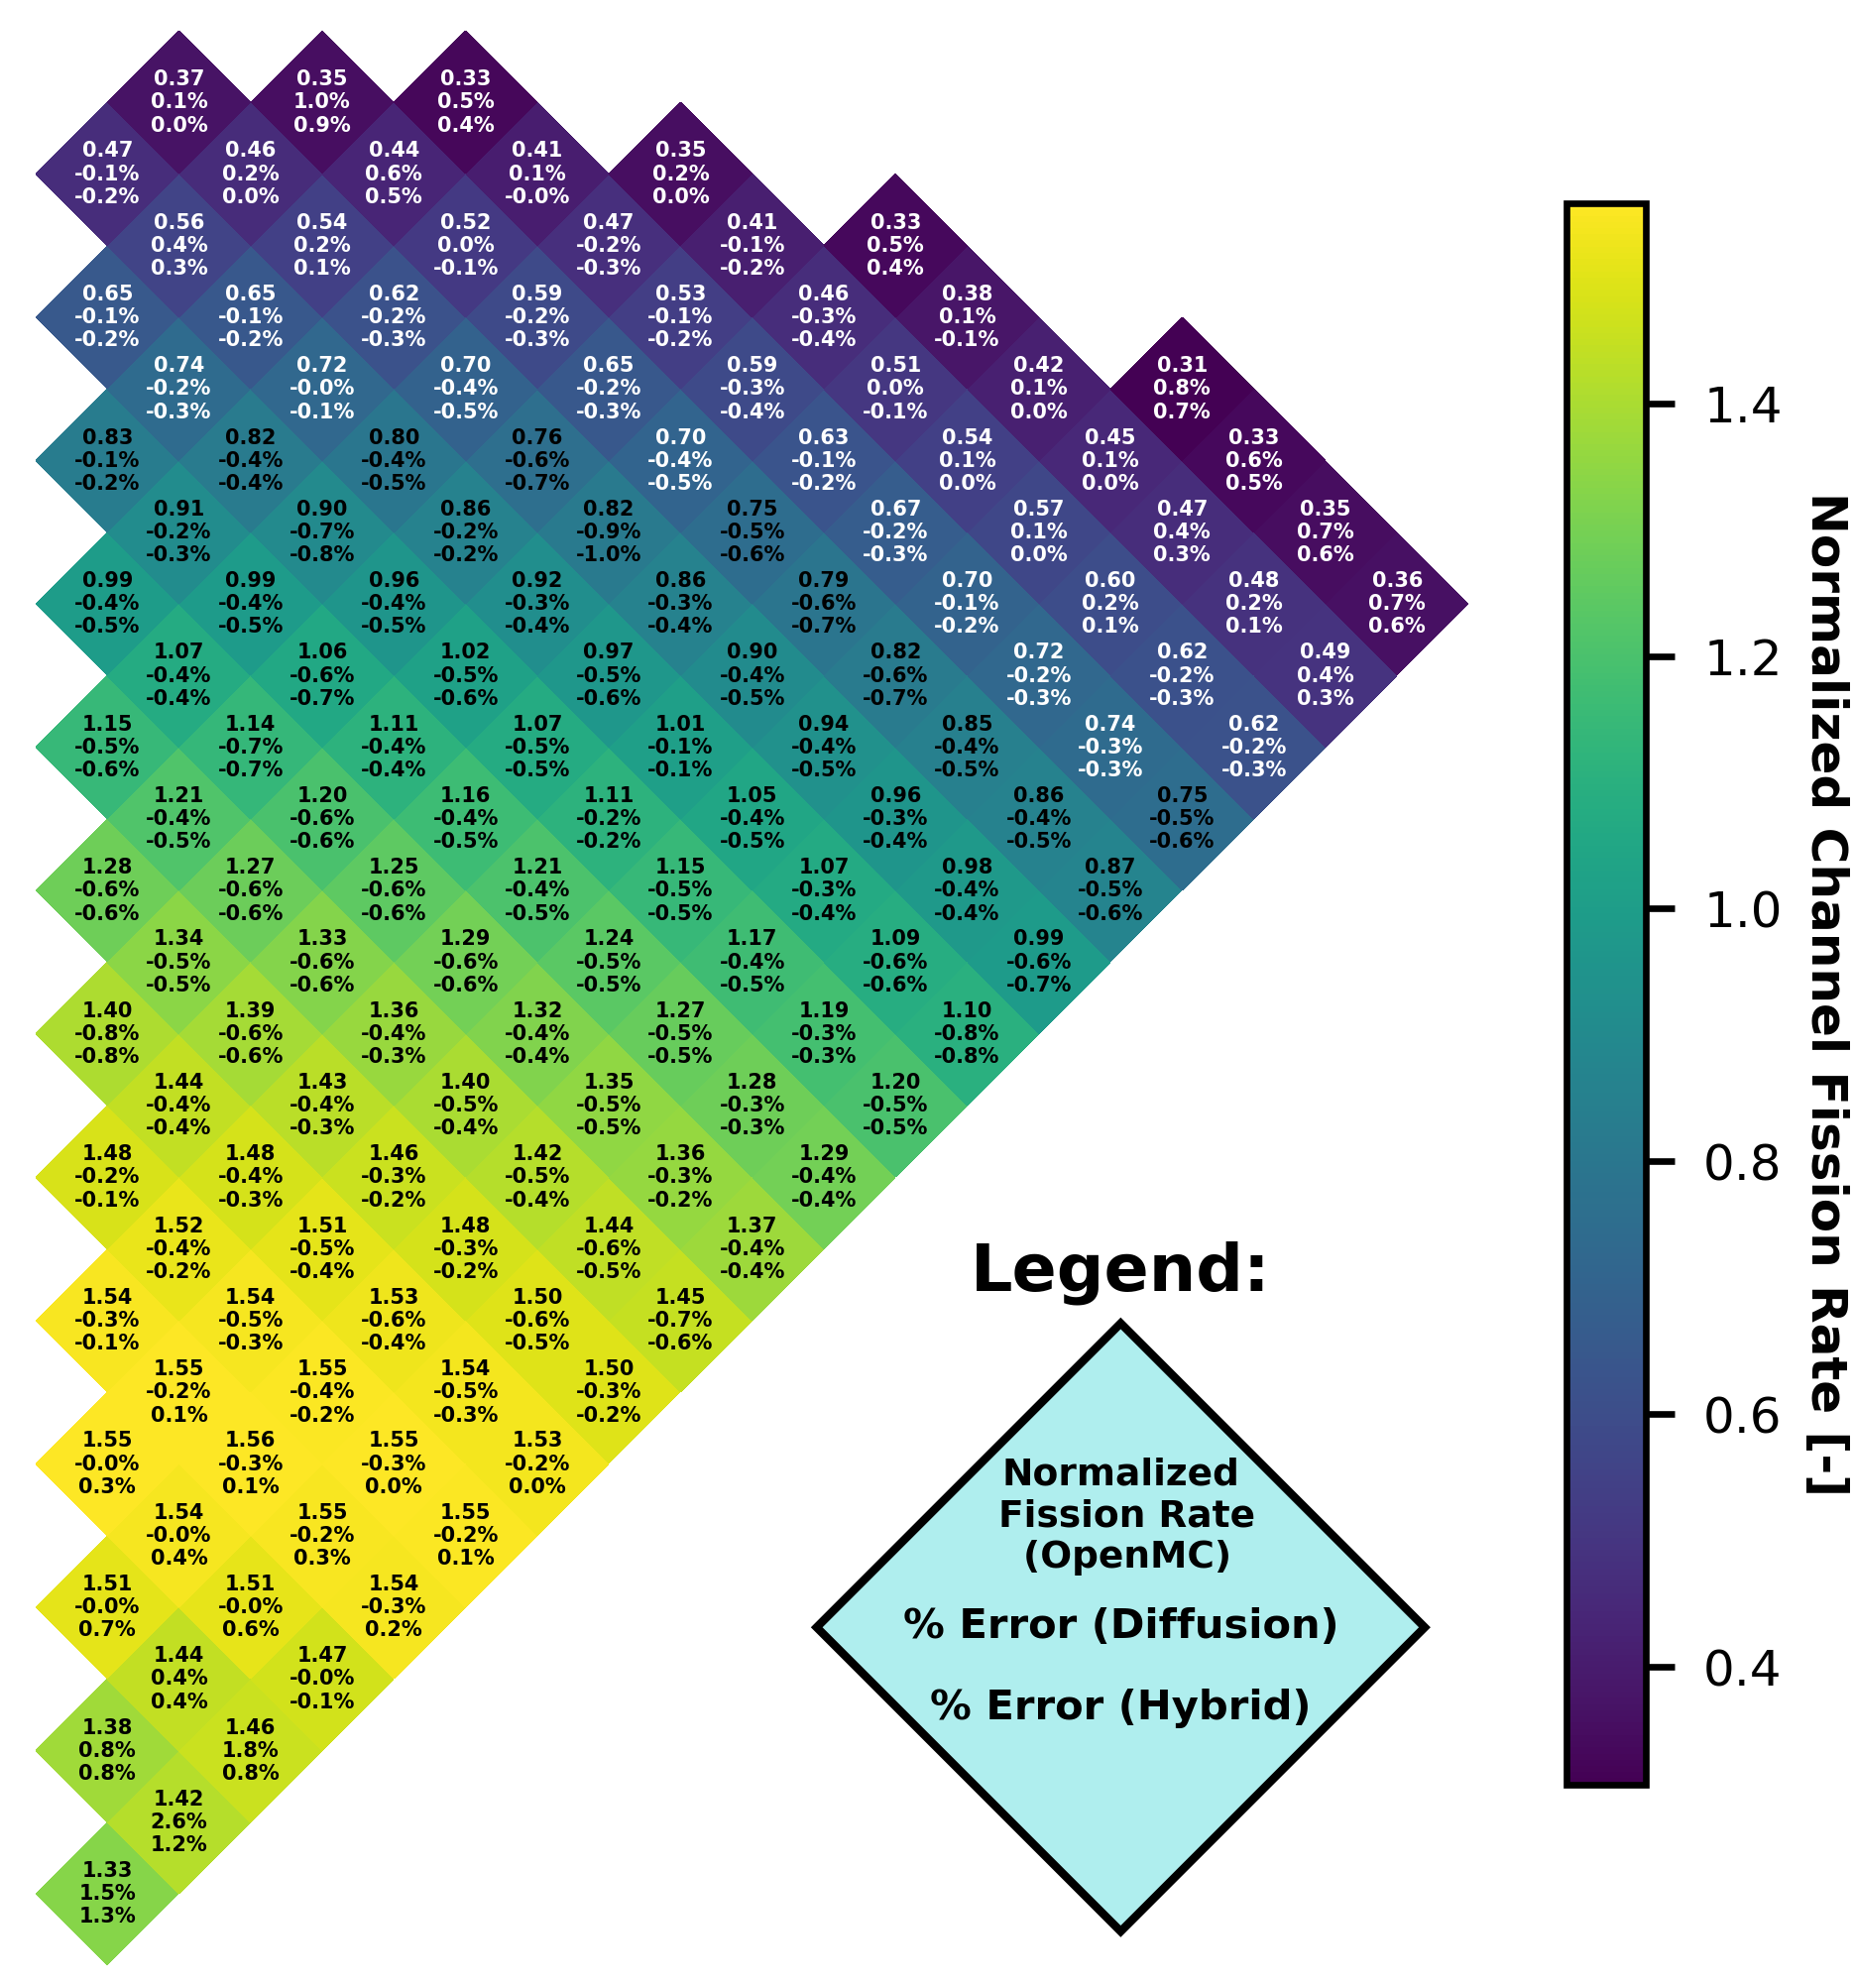
\includegraphics[width=\columnwidth]{msre-quarter-no-rod-power}
  \caption{Normalized channel fission rate distribution of the 2-D \gls{MSRE} quarter-core model.
  This figure depicts the 1/8th-core distribution due to symmetry about the diagonal.}
  \label{fig:1/4-no-rod}
\end{figure}

\begin{figure}[htb!]
  \centering
  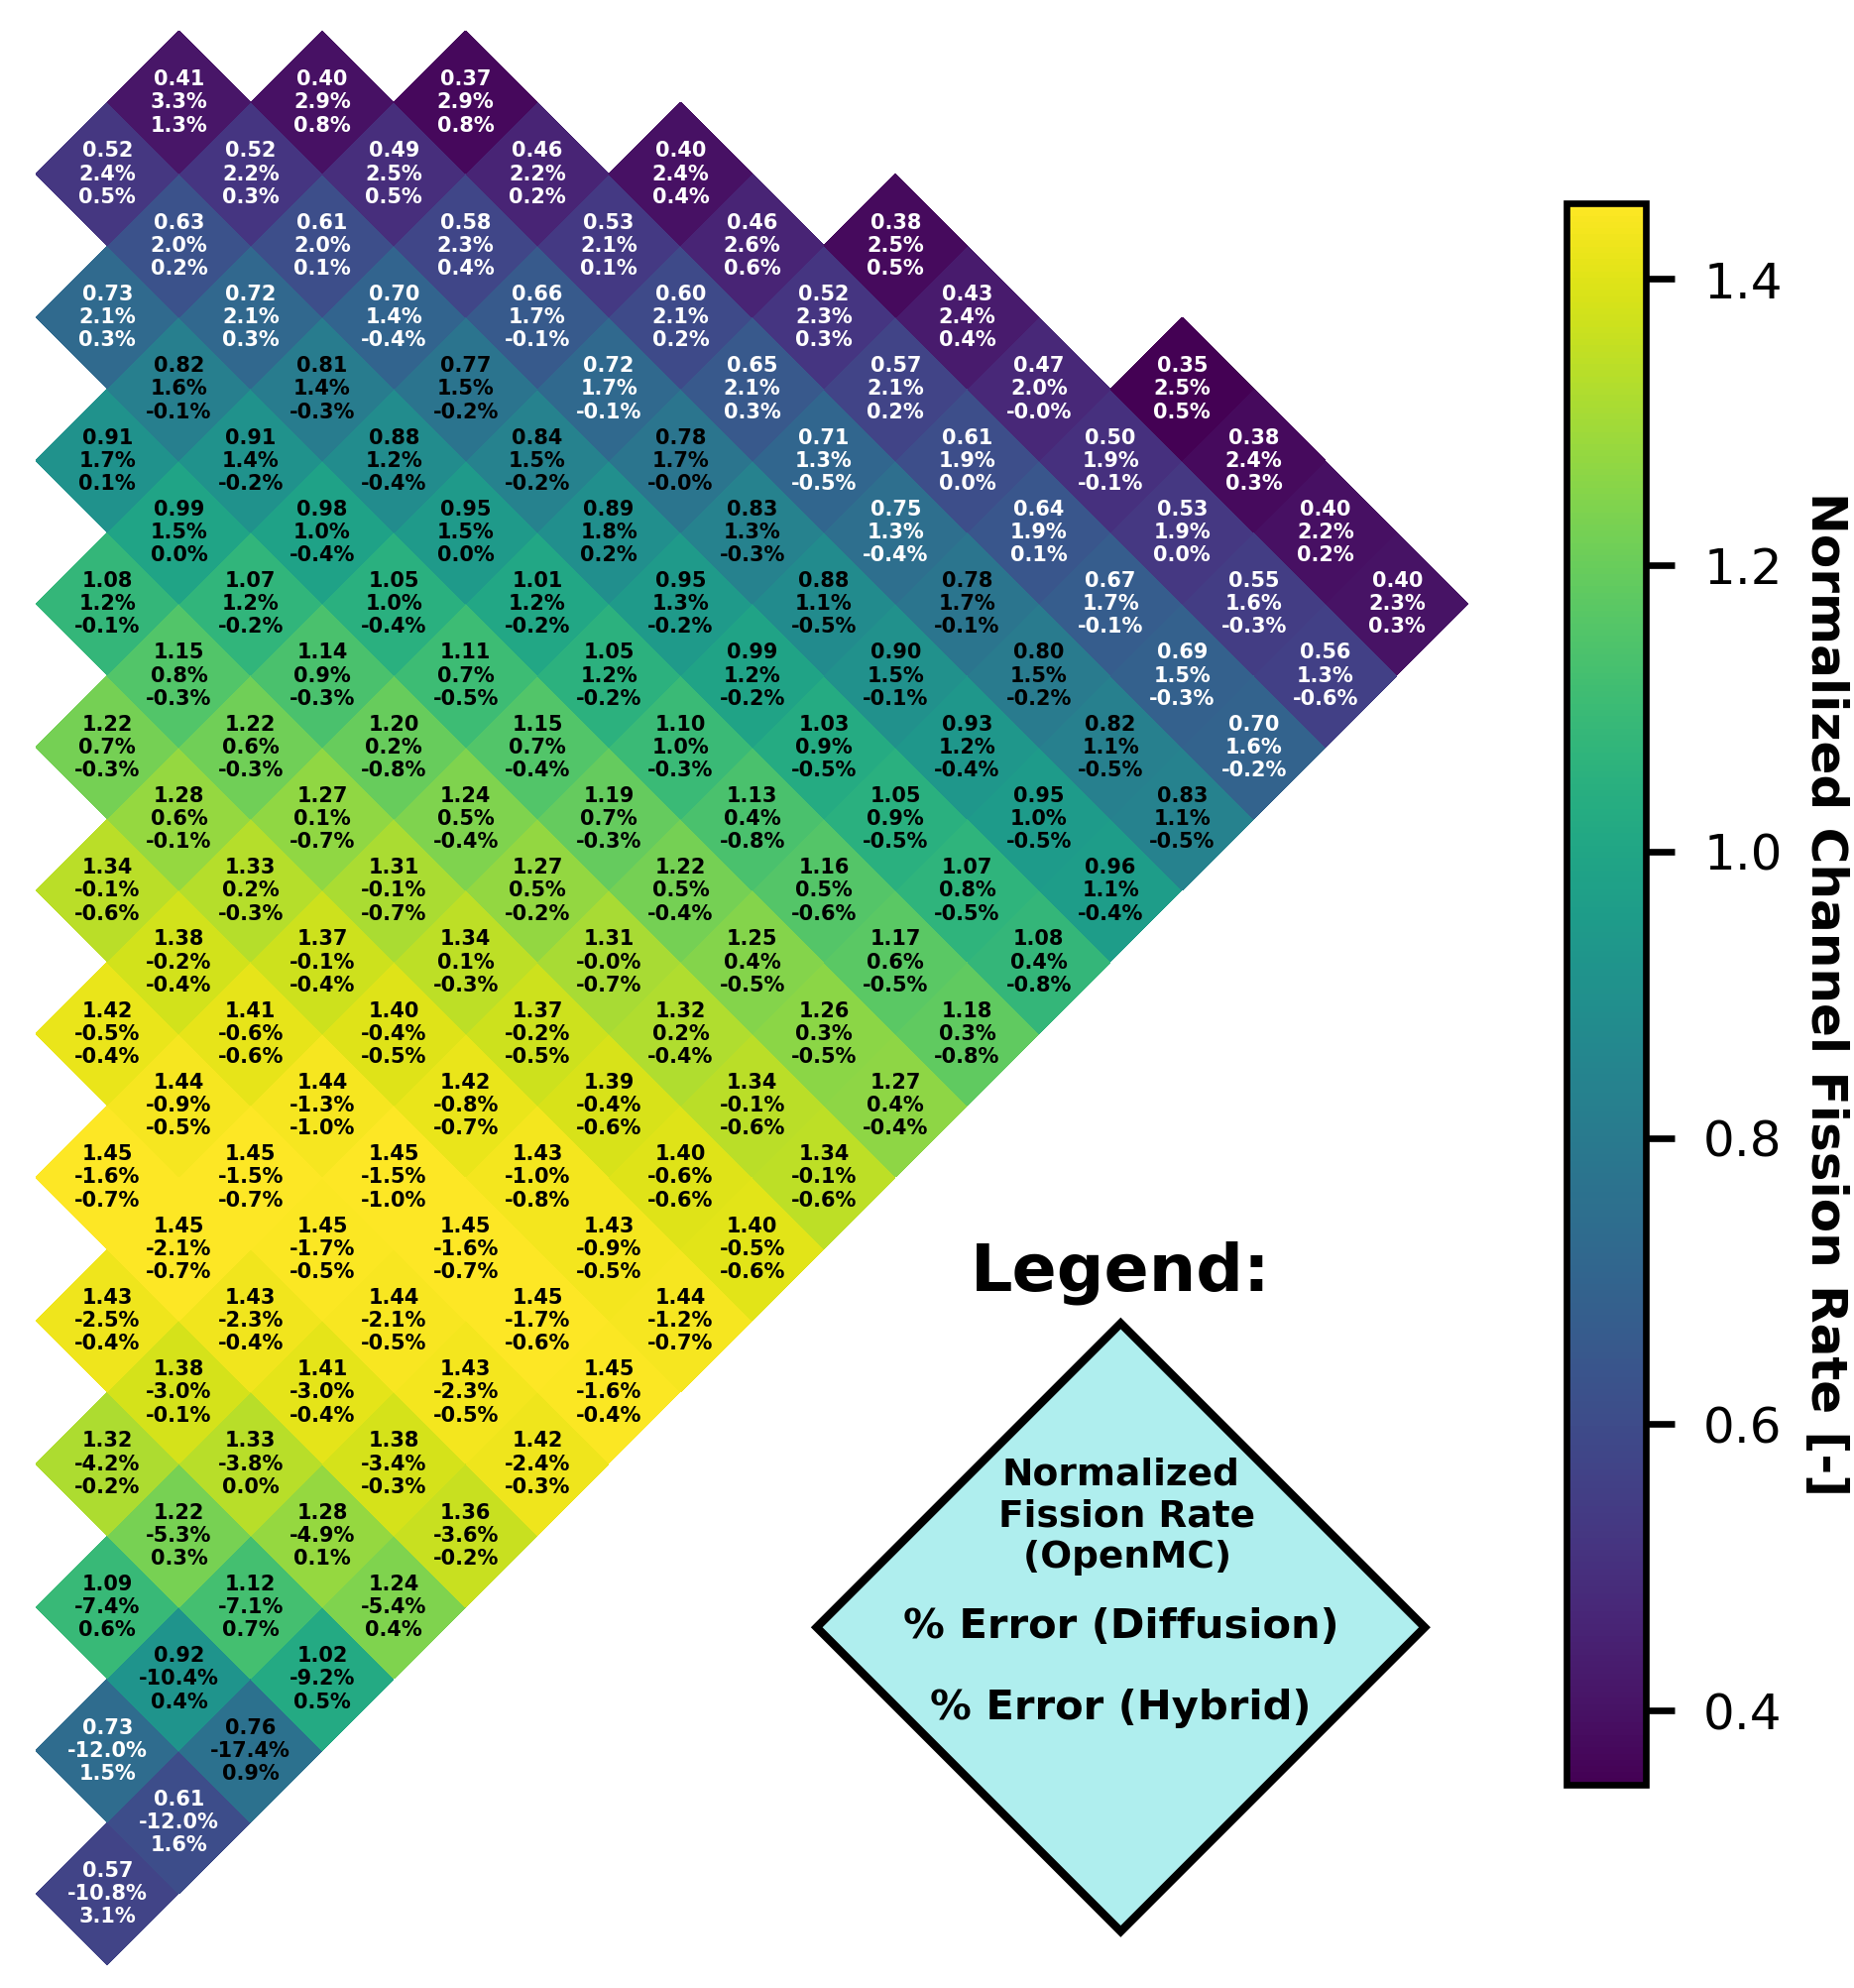
\includegraphics[width=\columnwidth]{msre-quarter-rod-power}
  \caption{Normalized channel fission rate distribution of the 2-D \gls{MSRE} quarter-core model.
  This figure depicts the 1/8th-core distribution due to symmetry about the diagonal.}
  \label{fig:1/4-rod}
\end{figure}

\FloatBarrier

I also calculated the normalized channel fission rate distribution by integrating the fission rate
within each fuel salt channel and normalizing the values such that the integrated fission rate in
each channel averages to 1 as follows
%
\begin{align}
  \text{Normalized fission rate of channel }i &= \frac{\text{Fission rate in channel }i}{
  \text{Total fission rate}}\cdot\frac{\text{Total number of channels}}{
    \text{Total fission rate in channels}} \nonumber \\
                                              &= \frac{\sum^G_{g=1}\int_{V_i}\Sigma_{f,g}
  \phi_g(\vec{r})}{\sum^G_{g=1}\int_V\Sigma_{f,g}\phi_g(\vec{r})}\cdot\frac{N_i}{
  \sum^{N_i}_{i=1}\sum^G_{g=1}\int_{V_i}\Sigma_{f,g}\phi_g(\vec{r})}.
\end{align}
%
The total fission rate includes fission rate contributions from peripheral fuel salt regions.
Figures \ref{fig:1/4-no-rod} and \ref{fig:1/4-rod} show the normalized fission rate distributions
of the quarter-core model for the ``No Rod'' and ``Rod'' cases, respectively. I presented 1/8th
slices of the core in the figures because the distributions are symmetrical about the $y=x$ line
outside of statistical variances for OpenMC-CE. I combined the midpoints between the centroids of
neighboring fuel salt channels to form the diamond lattices shown in the figures.
Each diamond element in the figures corresponds a horizontally or vertically oriented channel
depicted in Figure \ref{fig:1/4-geom}. The lattice also provides a guide for subdividing the
annular fuel regions around the control rod thimbles. The fission rate
distributions omit four channels along the outer edge due to the proximity to peripheral annular
fuel regions and the consequent difficulty in accurately tallying fission rates.

In the ``No Rod'' case, the peak channel fission rate occured several channels away from the
physical center of the reactor core. The presence of the empty (air-filled) rod thimble depressed
fission rates near the center. The neutron diffusion and hybrid methods report similar percentage
errors relative to OpenMC-CE except near the center. While the hybrid method benefits from drift
corrections, the neutron diffusion method's reliance on scalar diffusion coefficients tends to
artificially flatten neutron fluxes in near-void regions. Therefore, the largest percentage errors
from the neutron diffusion method occurred in the second and third diamond elements
diagonally up from the bottom which represent the annular fuel region surrounding the rod thimble.
In the ``Rod'' case, the introduction of the control rod shifted the peak further away from the
center as expected of a highly neutron-absorbing material. The rod further worsened fission rate
errors for the neutron diffusion method with large errors of 1\% or more at the core center and
periphery. On the other hand, the fission rate errors for the hybrid method largely remained below
1\%.

\begin{table}[htb]
  \small
  \centering
  \caption{Absolute mean and maximum percentage errors in the normalized channel fission rates of
  the 2-D \gls{MSRE} quarter-core models relative to OpenMC. The mean relative standard deviation of
  OpenMC normalized channel fission rates is 0.20\%.}
  \begin{tabular}{l S S S S}
    \toprule
    \multirow{2}{*}{Method} & \multicolumn{2}{c}{No Rod} & \multicolumn{2}{c}{Rod} \\
                            & {Mean [\%]} & {Maximum [\%]} & {Mean [\%]} & {Maximum [\%]} \\
                            \cmidrule(r){1-1} \cmidrule(rl){2-3} \cmidrule(l){4-5}
    Diffusion & 0.40 & 2.63 & 2.01 & 17.44 \\
    Hybrid & 0.40 & 1.32 & 0.43 & 3.08 \\
    \bottomrule
  \end{tabular}
  \label{table:quarter-core-power}
\end{table}

Table \ref{table:quarter-core-power} shows the absolute mean and maximum percentage errors of the
normalized channel fission rates from the neutron diffusion and hybrid methods relative to
OpenMC-CE. Overall, the hybrid method reported smaller percentage errors than the neutron diffusion
method. The absolute maximum percentage error from the neutron diffusion method jumped to 17.44\%
as compared to the 3.08\% for the hybrid method in the ``Rod'' case. Along with the figures, these
results demonstrate the hybrid method provides improved fission rate distribution accuracy in
the existence of near-void and highly neutron-absorbing regions.

\FloatBarrier

\subsubsection{2-D Full-Core}

I performed the same $k_\text{eff}$ and fission rate distribution analyses with the 2-D full-core
model under four configurations starting from no rod inserted to all three rods inserted. The
$k_\text{eff}$ and error estimates in Table \ref{table:full-core-k} show the same trends observed
with the 2-D quarter-core model. OpenMC-MG and the hybrid method exhibit moderate but consistent
reactivity errors of approximately the 550 pcm and 800 pcm, respectively. The neutron diffusion
method reported errors ranging from 692 pcm when no rod is inserted to -470 pcm when all three rods
are inserted. Consequently, in Table \ref{table:full-core-worth}, OpenMC-MG and the hybrid method
report accurate control rod worths within 1-3 standard deviations of OpenMC-CE while the neutron
diffusion method increasingly overestimates the rod worth as more rods are inserted.

\begin{table}[htb]
  \small
  \centering
  \caption{$k_\text{eff}$ estimates for the 2-D full-core \gls{MSRE} model with the indicated rods
    inserted. Error values are relative to OpenMC-CE.}
  \setlength\tabcolsep{2pt}
  \begin{tabular}{l S[table-format=1.5(2)] S S[table-format=1.5(2)] S S[table-format=1.5(2)] S S[table-format=1.5(2)] S}
    \toprule
    \multirow{3}{*}{Method} & \multicolumn{2}{c}{No Rod} & \multicolumn{2}{c}{Rod 1} & \multicolumn{2}{c}{Rod 1 \& 2} & \multicolumn{2}{c}{Rod 1, 2 \& 3} \\
                            & {\multirow{2}{*}{$k_\text{eff}$}} & {Error} & {\multirow{2}{*}{$k_\text{eff}$}} & {Error} & {\multirow{2}{*}{$k_\text{eff}$}} & {Error} & {\multirow{2}{*}{$k_\text{eff}$}} & {Error} \\
                            & & {[pcm]} & & {[pcm]} & & {[pcm]} & & {[pcm]} \\
                            \cmidrule(r){1-1} \cmidrule(rl){2-3} \cmidrule(rl){4-5} \cmidrule(rl){6-7} \cmidrule(l){8-9}
    OpenMC-CE & 1.09859(20) & {-} & 1.06980(21) & {-} & 1.04690(18) & {-} & 1.02688(18) & {-} \\
    OpenMC-MG & 1.10637(19) & 640 & 1.07633(20) & 567 & 1.05235(20) & 495 & 1.03262(17) & 541 \\
    Diffusion & 1.10701 & 692 & 1.07120 & 122 & 1.04415 & -252 & 1.02195 & -470 \\
    Hybrid & 1.10843 & 808 & 1.07906 & 802 & 1.05553 & 781 & 1.03582 & 841 \\
    \bottomrule
  \end{tabular}
  \label{table:full-core-k}
\end{table}

\begin{table}[htb]
  \small
  \centering
  \caption{Control rod worth estimates for the 2-D full-core \gls{MSRE} with the
  indicated rods inserted. Error values are relative to OpenMC-CE.}
  \setlength\tabcolsep{5pt}
  \begin{tabular}{l S[table-format=4(2)] S S[table-format=4(2)] S S[table-format=4(2)] S}
    \toprule
    \multirow{2}{*}{Method} & \multicolumn{2}{c}{Rod 1} & \multicolumn{2}{c}{Rod 1 \& 2} & \multicolumn{2}{c}{Rod 1, 2 \& 3} \\
                            & {$\Delta\rho_\text{worth}$ [pcm]} & {Error [pcm]} & {$\Delta\rho_\text{worth}$ [pcm]} & {Error [pcm]} & {$\Delta\rho_\text{worth}$ [pcm]} & {Error [pcm]} \\
                            \cmidrule(r){1-1} \cmidrule(rl){2-3} \cmidrule(rl){4-5} \cmidrule(l){6-7}
    OpenMC-CE & 2450(25) & {-} & 4494(23) & {-} & 6357(24) & {-} \\
    OpenMC-MG & 2523(23) & 73 & 4640(24) & 146 & 6455(22) & 98 \\
    Diffusion & 3019 & 569 & 5439 & 945 & 7519 & 1162 \\
    Hybrid & 2455 & 5 & 4521 & 27 & 6323 & -34 \\
    \bottomrule
  \end{tabular}
  \label{table:full-core-worth}
\end{table}

Plots of the normalized channel fission rate distributions for all four rod configurations are
available in Appendix \ref{chap:2d-fiss-rate}. They are best viewed in digital pdf format with
magnification due to the numerous fuel salt channels and small fonts.

Table \ref{table:full-core-power} shows the absolute mean and maximum percentage errors in the
normalized channel fission rates from the neutron diffusion and hybrid methods relative to
OpenMC-CE. Both mean and maximum percentage errors from the neutron diffusion method steadily
increase with the number of rods inserted. The mean percentage error from the hybrid method remains
constant at 0.43\% while the maximum percentage error increases marginally from 1.45\% to 2.52\%
when all three rods are inserted. These results demonstrate the hybrid method remains
effective at improving control rod worth and fission rate distribution estimates in less symmetric
geometries.

\begin{table}[htb]
  \footnotesize
  \centering
  \caption{Absolute mean and maximum percentage errors in the normalized channel fission rates of
  the 2-D \gls{MSRE} full-core models relative to OpenMC. The mean relative standard deviation of
  OpenMC normalized channel fission rates is 0.27\%.}
  \setlength\tabcolsep{2.5pt}
  \begin{tabular}{l S S S S S S S S}
    \toprule
    \multirow{2}{*}{Method} & \multicolumn{2}{c}{No Rod} & \multicolumn{2}{c}{Rod 1} & \multicolumn{2}{c}{Rod 1 \& 2} & \multicolumn{2}{c}{Rod 1, 2 \& 3} \\
                            & {Mean [\%]} & {Maximum [\%]} & {Mean [\%]} & {Maximum [\%]} & {Mean [\%]} & {Maximum [\%]} & {Mean [\%]} & {Maximum [\%]} \\
                            \cmidrule(r){1-1} \cmidrule(rl){2-3} \cmidrule(rl){4-5} \cmidrule(rl){6-7} \cmidrule(l){8-9}
    Diffusion & 0.45 & 2.95 & 0.94 & 12.61 & 1.35 & 15.34 & 1.67 & 17.09 \\
    Hybrid & 0.43 & 1.45 & 0.43 & 1.82 & 0.43 & 2.26 & 0.43 & 2.52 \\
    \bottomrule
  \end{tabular}
  \label{table:full-core-power}
\end{table}

\FloatBarrier

\section{3-D Neutronics Models \& Results} \label{sec:3d-results}

\subsection{3-D Neutronics Model Setup} \label{sec:3d-model-setup}

Figure \ref{fig:msre-picture} shows the vertical cross section of the actual \gls{MSRE} vessel.
The actual design has rounded upper and lower plena to help direct salt flow through the system.
This work uses a modified 3-D numerical \gls{MSRE} model as shown by the vertical cross section
in Figure \ref{fig:msre-geom-vert}. The model excludes the toroidal flow distributor near the top
of the vessel and reshapes the plena into right cylinders. It has the same horizontal cross section
as the 2-D model (Figure \ref{fig:full-geom}) throughout most of the salt-graphite lattice. In
addition to modifications in the 2-D model listed in Section \ref{sec:2d-model-setup}, the
3-D model includes the following modifications:

\begin{itemize}
  \item Removed the toroidal flow distributor near the top of the vessel.
  \item Reshaped the upper and lower plena into right cylinders while keeping the salt volume
    constant.
  \item Flattened the conical tops of the graphite lattice blocks.
  \item Regularized the complicated graphite lattice structure at the bottom.
  \item Set a fixed outer vessel thickness of 2.54 cm.
  \item Homogenized the lower plenum by 90.8\% salt- 9.2\% INOR-8 (vessel) by volume.
  \item Removed the reactor access nozzle and the various components within it.
  \item Added a graphite block at the bottom of the control rod thimbles.
\end{itemize}

\begin{figure}[p]
  \centering
  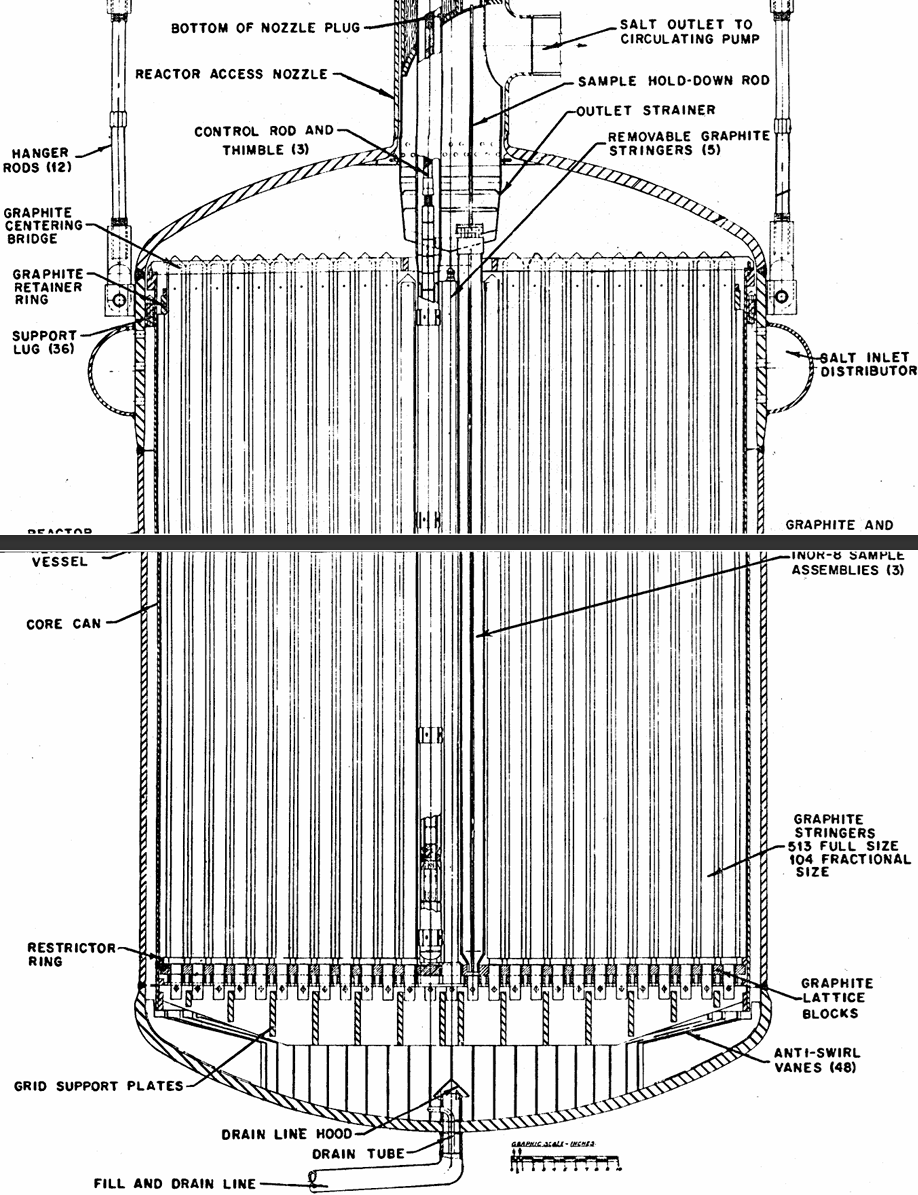
\includegraphics[width=0.97\columnwidth]{msre-picture}
  \caption{Vertical cross section of the actual \gls{MSRE} vessel. It has rounded upper and lower
  plena, and a toroidal flow distributor that distributes the salt inflow evenly as it enters the
  core through holes on the inside vessel surface of the distributor.}
  \label{fig:msre-picture}
\end{figure}

\begin{figure}[p]
  \centering
  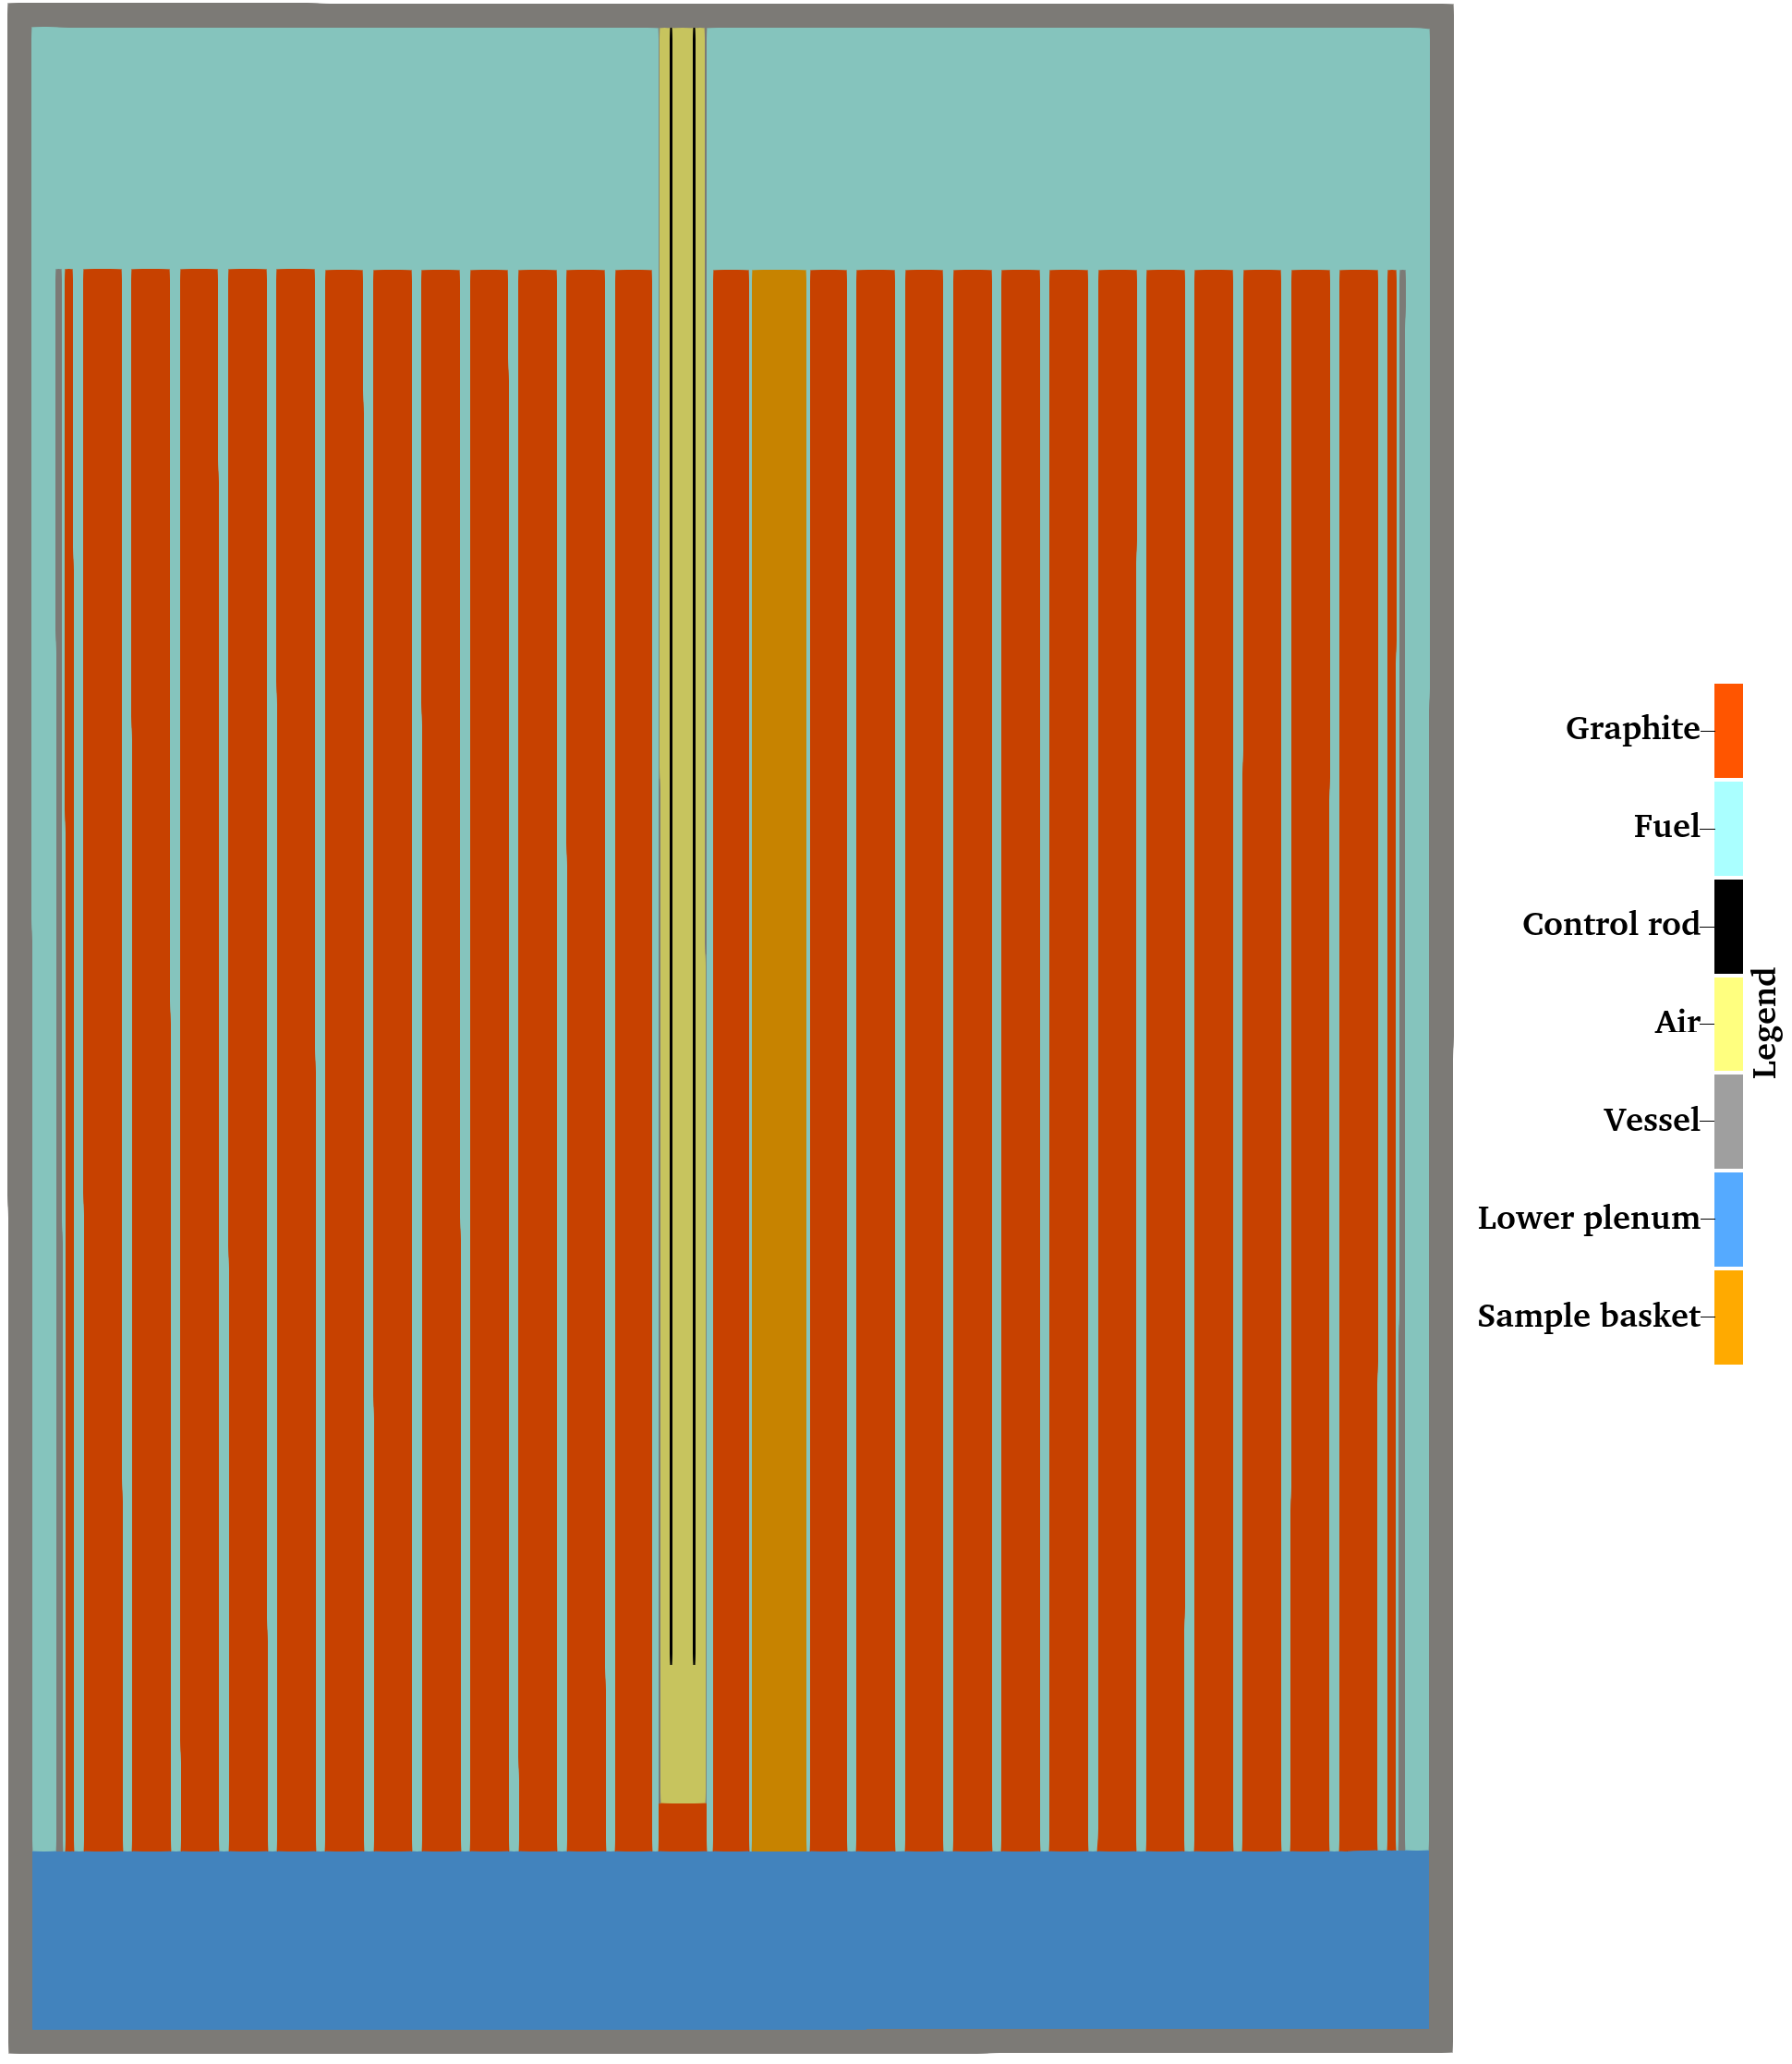
\includegraphics[width=\columnwidth]{msre-geom-vert}
  \caption{Vertical cross section of the 3-D numerical \gls{MSRE} model offset by 5.08 cm to show
  the control rod thimble and homogenized sample basket. The control rod is in its fully inserted
  position. The homogenized lower plenum consists of 90.8\% salt and 9.2\% INOR-8 alloy by volume.}
  \label{fig:msre-geom-vert}
\end{figure}

Table \ref{table:reactor-dimensions} lists relevant dimensions of the 3-D \gls{MSRE} model.
All material compositions remain
the same as the 2-D models and the \gls{MSRE} benchmark specifications \cite{fratoni_molten_2020}.
All 3-D neutronics simulations in this section used the molten salt composition with 65.25 kg
$^{235}$U loaded (Table \ref{table:2d-salt-composition}), except the simulations for temperature
reactivity coefficient calculations which had a higher $^{235}$U loading of 67.00 kg (Table
\ref{table:67-salt-composition}).

\begin{table}[htb]
  \centering
  \caption{List of reactor dimensions.}
  \begin{tabular}{l l}
    \toprule
    Height [cm] & 215 \\
    \midrule
    TODO: Populate table & \\
    \bottomrule
  \end{tabular}
  \label{table:reactor-dimensions}
\end{table}

\begin{table}[htb]
  \small
  \centering
  \setlength\tabcolsep{4pt}
  \caption{\gls{MSRE} molten salt composition when the $^{235}$U loading was at 65.25 kg.}
  \begin{tabular}{l S S S S S S S}
    \toprule
    Element & {Li} & {Be} & {Zr} & {Hf} & {$^{234}$U} & {$^{235}$U} & {$^{236}$U} \\
    \midrule
    Composition [kg] & 507.42 & 293.96 & 513.97 & 0.0029 & 0.68 & 67.00 & 0.28 \\
    \bottomrule
  \end{tabular}
  \begin{tabular}{l S S S S S S}
    \toprule
    Element & {$^{238}$U} & {Fe} & {Cr} & {Ni} & {O} & {F} \\
    \midrule
    Composition [kg] & 142.02 & 0.75 & 0.13 & 0.14 & 2.27 & 3104.22 \\
    \bottomrule
  \end{tabular}
  \label{table:67-salt-composition}
\end{table}

All neutronics simulations ran on OpenMC under continuous energy mode and on Moltres with the
hybrid $S_N$-diffusion method. The hybrid simulations ran with a maximum stabilization factor of
$c=250$, a void constant $\varsigma=0.5$, and a uncorrected diffusion coefficient cap of $D_g=2.5$.
Refer to Sections \ref{sec:void-treatment} and \ref{sec:diffcoef-cap} for the relevant discussion
on void treatment for near-void regions and the impact of large diffusion coefficient values on
solver performance. As for the standard neutron diffusion method, it either converges very slowly
or does not converge at all when $D_g$ values are uncapped due to excessive diffusive effects in
the air-filled control rod thimbles. Group-wise $D_g$ values, generated using OpenMC, ranged from
100 cm to 850 cm in the air regions as compared to the typical 0.5 cm to 2.0 cm range observed in
non-air regions. Therefore, all neutron diffusion method simulation results in the following
section were measured with the diffusion coefficient capped at $D_g=2.5$.

Unlike the 2-D hybrid simulations which ran with $S_8$ angular discretization, the 3-D hybrid
simulations ran with $S_6$ angular discretization due to significantly
larger computational and memory requirements demanded by the 3-D simulations. Further discussion on
computational performance may be found at the end of Section \ref{sec:3d-nts}. All simulations,
except those for temperature reactivity coefficient calculations, ran on isothermal 3-D models at
911 K. 

\subsection{3-D Numerical Results \& Discussion} \label{sec:3d-nts}

\subsubsection{Initial Criticality Configuration}

The \gls{MSRE} achieved initial criticality with Rod 1 inserted to a height of 46.6 inches relative
to the fully inserted position. For reference, the rods are at a height of 51 inches when fully
withdrawn. Table \ref{table:initial-crit} shows the $k_\text{eff}$ values from \gls{MSRE}
experimental data, numerical benchmark data \cite{fratoni_molten_2020}, and this work. All
numerical models overestimate the $k_\text{eff}$ relative to the experimental value by 1-2\%
(1000-2000 pcm). In the \gls{MSRE} numerical benchmark report, the authors
attribute this $k_\text{eff}$ discrepancy largely to discrepancies in the carbon cross section data
in nuclear data libraries. They noted similar $k_\text{eff}$ overestimations by 1-2\% in benchmark
results for the HTTR, a graphite-moderated, helium-cooled reactor. The OpenMC and Moltres
simulations in this work used the same
ENDF/B-VII.1 nuclear data library as the \gls{MSRE} numerical benchmark report.

\begin{table}[htb]
  \centering
  \caption{$k_\text{eff}$ values from \gls{MSRE} experimental data, the \gls{MSRE} numerical
  benchmark \cite{fratoni_molten_2020}, and the OpenMC and Moltres models in this work.}
  \begin{tabular}{l S[table-format=1.5(2)]}
    \toprule
     & {$k_\text{eff}$} \\
     \cmidrule(l){2-2}
    \gls{MSRE} experimental data & 1.00000(420) \\
    Serpent 2 (Numerical benchmark) & 1.02132(3) \\
    OpenMC (This work) & 1.01308(20) \\
    Hybrid (This work) & 1.01955 \\
    Diffusion (This work) & 1.01885 \\
    \bottomrule
  \end{tabular}
  \label{table:initial-crit}
\end{table}

Of the four $k_\text{eff}$ values, we expect to see the closest agreement between the Serpent 2
model from the numerical benchmark and OpenMC from this work. However, the OpenMC \gls{MSRE} model
differs from the Serpent 2 \gls{MSRE} models due to geometry modifications listed in Sections
\ref{sec:2d-model-setup} and \ref{sec:3d-model-setup}. The benchmark report quantified the impact
of several geometry modifications, namely the removal of the flow distributor, the homogenization
of the sample basket, and the removal of the thermal shield. These modifications contribute to
-$0.098\%$, -$0.037\%$, and -$0.885\%$ change in the $k_\text{eff}$, respectively, for a final
$k_\text{eff}$ estimate of $1.01093(3)$. This brings the OpenMC $k_\text{eff}$ estimate of
$1.01308(20)$ to closer agreement with the numerical benchmark value.

The hybrid method $k_\text{eff}$ estimate is 0.00647 higher than the OpenMC estimate. For this
initial criticality configuration, the neutron diffusion method $k_\text{eff}$ estimate is closer
to OpenMC than the hybrid method. Overall, the OpenMC and Moltres models show good agreement with
the Serpent 2 model from the numerical benchmark.
Figures * show the neutron group fluxes on the interior of the 3-D models. The salt-graphite
lattice structure is visible from the group flux distributions. Group 7 and 8 neutron fluxes are
particularly small near the control rods due to strong thermal neutron capture cross section of
gadolinium.

\subsubsection{Control Rod Worth}

After achieving initial criticality, \gls{MSRE} researchers ran control rod calibration experiments
with the \gls{MSRE} at zero-power (typically at about 10 W power output)
\cite{prince_zero-power_1968}. They measured differential rod worths by measuring the time taken
for the reactor power to increase by 20 W following a prescribed withdrawal of Rod 1 and applying
the inhour equation to obtain the reactivity inserted. They repeated this process at different rod
heights after successive additions of highly enriched uranium capsules. The final integral rod
worth curve was normalized to the critical $^{235}$U loading of 65.25 kg
\cite{prince_zero-power_1968}.

For control rod worth calculations, the OpenMC and Moltres simulations ran with Rod 1 at fourteen
different rod positions from full insertion (0 inch) to full withdrawal (51 inches). The rod
positional limits of 0 inch and 51 inches represents the full range of deliberate rod motion
allowable by the control rod drive motor \cite{robertson_msre_1965}.

Figure \ref{fig:rod-worth} shows the integral rod worth curves from the \gls{MSRE} experimental
data and the OpenMC and Moltres numerical models. By taking the $k_\text{eff}$ when Rod 1 is fully
inserted as reference, all rod worth curves start at 0 pcm. The change in integral rod worth,
represented by the gradient in the plot, is steepest as the tip of the rod passes through the
center of the core. The hybrid method performs well in reproducing the rod worth curve from OpenMC;
all hybrid method rod worth values fall within one or two standard deviations of OpenMC.

Due to the experimental procedure of computing integral rod worth through cumulative differential
rod worth measurements, the uncertainty range of the \gls{MSRE} data scales with rod position.
Both OpenMC and the hybrid method report consistently larger integral rod worths than the
\gls{MSRE} data across all rod positions. Nevertheless, they are in good agreement with the
\gls{MSRE} data as compared to the neutron diffusion method, which significantly overestimates the
integral rod worth.
Table \ref{table:rod-worth} shows the total rod worth of Rod 1. Similar to observations from Figure
\ref{fig:rod-worth}, OpenMC and the hybrid method report total rod worths marginally larger than
the \gls{MSRE} data by 5.1\% and 4.2\%, respectively, while the diffusion method exceeds the
experimental value by 21.1\%.

\begin{figure}[t]
  \centering
  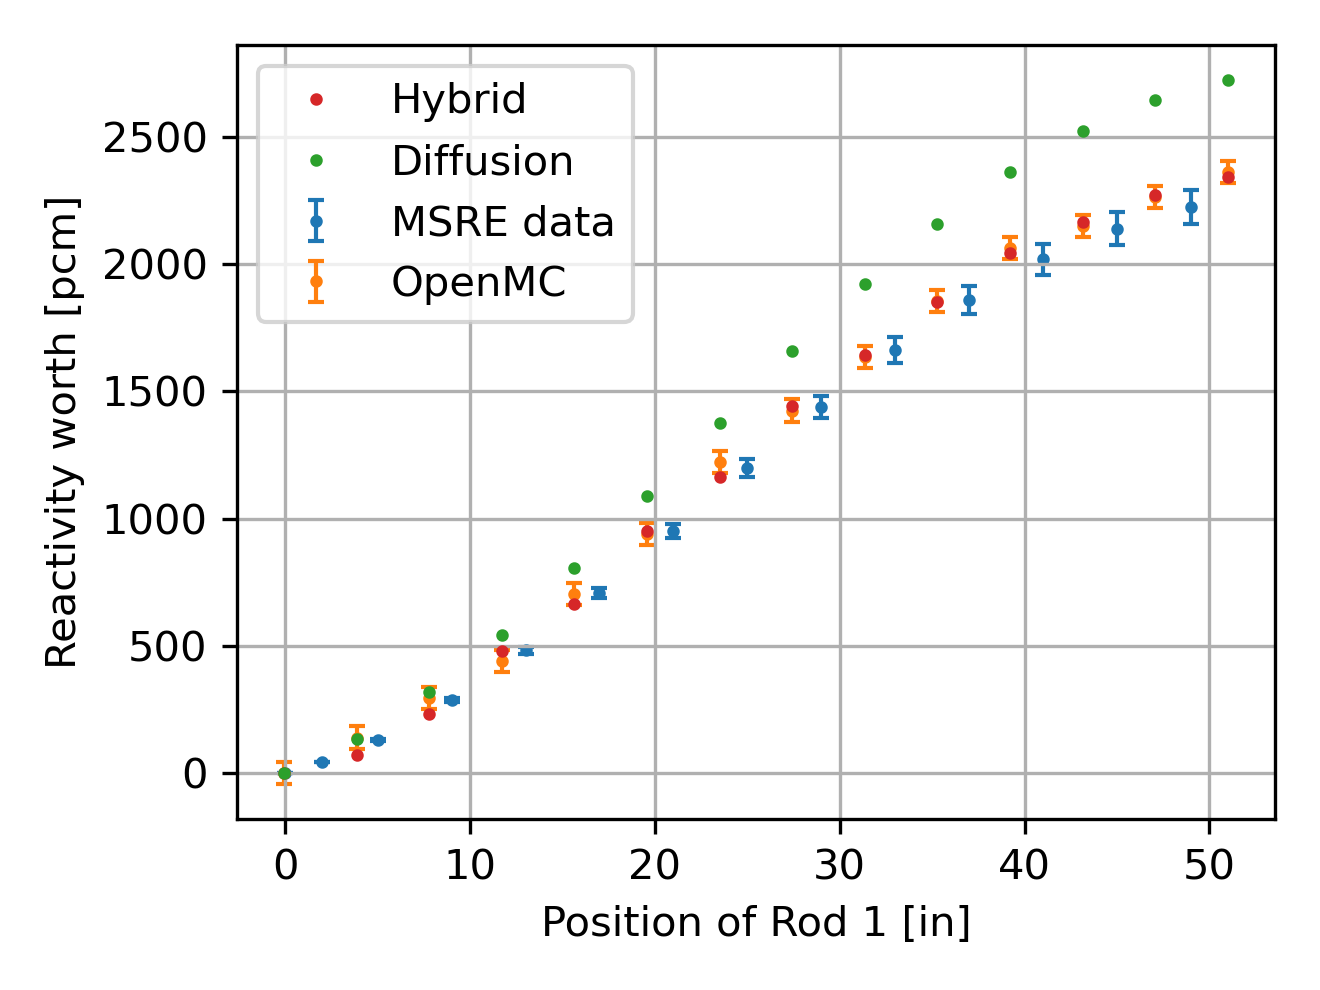
\includegraphics[width=0.8\columnwidth]{rod-worth-curve}
  \caption{Reactivity inserted by Rod 1 at various rod positions relative to the full insertion.}
  \label{fig:rod-worth}
\end{figure}

\begin{table}[t]
  \centering
  \caption{Total rod worth of Rod 1 when fully inserted.}
  \begin{tabular}{l S[table-format=4(2)] S}
    \toprule
     & {$\rho_\text{worth}$ [pcm]} & {Percentage discrepancy [\%]}\\
     \cmidrule(rl){2-2} \cmidrule(l){3-3}
    \gls{MSRE} experimental data & 2250(67) & {-}\\
    OpenMC (This work) & 2364(44) & 5.1 \\
    Hybrid (This work) & 2345 & 4.2 \\
    Diffusion (This work) & 2725 & 21.1 \\
    \bottomrule
  \end{tabular}
  \label{table:rod-worth}
\end{table}

The most likely factor for OpenMC and the hybrid method overpredicting the control rod worth is the
modeling of control rods as solid annular cylinders as opposed to 36 separate control elements
strung along a flexible stainless steel cable. Figure \ref{fig:rod-bead} depicts a poison element
and its physical dimensions. Other than the Gd$_2$O$_3$-Al$_2$O$_3$ poison material, each control
element has a top and bottom closure made of INOR-8 alloy. According to the physical dimensions,
the closures make up 15.1\% of the total element height. The 3-D numerical \gls{MSRE} model in this
work omits the outer and inner INOR-8 tubes and the flexible stainless cable, and replaces the top
and bottom closure with poison material. Fully resolving the closures in Moltres would require
excessively fine axial mesh resolution and advanced adaptive meshing features not currently
available. A straightforward corrective measure for future \gls{MSRE} simulations would be to
retain the solid annular cylinder structure and adjust the rod dimensions or the rod material
composition to match the expected worth from \gls{MSRE} data or OpenMC simulations with the beaded
geometry.

\begin{figure}[t]
  \begin{subfigure}[b]{0.33\columnwidth}
    \centering
    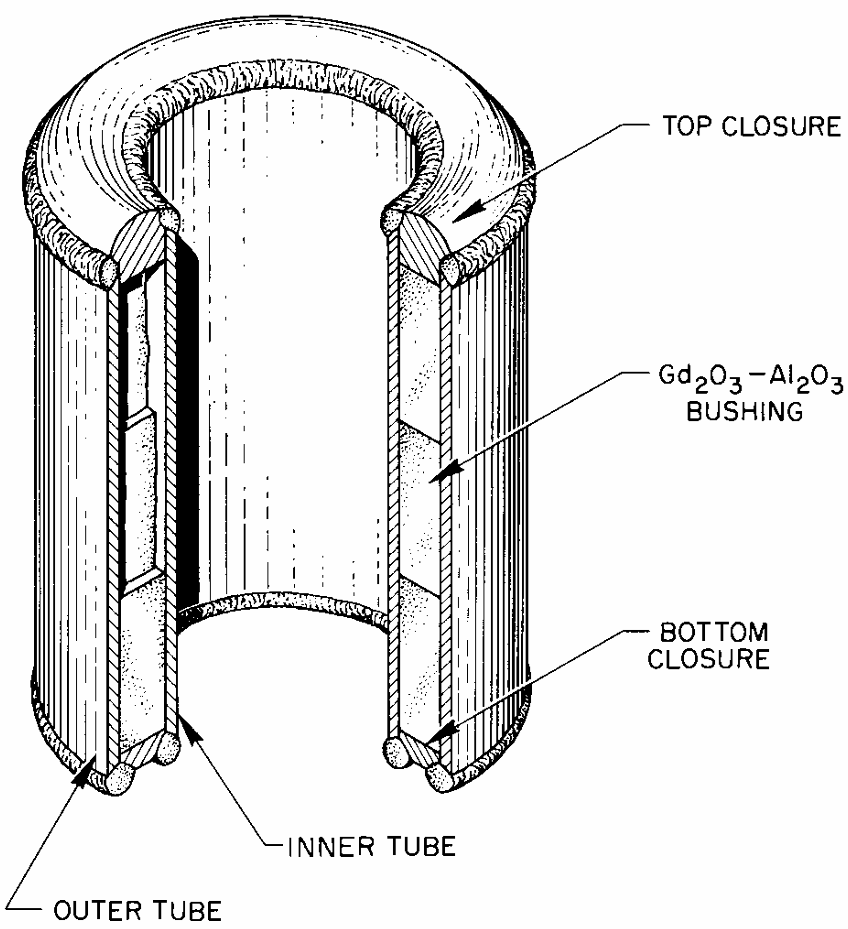
\includegraphics[width=\columnwidth]{rod-bead-2}
  \end{subfigure}
  \begin{subfigure}[b]{0.65\columnwidth}
    \centering
    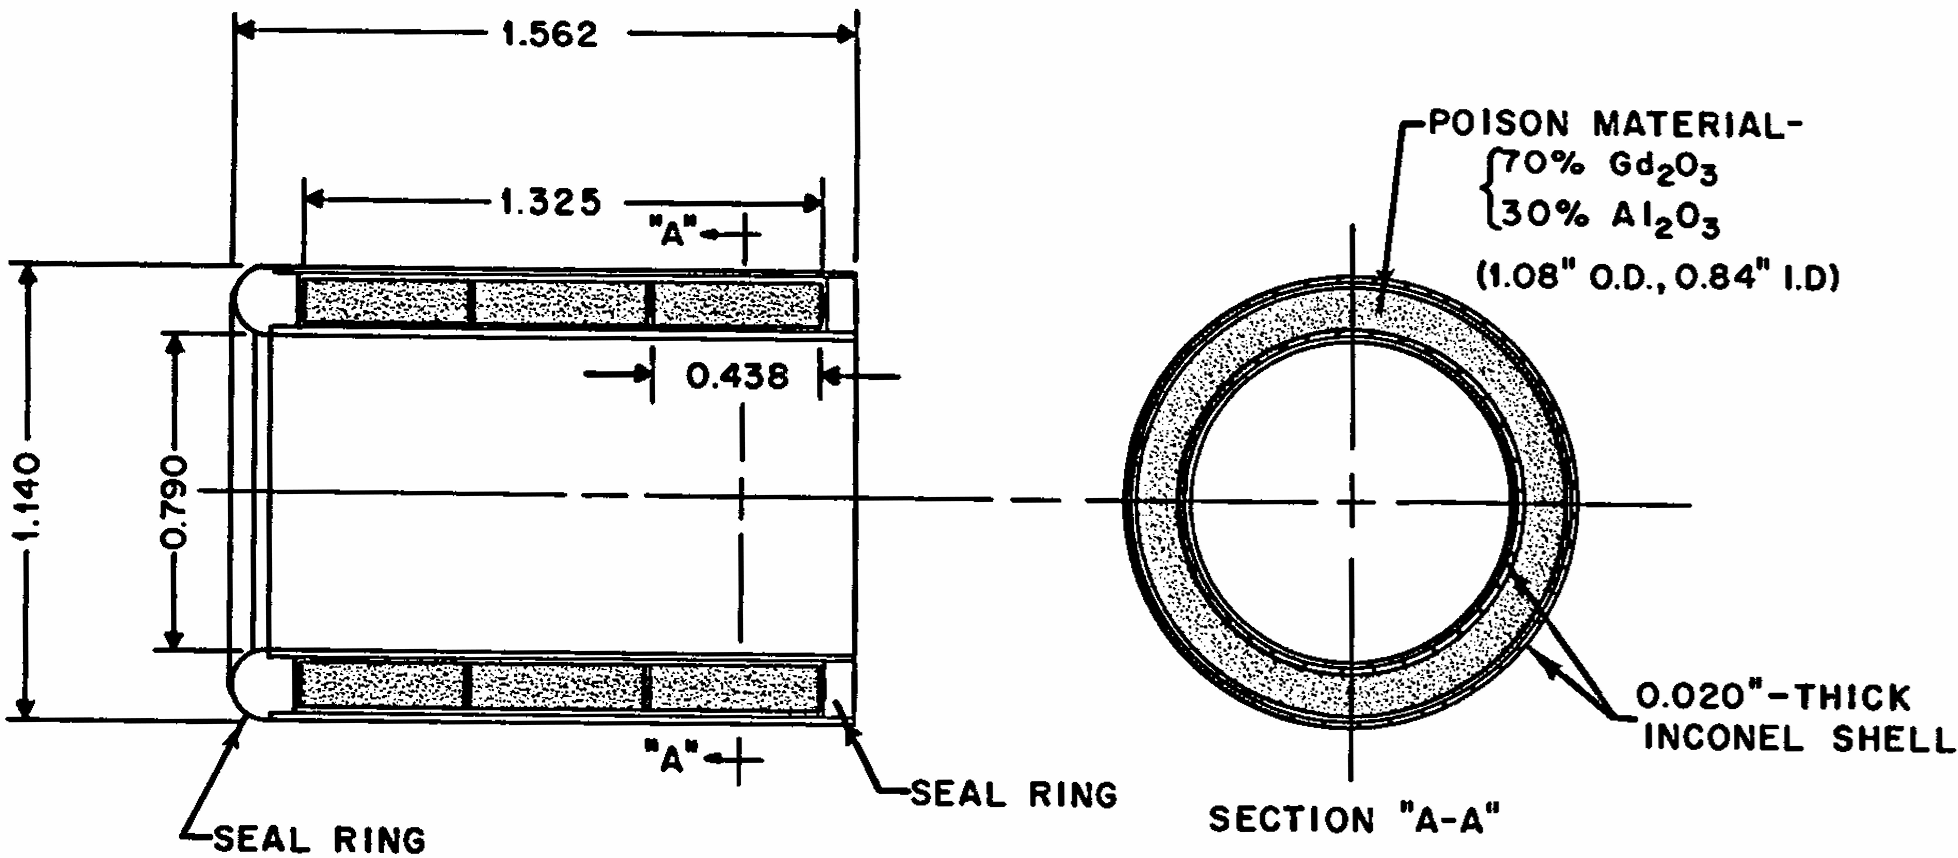
\includegraphics[width=\columnwidth]{rod-bead}
  \end{subfigure}
  \caption{Cutaway view and dimensions of a control rod poison element.}
  \label{fig:rod-bead}
\end{figure}

Overall, the results show that the hybrid $S_N$-diffusion method accurately reproduces the control
rod worth at various levels of insertion. As observed in the 1-D and 2-D models, the 3-D model
$k_\text{eff}$ values exhibit some discrepancies relative to OpenMC, but the discrepancies do not
affect rod worth estimates because they are systematic errors. This \gls{MSRE} hybrid model may be
improved in future work by characterizing and applying neutron albedo at the vacuum boundaries.

\subsubsection{Temperature Reactivity Coefficient}

This work compares isothermal temperature reactivity coefficients calculated from $k_\text{eff}$
values measured at 872 K and 972 K with 67.86 $^{235}$U loading. This approach is identical to that
of the \gls{MSRE} experimental measurements \cite{prince_zero-power_1968} and the \gls{MSRE}
numerical benchmark calculations \cite{fratoni_molten_2020}. The temperature reactivity coefficient
is calculated by dividing the difference in reactivities by the temperature change (100 K). All
simulations included the effects of thermal expansion on the material density but left all reactor
physical dimensions unchanged.

Table \ref{table:temp-coef} compares the isothermal reactivity coefficients from the experimental
and numerical sources. The OpenMC and Moltres models in this work show closer agreement with the
\gls{MSRE} data than the Serpent 2 model from the \gls{MSRE} numerical benchmark. All numerical
results fall within one standard deviation of the \gls{MSRE} data.

\begin{table}[t]
  \small
  \centering
  \caption{Isothermal temperature reactivity coefficients with 67.86 kg $^{235}$U loading from
  \gls{MSRE} data, the \gls{MSRE} numerical benchmark \cite{fratoni_molten_2020}, and the OpenMC
  and Moltres models in this work.}
  \begin{tabular}{l S[separate-uncertainty=true,table-format=2.2(2)] S}
    \toprule
     & {Temperature coefficient [pcm K$^{-1}$]} & {Percentage discrepancy [\%]}\\
     \cmidrule(rl){2-2} \cmidrule(l){3-3}
    \gls{MSRE} experimental data & 13.41(150) & {-}\\
    Serpent 2 (Numerical benchmark) & 12.51(23) & -6.7 \\
    OpenMC (This work) & 13.85(43) & 3.3 \\
    Hybrid (This work) & 13.98 & 4.3 \\
    Diffusion (This work) & 14.01 & 4.5 \\
    \bottomrule
  \end{tabular}
  \label{table:temp-coef}
\end{table}

\subsubsection{Computational Performance}

Beyond demonstrating the hybrid $S_N$-diffusion method, its computational performance is of
interest as a candidate for 3-D, time-dependent reactor simulations. All simulations ran on the
Polaris supercomputer system at \gls{ANL}. Each compute node consists of a 2.8-GHz AMD EPYC Milan
7543P 32-core CPU, four NVIDIA A100 GPUs, and 512 GB of RAM. The GPUs were not utilized in this
work. Moltres uses the \gls{MPI} communication protocol for parallelizing simulations. For this
work, simulations ran with 1-to-1 ratio of \gls{MPI} ranks and processor cores (i.e., 32 \gls{MPI}
ranks for each compute node).

Every 3-D hybrid method $k$-eigenvalue
simulation of the \gls{MSRE} consisted of 747,688,760 \glspl{DOF} and 1,690,777,728 \glspl{DOF} for
the neutron diffusion and $S_N$ components, respectively. Each \gls{DOF} corresponds to a scalar
or angular group flux variable value defined at a mesh node. Each simulation ran with the distributed
mesh feature, which partitions and distributes the mesh across however many \gls{MPI} ranks used
in the simulation. All variable and mesh-linked data are also distributed with the mesh. This
greatly reduces memory requirements compared to storing the full mesh for each \gls{MPI} rank.

Each 3-D \gls{MSRE} simulation required at least forty nodes for sufficient memory to run. This
sets a strict minimum requirement for the 3-D hybrid simulations. On forty nodes, the simulations
required approximately 2.2 h to complete for a total of 88 node-hours or 2816 core-hours. The
distributed mesh capability comes with the cost of increased data transfer times between the $S_N$
and diffusion solvers due to increased inter-core data transfers. Transfers accounted for
approximately 0.675 h or 30 \% of the total simulation time. Future research into optimizing mesh
distribution and transfer-related data caching may help to minimize data transfers and speed-up
hybrid method simulations. The solution time for the initial neutron diffusion calculation with zero
drift correction also takes up approximately 30 \% of the total simulation time. After subtracting
the minor computational cost of evaluating the drift term even if it is zero, the hybrid method
requires about four times the solution time of the standard neutron diffusion method.

For the hybrid method to be viable for large time-dependent simulations, it must scale reasonably
well on computing clusters. For this work, I investigated strong scaling, which measures how the
solution time decreases when more cores are used while keeping the problem size fixed. This strong
scaling study used 3-D quarter-core models run on 10, 20, 30, and 40 compute nodes.
Figure * shows the results of this scaling study.
The hybrid method implementation scales well as shown by the nearly linear scaling between the
solution time and the number of processors. Therefore, the hybrid method appears promising for the
modeling of larger reactor analyses with little scaling performance penalty.

% Strong scaling tests & discussion
% Difficulties with 3-D modeling
% SN void treatment constants, Transfer times

\section{Summary}

This chapter covers work demonstrating the hybrid $S_N$-diffusion method implemented in Moltres
through 1-D, 2-D, and 3-D neutronics simulations of \gls{MSRE} models. The hybrid method combines
the $S_N$
and diffusion methods by applying transport corrections generated using the high-fidelity $S_N$
method near control rods while treating the rest of the problem with the lower-fidelity diffusion
method for tractable 3-D time-dependent reactor analyses. This is achieved by identifying and
setting up a subregion containing the control rod and its vicinity for $S_N$ transport
calculations. The $S_N$ and diffusion solvers are coupled through boundary sources at the subregion
boundaries. The hybrid method applies an adaptive algorithm for discarding inaccurate transport
correction values near the subregion boundaries and preserving the smoothness of the neutron flux
gradient. In this chapter, the 1-D simulations provided verification of the hybrid method for
estimating control rod worth. The simulations also compared two different implementations of the
hybrid method which differed by the use of drift or diffusion correction schemes.
The 2-D and 3-D simulations extended the hybrid method to multi-dimensional problems. Additionally,
the 3-D simulations validated the numerical \gls{MSRE} model against \gls{MSRE} experimental data
and provided useful insight on the computational performance of the hybrid method for
large reactor analyses.

Six 1-D test cases based on the \gls{MSRE} with increasing geometric complexity were run using the
standard $S_N$ method, the hybrid method, and standard neutron diffusion method and verified against
reference OpenMC Monte Carlo neutron transport simulations under continuous neutron energy (OpenMC-CE) and
multigroup (OpenMC-MG) modes. The $S_N$ implementation with nonlinear diffusion acceleration
showed good agreement with OpenMC-MG which indicated that discrepancies between those codes and
OpenMC-CE largely arose from the eight neutron energy group structure for multigroup simulations.
Both hybrid method implementations, with drift or diffusion correction schemes, showed similar
performance in the 1-D cases. While the $k_\text{eff}$ estimates from the hybrid method deviated
from the $S_N$ method and OpenMC-MG by 100 to 400 pcm, the hybrid method accurately reproduces
control rod worths. Rod worth estimates from OpenMC-MG, $S_N$, and hybrid methods differed from
OpenMC-CE by 2 to 3 \%. The hybrid method improves on the neutron diffusion method whose rod worth
error estimate is 8 \%. The hybrid method also produced better agreement in neutron flux
distributions with the neutron transport methods compared to the neutron diffusion method.

Analysis on the drift and diffusion correction schemes showed that the diffusion correction
parameter led to numerous discontinuities tending to infinity values near points in the problem
domain where flux peaks and troughs occur. These discontinuities and negative diffusion coefficient
values are unphysical and would lead to numerical stability issues. Therefore, the hybrid method
implementation with drift correction scheme was chosen for the remaining 1-D analyses and the
2-D and 3-D analyses.

Analysis on the impact of $S_N$ correction subregion size found that it has little impact on the
control rod worth estimates as long as the subregion size is kept consistent (i.e., same size) when
performing control rod worth measurements. Rod worths varied by less than 0.35 \% across the
different subregion sizes investigated. A separate analysis showed that the $k_\text{eff}$
estimates from the hybrid method exhibit superlinear convergence rate when tightening the $S_N$
convergence tolerance value. The convergence tolerance value also impacts the number of outer
iterations between $S_N$ and diffusion solvers. After just two outer iterations, the error in
$k_\text{eff}$ fell to below 10$^{-7}$.

The hybrid method continued to show improved control rod estimates over the neutron diffusion
method in 2-D quarter-core and full-core \gls{MSRE} simulations with up to three rods inserted in the
full-core model. The hybrid method reported rod worth error magnitudes of less than 40 pcm relative
to OpenMC-CE, which are significant improvements over the neutron diffusion method error estimates
ranging from 569 pcm to 1484 pcm. The hybrid method also showed significant improvements in the
absolute mean and maximum errors in fuel channel power distributions relative to the reference
OpenMC-CE distribution.

For 3-D simulations, the \gls{MSRE} experimental data and the \gls{MSRE} numerical benchmark
report \cite{fratoni_molten_2020} both served as references for model validation. The numerical
benchmark is included in the International Reactor Physics Experiment Evaluation Project (IRPhEP)
handbook. The
$k_\text{eff}$ estimates of the \gls{MSRE} at initial criticality from OpenMC, the hybrid method,
and the neutron diffusion method in this work showed good agreement with the \gls{MSRE} numerical
benchmark. All numerical $k_\text{eff}$ estimates, including that from the benchmark report
\cite{fratoni_molten_2020}, exceeded the \gls{MSRE} experimental value by 1-2 \% due to possible
biases and uncertainties in the neutronic properties of graphite. Temperature reactivity
coefficient values from OpenMC, the hybrid method, and the neutron diffusion method also show good
agreement with the \gls{MSRE} data within experimental uncertainty with percentage discrepancies of
about 3 \%, but differ from the numerical benchmark which has a percentage discrepancy of -6.7 \%.

Control rod worth calculations were also performed for Rod 1 of the \gls{MSRE} under various levels
of insertion from its fully inserted to its fully withdrawn state. OpenMC and the hybrid method
showed excellent agreement at every stage within one standard deviation. Due to geometric
approximations of the control rods in the numerical models, they overestimated the total
rod worth relative to the \gls{MSRE} experimental data by approximately 4-5 \%. The hybrid method
compares favorably against the neutron diffusion method which overestimated the total worth by
21.1 \%.

The 3-D simulations performed well under the strong scaling test which studies how the solution
time scales with the number of processors used to run the simulation. The 3-D simulations showed
close to linear scaling within the scope of the strong scaling test. Therefore, the hybrid method
exhibits good computational scaling performance which is essential for large 3-D reactor analyses.
Excessively large memory requirements were mitigated through the distributed mesh capability in
Moltres. Some performance optimizations may be possible to reduce data transfer times
between the $S_N$ and diffusion solvers which currently take up about 30 \% of the total solution
time as a result of the inter-processor communications.

Overall, the hybrid $S_N$-diffusion method provides a significant improvement over the neutron
diffusion method at only four times the computational expense. Control rod estimates
show good agreement with reference Monte Carlo solutions and \gls{MSRE} experimental data.
Further investigations into characterizing and minimizing neutron leakage rates at vacuum
boundaries may help with reducing $k_\text{eff}$ discrepancies with reference Monte Carlo
solutions.
